% =====================================================================
%  Forty Points: one qutrit, the exceptional algebras, and a light cone
%  A synthesis of the W(3,3) programme for every reader.
%  Compile with tectonic (XeTeX):  tectonic -X compile main.tex
% =====================================================================
\documentclass[11pt,twoside]{article}

% ---------------------------------------------------------------- fonts
\usepackage{amsmath,amsthm,mathtools}% must precede unicode-math
\usepackage{fontspec}
\usepackage{unicode-math}
\setmainfont{texgyrepagella}[Extension=.otf,UprightFont=*-regular,BoldFont=*-bold,
  ItalicFont=*-italic,BoldItalicFont=*-bolditalic]
\setsansfont{texgyreheros}[Extension=.otf,UprightFont=*-regular,BoldFont=*-bold,
  ItalicFont=*-italic,BoldItalicFont=*-bolditalic,Scale=0.92]
\setmonofont{texgyrecursor}[Extension=.otf,UprightFont=*-regular,BoldFont=*-bold,
  ItalicFont=*-italic,BoldItalicFont=*-bolditalic,Scale=0.95]
\setmathfont{texgyrepagella-math.otf}

% ---------------------------------------------------------------- layout
\usepackage[a4paper,inner=30mm,outer=26mm,top=28mm,bottom=30mm,headsep=10mm]{geometry}
\usepackage{microtype}
\raggedbottom
\usepackage{booktabs,array,tabularx,longtable,multirow}
\usepackage{enumitem}
\usepackage{xcolor}
\usepackage{graphicx}
\usepackage{tikz}
\usetikzlibrary{arrows.meta,positioning,calc,decorations.pathreplacing,shapes.geometric,backgrounds,fit}
\usepackage[most]{tcolorbox}
\usepackage{titlesec}
\usepackage{fancyhdr}
\usepackage{etoolbox}
\usepackage{xurl}
\usepackage[font=small,labelfont={bf,sf,color=ink},labelsep=period,margin=4mm]{caption}
\newcommand{\computed}{\textcolor{teal!80!black}{\boldmath$\surd$}}
\usepackage[hidelinks,bookmarksnumbered]{hyperref}
\setlength{\parskip}{0.45em}
\setlength{\parindent}{0pt}
\linespread{1.06}
\setlist{itemsep=2pt,topsep=4pt}

% ---------------------------------------------------------------- palette
\definecolor{ink}{HTML}{1B2A41}
\definecolor{teal}{HTML}{0F7C80}
\definecolor{tealsoft}{HTML}{E6F4F3}
\definecolor{gold}{HTML}{B7791F}
\definecolor{goldsoft}{HTML}{FBF3E4}
\definecolor{rose}{HTML}{B4415A}
\definecolor{rosesoft}{HTML}{FBEDEF}
\definecolor{sky}{HTML}{3C6FB4}
\definecolor{skysoft}{HTML}{EAF1FA}
\definecolor{sage}{HTML}{4E8A4A}
\definecolor{sagesoft}{HTML}{EEF6EC}
\definecolor{slate}{HTML}{5B6573}
\definecolor{paper}{HTML}{FFFDF8}
% figure fills
\colorlet{orgn}{ink!85}
\colorlet{nullc}{gold!55}
\colorlet{plusc}{teal!35}
\colorlet{minusc}{rose!30}

% ---------------------------------------------------------------- headings
\titleformat{\section}{\sffamily\Large\bfseries\color{ink}}{\color{teal}\thesection}{0.8em}{}
  [{\color{teal}\titlerule[0.8pt]}]
\titleformat{\subsection}{\sffamily\large\bfseries\color{ink}}{\color{teal}\thesubsection}{0.7em}{}
\titleformat{\subsubsection}{\sffamily\normalsize\bfseries\color{slate}}{\thesubsubsection}{0.6em}{}
\titlespacing*{\section}{0pt}{2.2em}{1.1em}
\titlespacing*{\subsection}{0pt}{1.6em}{0.6em}

\pagestyle{fancy}
\fancyhf{}
\fancyhead[LE]{\sffamily\small\color{slate}\thepage\quad\textbar\quad Forty Points}
\fancyhead[RO]{\sffamily\small\color{slate}\nouppercase{\leftmark}\quad\textbar\quad\thepage}
\renewcommand{\headrulewidth}{0pt}
\renewcommand{\sectionmark}[1]{\markboth{#1}{}}

% ---------------------------------------------------------------- tiers
\newtcbox{\tierbox}[1][teal]{on line,colback=#1,colframe=#1,coltext=white,
  boxrule=0pt,arc=2pt,left=2.5pt,right=2.5pt,top=0.5pt,bottom=0.5pt,fontupper=\sffamily\scriptsize\bfseries}
\newcommand{\tierT}{\tierbox[teal]{THEOREM}}
\newcommand{\tierC}{\tierbox[sky]{COMPUTATION}}
\newcommand{\tierB}{\tierbox[gold]{BRIDGE}}
\newcommand{\tierX}{\tierbox[rose]{REFUTED}}
\newcommand{\tierO}{\tierbox[slate]{OPEN}}

% ---------------------------------------------------------------- boxes
\newtcolorbox{plainwords}[1][In plain words]{enhanced,breakable,
  colback=goldsoft,colframe=gold!70,boxrule=0pt,leftrule=3pt,arc=0pt,
  left=10pt,right=10pt,top=6pt,bottom=6pt,
  fonttitle=\sffamily\bfseries\small,coltitle=gold!80!black,
  attach title to upper={\par\smallskip},title={#1}}
\newtcolorbox{physical}[1][What it means physically]{enhanced,breakable,
  colback=tealsoft,colframe=teal,boxrule=0pt,leftrule=3pt,arc=0pt,
  left=10pt,right=10pt,top=6pt,bottom=6pt,
  fonttitle=\sffamily\bfseries\small,coltitle=teal!80!black,
  attach title to upper={\par\smallskip},title={#1}}
\newtcolorbox{boundary}[1][Where this stops]{enhanced,breakable,
  colback=rosesoft,colframe=rose,boxrule=0pt,leftrule=3pt,arc=0pt,
  left=10pt,right=10pt,top=6pt,bottom=6pt,
  fonttitle=\sffamily\bfseries\small,coltitle=rose!85!black,
  attach title to upper={\par\smallskip},title={#1}}
\newtcolorbox{result}[2][]{enhanced,breakable,
  colback=white,colframe=ink!55,boxrule=0.6pt,arc=2pt,
  left=10pt,right=10pt,top=7pt,bottom=7pt,
  colbacktitle=skysoft,coltitle=ink,fonttitle=\sffamily\bfseries\small,
  title={#2},#1}
\newtcolorbox{keyidea}{enhanced,colback=ink,colframe=ink,coltext=white,arc=3pt,
  boxrule=0pt,left=12pt,right=12pt,top=9pt,bottom=9pt,fontupper=\large\itshape}

% ---------------------------------------------------------------- theorems
\theoremstyle{plain}
\newtheorem{theorem}{Theorem}[section]
\newtheorem{proposition}[theorem]{Proposition}
\newtheorem{lemma}[theorem]{Lemma}
\newtheorem{corollary}[theorem]{Corollary}
\theoremstyle{definition}
\newtheorem{definition}[theorem]{Definition}
\newtheorem{example}[theorem]{Example}
\theoremstyle{remark}
\newtheorem*{remark}{Remark}

% ---------------------------------------------------------------- notation
\newcommand{\F}{\mathbb{F}}
\newcommand{\C}{\mathbb{C}}
\newcommand{\R}{\mathbb{R}}
\newcommand{\Z}{\mathbb{Z}}
\newcommand{\Q}{\mathbb{Q}}
\newcommand{\W}{W(3,3)}
\newcommand{\e}{\mathfrak{e}}
\newcommand{\g}{\mathfrak{g}}
\newcommand{\sll}{\mathfrak{sl}}
\newcommand{\so}{\mathfrak{so}}
\newcommand{\Sp}{\mathrm{Sp}}
\newcommand{\PSp}{\mathrm{PSp}}
\newcommand{\PGSp}{\mathrm{PGSp}}
\newcommand{\SRG}{\mathrm{SRG}}
\newcommand{\End}{\mathrm{End}}
\newcommand{\ad}{\mathrm{ad}}
\newcommand{\tr}{\operatorname{tr}}
\newcommand{\ket}[1]{\lvert #1\rangle}
\newcommand{\bra}[1]{\langle #1\rvert}
\newcommand{\cert}[1]{\begingroup\ttfamily\small\color{ink!80}%
  \def\_{\char`\_\penalty0\hskip0pt plus 1pt\relax}#1\endgroup}
\newcommand{\hgt}{\operatorname{ht}}

\hypersetup{pdftitle={Forty Points: One Qutrit, the Exceptional Algebras, and a Light Cone},
  pdfauthor={The W(3,3) Theory Programme}}

\begin{document}
\pagecolor{paper}

% ================================================================= title
\begin{titlepage}
\thispagestyle{empty}
\centering
\vspace*{8mm}
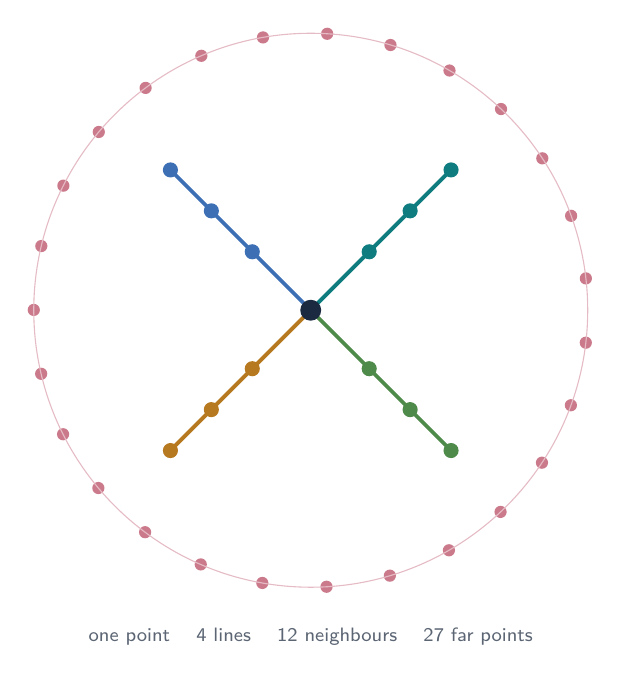
\begin{tikzpicture}[scale=1.05]
  % the 1 + 12 + 27 structure seen from one point of W(3,3)
  \foreach \k in {0,...,26}{
    \fill[rose!70] ({360*\k/27+6.6}:3.35) circle (2.1pt);}
  \draw[rose!35,line width=0.4pt] (0,0) circle (3.35);
  \foreach \a/\c in {45/teal,135/sky,225/gold,315/sage}{
    \draw[\c,line width=1.4pt] (0,0) -- (\a:2.45);
    \foreach \r in {1.0,1.7,2.4}{\fill[\c] (\a:\r) circle (2.6pt);}}
  \fill[ink] (0,0) circle (3.6pt);
  \node[font=\sffamily\scriptsize,text=slate] at (0,-3.95) {one point \quad 4 lines \quad 12 neighbours \quad 27 far points};
\end{tikzpicture}

\vspace{12mm}
{\sffamily\fontsize{30}{36}\selectfont\bfseries\color{ink} Forty Points\par}
\vspace{4mm}
{\Large\itshape\color{teal} One qutrit, the exceptional algebras, and a light cone\par}
\vspace{9mm}
{\large An exact and honest account of the $W(3,3)$ programme,\\
written so that anyone can follow it\par}
\vspace{12mm}
{\sffamily\color{slate} The W(3,3) Theory Programme\\[2pt]
\small repository \texttt{wilcompute/W33-Theory}\quad$\cdot$\quad 26 September 2026\par}
\vfill
\begin{minipage}{0.86\textwidth}\small\color{slate}
Every mathematical statement in this paper carries a status badge and, where it is
a computation, the path of the committed script and certificate that proves it.
Interpretations are labelled as interpretations. Things that were believed and later
shown false are kept on the page, with the measurement that overturned them.
\end{minipage}
\vspace{6mm}
\end{titlepage}

% ================================================================= abstract
\thispagestyle{empty}
\section*{Abstract}
\addcontentsline{toc}{section}{Abstract}

\textbf{For everyone.} Take the smallest quantum system that has three settings
instead of two --- a \emph{qutrit} --- and let it act on itself. The ways it can be
transformed, and the ways those transformations do or do not interfere with one
another, form a finite geometric object with exactly forty points. This paper follows
that single object as far as exact mathematics can take it. It turns out to contain
a tiny version of space-time with a light cone; four interlocking ``clocks''; the
largest exceptional symmetry in mathematics, $E_8$; the octonionic algebra of
$3\times3$ matrices that physicists have long suspected sits behind particle physics;
and, inside that algebra, a genuine ten-dimensional Lorentz group whose spinors are
the matter particles of one generation. We also say, just as clearly, what the
object does \emph{not} do: it does not by itself produce the masses, the forces, or
the dynamics of our universe, and it provably cannot decide whether nature is
left-handed or right-handed. Finally we settle, by an exhaustive exact computation, the
most important open question about the string-theory models built on it: in their
supersymmetric vacua the proton is not protected, because a field with the quantum numbers
of a right-handed sneutrino is forced to condense --- and that field carries exactly the charge
that switches the forbidden couplings back on. We follow every escape route we could find to
its end: other discrete symmetries, parities built from rotations of the hidden dimensions,
and very heavy superpartners. Each fails --- one only after we found that the selection rule it
relied on is incomplete --- and the last would need a top quark lighter than the one we measure.

\medskip
\textbf{For specialists.} The symplectic generalized quadrangle $\W$ is the projective
commutation geometry of the two-sided Weyl action on one qutrit's Hilbert--Schmidt
space; its Bell line is the unitary-channel diagonal. Fixing that line, the
$27$ transverse Lagrangians form $\mathrm{Sym}_2(\F_3)$ with the finite Minkowski form
$t^2-x^2-y^2$, whose null relation is context intersection; the four null directions
are $\mathbb{P}^1(\F_3)$, the tetracode is their evaluation code, and the same four
labels index the Hesse striations and an $A_2^4\subset E_8$. On the committed
executable $E_8$ Chevalley basis, a Hesse tick line induces the contact grading
$1+56+134+56+1$; its $56$ is exactly the Freudenthal triple system of the split Albert
algebra whose norm is the repository's signed $45$-triad $E_6$ cubic,
$Q=(\alpha\beta+T)^2-4\beta N(X)-4\alpha N(Y)+4T(X^\#,Y^\#)$, and the $57$-dimensional
Heisenberg extension carries the quasiconformal cone $N=Q/4-\tau^2$ with the
G\"unaydin--Koepsell--Nicolai inversion law. The Killing form obeys
$K(e_\alpha,e_{-\alpha})=-60(-1)^{\operatorname{ht}\alpha}$; the three tick lines give
commuting $E_{8(-24)}$ involutions with $E_8=80+56+56+56$, restricting to $E_{7(-25)}$,
whose Hermitian Jordan triple yields a Euclidean Albert algebra with Peirce split
$1+16+10$, a Lorentzian $(1,9)$ Peirce slice, $\mathrm{Der}=F_{4(-52)}$,
$\mathrm{str}_0=E_{6(-26)}$, and an $\mathfrak{so}(1,9)$ acting on a Majorana--Weyl $16$.
The repository's matter-parity charge is $6L_c-2$, and matter parity is the $2\pi$
rotation of $\mathrm{Spin}(9)$. The committed split real form, by contrast, is the
height twist $\exp(i\pi\rho^\vee)$ and gives a $(5,5)$ slice: signature is a real-form
datum, invisible over $\F_3$. For the $215$ heterotic $\Z_6$ Standard Models of the $\W$
twist we recover and freeze the exact spectra and prove, over the full rational $B-L$
freedom and over all $1024$ $\Z_2$ characters odd on quarks and leptons, that no
FI-cancelling $D$-flat singlet vacuum preserves matter parity: the never-even singlets have
$B-L=\pm1$ and every $D$-flat vacuum condenses one. The obstruction is one $E_6$-shaped $U(1)$,
$4Q_\psi-\tfrac45Q_\chi$; it extends to every element of the gauge torus times the space group
(Smith normal forms), the forced field obeys $Q(n)=-Q(u^cd^cd^c)=-Q(q\ell d^c)=-Q(\ell\ell e^c)$ and
regenerates all three couplings at quartic order, and baryon triality is excluded by
$Q(u^c)+Q(e^c)=2Q(q)$. Plane-rotation $R$-symmetries appear to reopen parity in one model, but only
through an $R$-rule that is incomplete on non-prime planes; with the rules derived from the worldsheet
instantons (Bizet et al.) the $\Z_6$-II class closes ($0/128$), as do the $\Z_2\times\Z_6$ and $\Z_3\times\Z_6$
families of the same twist; and
two-loop running of the Higgs quartic caps any superpartner scale that could tame the regenerated
couplings unless $m_t\le171$\,GeV.

\vspace{6mm}
\begin{keyidea}
The forty points are forty views of one thing. Looked at through the right lens, the
same finite object is a quantum measurement geometry, a finite space-time, a clock, a
lattice, an exceptional Lie algebra, and a Lorentzian light cone --- and each
identification in this paper is an exact computation, not an analogy.
\end{keyidea}

\clearpage
\tableofcontents
\clearpage

\section*{How to read this paper}
\addcontentsline{toc}{section}{How to read this paper}
\markboth{How to read this paper}{}

This paper is written for two readers at once. One has never studied algebra beyond
school and wants to understand what has actually been found. The other wants every
statement to be precise enough to check. We have tried not to cheat either of them.
The mathematics is stated in full; next to it, in gold-edged boxes, the same idea is
explained in ordinary words, and in teal-edged boxes we say what the idea means
physically. Rose-edged boxes mark the edge of what is known.

\subsection*{The five badges}

Every claim of substance carries one of five labels. They are the most important
typographical device in the paper, because the whole value of a speculative subject
lies in being able to tell the proved from the hoped-for.

\begin{center}
\renewcommand{\arraystretch}{1.35}
\begin{tabularx}{0.95\textwidth}{@{}lX@{}}
\toprule
\tierT & A mathematical theorem: proved by an argument in the text, or a standard result
         with a reference. \\
\tierC & An exact finite computation, carried out by a committed script whose output
         certificate is named. ``Exact'' means integer or rational arithmetic, or an
         exhaustive enumeration --- never a numerical approximation, unless we say so. \\
\tierB & A bridge: a mathematically true statement \emph{plus} an interpretation of it
         (for example, calling a mathematical light cone a light cone of time). The
         mathematics is certain; the interpretation is a proposal. \\
\tierO & An open question, stated as sharply as we can. \\
\tierX & Something that was once believed, written down, and then shown false. We keep
         these, with the reason. \\
\bottomrule
\end{tabularx}
\end{center}

\subsection*{A map of the journey}

The paper follows one chain of exact identifications. Figure~\ref{fig:journey} is the
whole argument in one picture; each box is a section.

\begin{figure}[htbp]
\centering
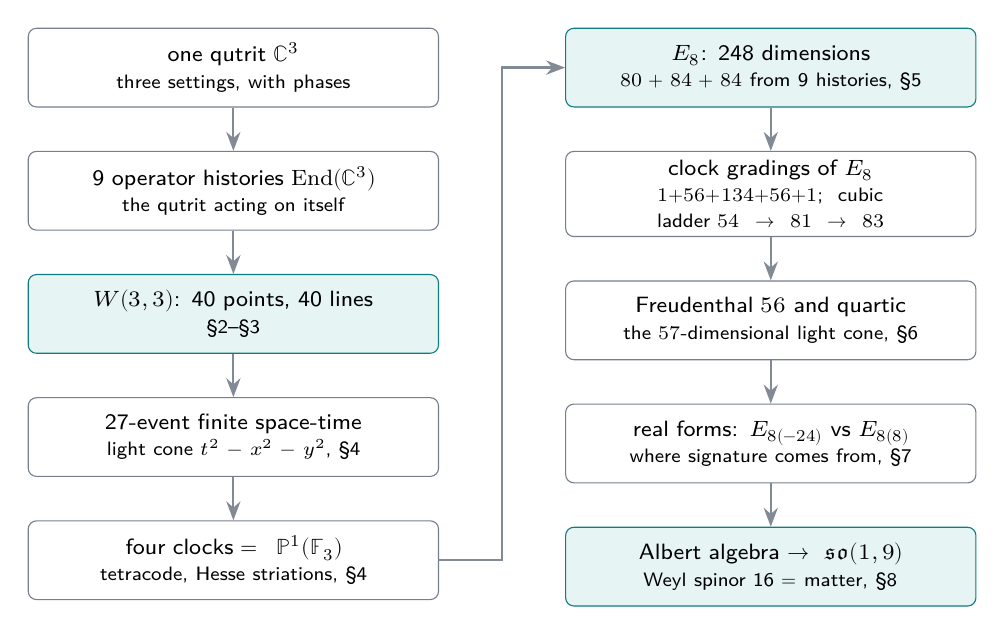
\begin{tikzpicture}[
  node distance=5.5mm and 16mm,
  st/.style={draw=ink!60,rounded corners=3pt,fill=white,align=center,
    font=\sffamily\footnotesize,text width=50mm,minimum height=10mm,inner sep=3pt},
  hl/.style={st,fill=tealsoft,draw=teal},
  ar/.style={-{Stealth[length=2.4mm]},thick,ink!55}]
  \node[st] (q) {one qutrit $\C^3$\\\scriptsize three settings, with phases};
  \node[st,below=of q] (h) {9 operator histories $\End(\C^3)$\\\scriptsize the qutrit acting on itself};
  \node[hl,below=of h] (w) {$\W$: 40 points, 40 lines\\\scriptsize \S2--\S3};
  \node[st,below=of w] (m) {27-event finite space-time\\\scriptsize light cone $t^2-x^2-y^2$, \S4};
  \node[st,below=of m] (c) {four clocks $=\mathbb{P}^1(\F_3)$\\\scriptsize tetracode, Hesse striations, \S4};
  \node[hl,right=of q] (e8) {$E_8$: 248 dimensions\\\scriptsize $80+84+84$ from 9 histories, \S5};
  \node[st,below=of e8] (gr) {clock gradings of $E_8$\\\scriptsize $1{+}56{+}134{+}56{+}1$; \ cubic ladder $54\to81\to83$};
  \node[st,below=of gr] (f) {Freudenthal $56$ and quartic\\\scriptsize the $57$-dimensional light cone, \S6};
  \node[st,below=of f] (r) {real forms: $E_{8(-24)}$ vs $E_{8(8)}$\\\scriptsize where signature comes from, \S7};
  \node[hl,below=of r] (l) {Albert algebra $\to\mathfrak{so}(1,9)$\\\scriptsize Weyl spinor 16 $=$ matter, \S8};
  \draw[ar] (q)--(h); \draw[ar] (h)--(w); \draw[ar] (w)--(m); \draw[ar] (m)--(c);
  \draw[ar] (c.east) -- ++(8mm,0) |- (e8.west);
  \draw[ar] (e8)--(gr); \draw[ar] (gr)--(f); \draw[ar] (f)--(r); \draw[ar] (r)--(l);
\end{tikzpicture}
\caption{The chain of exact identifications followed in this paper. Shaded boxes are the
three places where the story changes scale: from a qubit-sized object to a finite
geometry, from the geometry to $E_8$, and from $E_8$ to a Lorentzian algebra.}
\label{fig:journey}
\end{figure}

\subsection*{What you will need}

Nothing beyond patience. We introduce every structure before we use it, and the
glossary in Appendix~B collects the vocabulary. Readers who want only the story can
read the plain-words boxes and the key-idea panels and skip the displayed mathematics;
nothing essential will be lost. Readers who want only the mathematics can do the
reverse.

\subsection*{Where the material comes from}

Everything here is drawn from the public repository \texttt{wilcompute/W33-Theory},
a record of several thousand numbered ``passes'' by two independent research tracks,
and from its three long manuscripts --- the $\W$ paper, the photonic Holonet paper and
the Holonet machine blueprint --- some of whose pages are adapted here. Passes 10949 and
10950, which supply Sections 6--8, were carried out for this synthesis. A reader who
wants to check a statement can find its script and certificate in the ledger of
Appendix~A.

\section{Prologue: a shape made of measurements}
\label{sec:prologue}

\subsection{Why look at something finite?}

Physics describes the world with continuous quantities: positions, times, field
strengths, each a real number that can be divided forever. Yet the deepest facts we
know about nature are \emph{discrete}. An electron's spin, measured along any axis,
gives one of exactly two answers. Quarks come in exactly three colours. There are
exactly three generations of matter. The symmetry groups that organise the forces ---
$SU(3)$, $SU(2)$, $U(1)$ --- are continuous, but their representations, which decide
what particles can exist, are labelled by whole numbers.

This programme starts from the discrete end. It asks: is there a single finite object,
small enough to write down completely, whose structure already contains the patterns
physics keeps finding? The candidate studied here is a configuration of forty points
called $\W$. It is not new --- geometers have known it for a century --- but it has an
unusual habit: every time it is examined through a different lens, it turns out to be
a well-known structure from a different part of mathematics or physics. This paper is
an account of those lenses, and of exactly how far each one reaches.

\begin{plainwords}
A useful picture: $\W$ is like a crystal. A crystal is finite in its unit cell, but
the unit cell determines the whole crystal's behaviour --- how it breaks, how light
passes through it, what sounds it makes. The hope of this programme is that $\W$ is a
unit cell for something larger. The honest answer, as you will see, is that it is
a remarkable unit cell for the \emph{symmetries} of physics, and a much weaker one for
its \emph{dynamics}.
\end{plainwords}

\subsection{Bits, trits and qutrits}

Every computer you have used stores information as bits --- switches that are either
off or on. A \emph{trit} is a three-way switch: $0$, $1$, or $2$. On its own that is
not interesting; two bits can imitate a trit. A \emph{qutrit} is different. It is a
physical system with three distinguishable states, obeying quantum mechanics, which
means it can be in a blend of all three settings at once, with relative phases. In
symbols, a qutrit state is a unit vector
\[
\ket{\psi}=a_0\ket{0}+a_1\ket{1}+a_2\ket{2}\in\C^3 ,
\]
and the phases of the complex numbers $a_j$ matter.

Two operations generate everything one can do to the ``shape'' of a qutrit. The
\emph{shift} $X$ moves each setting to the next, and the \emph{clock} $Z$ stamps each
setting with a phase:
\[
X\ket{j}=\ket{j+1 \bmod 3},\qquad Z\ket{j}=\omega^{j}\ket{j},\qquad \omega=e^{2\pi i/3}.
\]
They do not commute: $ZX=\omega\,XZ$. That single twist --- a phase of one third of a
turn picked up when the order of two operations is swapped --- is the seed of
everything in this paper.

\begin{physical}
$X$ and $Z$ are the finite versions of the two most important operations in quantum
mechanics: translation in position and translation in momentum. The relation
$ZX=\omega XZ$ is the three-state version of Heisenberg's $[x,p]=i\hbar$. Physicists
call the group generated by $X$, $Z$ and the phases the \emph{Heisenberg--Weyl group};
its elements are the qutrit \emph{Pauli operators}. They label the possible
measurements one can make on a qutrit that are ``as simple as possible'' --- the
ones every other measurement is built from.
\end{physical}

\subsection{Arithmetic with three numbers}

Because $X^3=Z^3=1$, exponents only matter modulo $3$. We therefore work in the
\emph{field with three elements}, $\F_3=\{0,1,2\}$, where addition and multiplication
are done modulo $3$ --- clock arithmetic on a three-hour clock. It is a genuine
number system: every nonzero element has an inverse ($1\cdot1=1$, $2\cdot2=4=1$).
In particular $2=-1$ and $\tfrac12=2$, facts we will use repeatedly.

A qutrit Pauli operator is named by two numbers, $X^aZ^b$ with $(a,b)\in\F_3^2$.
Two qutrits need four: $(a_1,b_1,a_2,b_2)\in\F_3^4$, a space with $3^4=81$ points.

\subsection{The forty in one breath}

Here is the whole construction, which Sections~\ref{sec:object}--\ref{sec:self} unpack
slowly. Label the $81$ two-qutrit Pauli operators by vectors $x\in\F_3^4$. Remove the
identity, leaving $80$. An operator and its inverse describe the same measurement
(one is the other run backwards), and $x$ and $-x=2x$ label that pair, so the distinct
measurements number
\[
\frac{3^4-1}{3-1}=\frac{80}{2}=40 .
\]
Two of these forty measurements can be performed together exactly when their operators
commute. Recording which pairs commute gives the forty-point geometry $\W$.

\begin{keyidea}
The forty points of $W(3,3)$ are the forty independent directions along which a pair
of qutrits --- or, as Section~3 shows, one qutrit acting on itself --- can be measured.
The lines of the geometry are the complete sets of measurements that can be made at the
same time.
\end{keyidea}

\subsection{What this paper claims, and what it does not}

A ``theory of everything'' should, at a minimum, reproduce the particles and forces of
the Standard Model, the geometry of space-time and gravity, and the numbers --- masses,
couplings, mixing angles --- that we measure. It is important to say at the start that
nothing in this paper achieves that. What it does achieve is a tight web of \emph{exact}
connections between a single finite object and the structures that any such theory
seems to need:
\begin{itemize}
\item the qutrit Heisenberg group and its Clifford symmetries (Sections 2--3);
\item a finite space-time with a light cone, finite clocks, and a rigorous distinction
      between reversible time and an arrow of time (Section 4);
\item the exceptional Lie algebra $E_8$ and its subalgebras $E_7$ and $E_6$ (Section 5);
\item the Freudenthal triple system behind four-dimensional black-hole charges, and a
      $57$-dimensional light cone on which $E_8$ acts by conformal-like maps (Section 6);
\item the octonionic Albert algebra, the Lorentz algebra $\so(1,9)$ and its chiral
      spinor, which carries exactly the quantum numbers of one generation of matter
      (Sections 7--8).
\end{itemize}
Section~9 is devoted to the physics that has been attempted on top of this --- string
compactifications that realise the Standard Model on the same structure --- including
the negative results, and Section~10 to a quantum computer architecture read off the
same geometry. The Epilogue lists what remains open.

\begin{boundary}
The finite geometry supplies \emph{symmetry and structure}. It does not, by itself,
supply a Hamiltonian, an energy scale, a value of Newton's constant, or a reason for any
particular mass. Where this paper uses words like ``time'', ``light cone'' or ``matter'',
it is naming a mathematical structure that behaves like the physical one; whether nature
uses it is a separate, empirical question.
\end{boundary}

\section{The object: the symplectic quadrangle \texorpdfstring{$W(3,3)$}{W(3,3)}}
\label{sec:object}

\subsection{Definition}

Let $V=\F_3^4$ with coordinates $x=(x_1,x_2,x_3,x_4)$ and the \emph{symplectic form}
\[
\langle x,y\rangle \;=\; x_1y_3+x_2y_4-x_3y_1-x_4y_2 \pmod 3 .
\]
It is bilinear, alternating ($\langle x,x\rangle=0$) and nondegenerate (only $x=0$ pairs
to zero with everything).

\begin{definition}
The \emph{points} of $\W$ are the one-dimensional subspaces of $V$ ($40$ of them). Two
distinct points $\langle x\rangle,\langle y\rangle$ are \emph{collinear} if
$\langle x,y\rangle=0$. The \emph{lines} of $\W$ are the two-dimensional subspaces $L$
on which the form vanishes identically (\emph{totally isotropic} or \emph{Lagrangian}
planes); each contains $(9-1)/2=4$ points.
\end{definition}

\begin{result}{Proposition 2.1 \hfill \tierT}
$\W$ has $40$ points and $40$ lines. Every line has $4$ points and every point lies on
$4$ lines. For a point $p$ and a line $L$ not containing it, exactly one point of $L$ is
collinear with $p$.
\end{result}

\begin{proof}
Points: $(3^4-1)/(3-1)=40$. For a point $p=\langle x\rangle$, the set
$x^\perp=\{y:\langle x,y\rangle=0\}$ is a $3$-dimensional subspace containing $x$; the
lines through $p$ are the $2$-dimensional subspaces of $x^\perp$ that contain $x$, and
these correspond to the points of $x^\perp/\langle x\rangle\cong\F_3^2$, of which there
are $(9-1)/2=4$. Double counting point--line incidences, $40\cdot4=(\#\text{lines})\cdot4$,
so there are $40$ lines. Finally, if $p\notin L$ then $x^\perp\cap L$ is a subspace of
$L$ of dimension $1$ (it cannot be all of $L$, since then $\langle x\rangle+L$ would be a
totally isotropic $3$-space, impossible in a nondegenerate $4$-space), so exactly one
point of $L$ is collinear with $p$.
\end{proof}

The last property is the defining axiom of a \emph{generalized quadrangle}: there are no
triangles made of three lines, but from any point you can always reach any line in one
step, in exactly one way. With four points per line and four lines per point, $\W$ is
the generalized quadrangle of order $(3,3)$, usually written $\mathrm{GQ}(3,3)$ \cite{PayneThas}.

\begin{figure}[htbp]
\centering
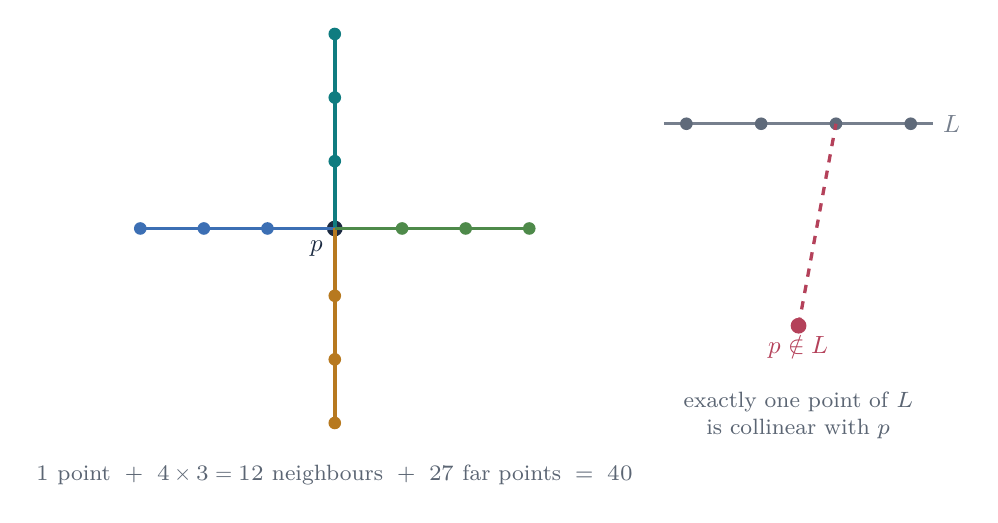
\begin{tikzpicture}[scale=0.95]
  \fill[ink] (0,0) circle (3pt) node[below left=1pt,font=\small] {$p$};
  \foreach \a/\c/\n in {90/teal/1,180/sky/2,270/gold/3,0/sage/4}{
    \draw[\c,line width=1.3pt] (0,0) -- (\a:2.6);
    \foreach \r in {0.9,1.75,2.6}{\fill[\c] (\a:\r) circle (2.4pt);} }
  \node[font=\footnotesize,align=center,text=slate] at (0,-3.3)
     {$1$ point \;+\; $4\times3=12$ neighbours \;+\; $27$ far points \;=\; $40$};
  \begin{scope}[xshift=6.2cm]
    \draw[ink!60,line width=1.1pt] (-1.8,1.4) -- (1.8,1.4) node[right,font=\small]{$L$};
    \foreach \x in {-1.5,-0.5,0.5,1.5}{\fill[ink!70] (\x,1.4) circle (2.4pt);}
    \fill[rose] (0,-1.3) circle (3pt) node[below,font=\small]{$p\notin L$};
    \draw[rose,line width=1.2pt,dashed] (0,-1.3) -- (0.5,1.4);
    \node[font=\footnotesize,text=slate,align=center] at (0,-2.5)
     {exactly one point of $L$\\is collinear with $p$};
  \end{scope}
\end{tikzpicture}
\caption{Left: the view of $\W$ from one point. Right: the quadrangle axiom.}
\label{fig:pencil}
\end{figure}

\subsection{The collinearity graph and its spectrum}

Join two points by an edge when they are collinear. Each point has $4\times3=12$
neighbours, so the graph has $40\cdot12/2=240$ edges. Two collinear points share exactly
$2$ further neighbours (the other two points of their line), and two non-collinear points
share exactly $4$ (the points of $x^\perp\cap y^\perp$, a nondegenerate plane). A graph in
which these three numbers are constant is called \emph{strongly regular}; this one is
$\SRG(40,12,2,4)$ \cite{BvM}.

\begin{result}{Proposition 2.2 \hfill \tierT}
The adjacency matrix $A$ of $\W$ has eigenvalues $12$ (once), $2$ ($24$ times) and $-4$
($15$ times).
\end{result}

\begin{proof}
For $\SRG(v,k,\lambda,\mu)$ one has $A^2=kI+\lambda A+\mu(J-I-A)$, where $J$ is the
all-ones matrix. On vectors orthogonal to the all-ones vector, $J$ acts as zero, so every
other eigenvalue $\theta$ satisfies $\theta^2=(\lambda-\mu)\theta+(k-\mu)$, i.e.
$\theta^2+2\theta-8=0$, giving $\theta\in\{2,-4\}$. Multiplicities $f,g$ satisfy
$f+g=39$ and $\tr A=12+2f-4g=0$, so $f=24$, $g=15$.
\end{proof}

Since $|-4|<2\sqrt{11}\approx6.63$, the graph is \emph{Ramanujan}: it is as good an
expander as a $12$-regular graph can be. This is why the machine of Section~10 can route
between any two of its forty nodes in two hops, and why the graph's minimum bisection is
large ($100$ of the $240$ edges, a computed value).

\begin{figure}[p]
\centering
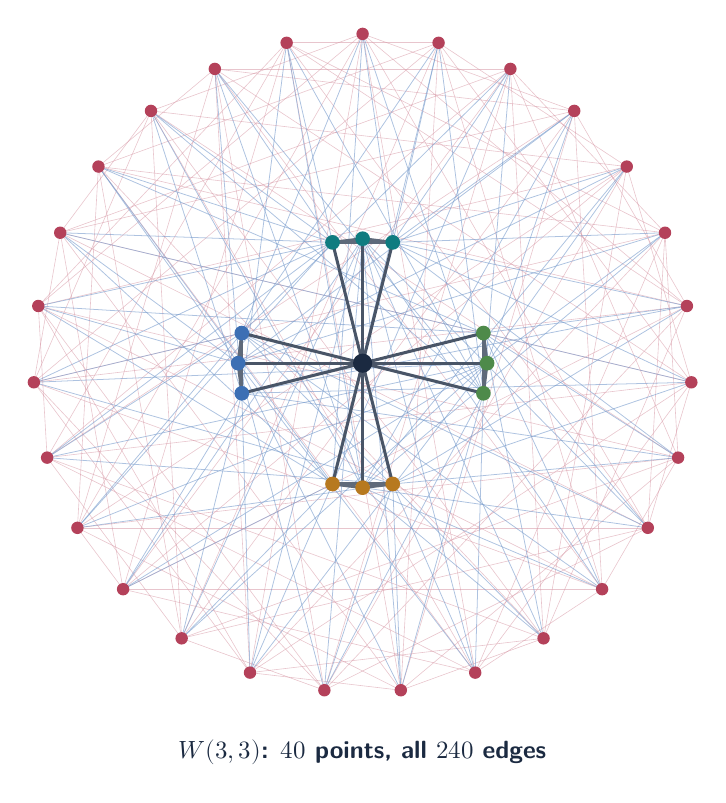
\begin{tikzpicture}[scale=1.02,
   ff/.style={rose!55,line width=0.22pt,opacity=0.55},
   nf/.style={sky!70,line width=0.28pt,opacity=0.6},
   nn/.style={ink!70,line width=1.1pt},
   pn/.style={ink!80,line width=1.1pt}]
  % generated by make_figures.py -- W(3,3), 40 points, 240 edges
\draw[ff] (0.000,4.100) -- (4.038,0.712);
\draw[ff] (0.000,4.100) -- (2.635,3.141);
\draw[ff] (0.000,4.100) -- (3.551,-2.050);
\draw[ff] (0.000,4.100) -- (-1.402,-3.853);
\draw[ff] (0.000,4.100) -- (1.402,-3.853);
\draw[ff] (0.000,4.100) -- (-3.551,-2.050);
\draw[ff] (4.038,0.712) -- (2.635,3.141);
\draw[ff] (4.038,0.712) -- (-4.093,-0.238);
\draw[ff] (4.038,0.712) -- (-0.946,3.989);
\draw[ff] (4.038,0.712) -- (-2.982,-2.814);
\draw[ff] (2.635,3.141) -- (-2.253,-3.426);
\draw[ff] (2.635,3.141) -- (0.476,-4.072);
\draw[ff] (2.635,3.141) -- (-3.928,-1.176);
\draw[ff] (2.635,3.141) -- (-3.765,1.624);
\draw[ff] (3.551,-2.050) -- (-3.551,-2.050);
\draw[ff] (3.551,-2.050) -- (4.093,-0.238);
\draw[ff] (3.551,-2.050) -- (-2.253,-3.426);
\draw[ff] (3.551,-2.050) -- (-3.765,1.624);
\draw[ff] (3.551,-2.050) -- (-0.946,3.989);
\draw[ff] (-1.402,-3.853) -- (4.093,-0.238);
\draw[ff] (-1.402,-3.853) -- (0.476,-4.072);
\draw[ff] (-1.402,-3.853) -- (-4.093,-0.238);
\draw[ff] (1.402,-3.853) -- (4.093,-0.238);
\draw[ff] (-4.038,0.712) -- (0.000,4.100);
\draw[ff] (-4.038,0.712) -- (-1.402,-3.853);
\draw[ff] (-4.038,0.712) -- (3.289,2.448);
\draw[ff] (-4.038,0.712) -- (3.928,-1.176);
\draw[ff] (-4.038,0.712) -- (2.982,-2.814);
\draw[ff] (-4.038,0.712) -- (-3.928,-1.176);
\draw[ff] (-4.038,0.712) -- (-0.946,3.989);
\draw[ff] (-4.038,0.712) -- (-0.476,-4.072);
\draw[ff] (-2.635,3.141) -- (0.000,4.100);
\draw[ff] (-2.635,3.141) -- (1.402,-3.853);
\draw[ff] (-2.635,3.141) -- (3.928,-1.176);
\draw[ff] (-2.635,3.141) -- (-2.253,-3.426);
\draw[ff] (-2.635,3.141) -- (-3.765,1.624);
\draw[ff] (-2.635,3.141) -- (-4.093,-0.238);
\draw[ff] (-2.635,3.141) -- (2.253,-3.426);
\draw[ff] (0.946,3.989) -- (4.093,-0.238);
\draw[ff] (0.946,3.989) -- (0.476,-4.072);
\draw[ff] (0.946,3.989) -- (-0.946,3.989);
\draw[ff] (3.289,2.448) -- (-3.551,-2.050);
\draw[ff] (3.289,2.448) -- (-2.635,3.141);
\draw[ff] (3.289,2.448) -- (0.946,3.989);
\draw[ff] (3.289,2.448) -- (4.093,-0.238);
\draw[ff] (3.289,2.448) -- (2.253,-3.426);
\draw[ff] (3.289,2.448) -- (-0.476,-4.072);
\draw[ff] (3.289,2.448) -- (-2.982,-2.814);
\draw[ff] (1.840,3.664) -- (3.765,1.624);
\draw[ff] (1.840,3.664) -- (3.928,-1.176);
\draw[ff] (1.840,3.664) -- (-3.928,-1.176);
\draw[ff] (1.840,3.664) -- (-3.765,1.624);
\draw[ff] (1.840,3.664) -- (2.253,-3.426);
\draw[ff] (1.840,3.664) -- (-0.476,-4.072);
\draw[ff] (1.840,3.664) -- (-2.982,-2.814);
\draw[ff] (3.765,1.624) -- (3.551,-2.050);
\draw[ff] (3.765,1.624) -- (-1.402,-3.853);
\draw[ff] (3.765,1.624) -- (1.402,-3.853);
\draw[ff] (3.765,1.624) -- (3.928,-1.176);
\draw[ff] (3.765,1.624) -- (-4.093,-0.238);
\draw[ff] (3.765,1.624) -- (-0.946,3.989);
\draw[ff] (3.928,-1.176) -- (-3.551,-2.050);
\draw[ff] (3.928,-1.176) -- (2.982,-2.814);
\draw[ff] (3.928,-1.176) -- (-2.253,-3.426);
\draw[ff] (3.928,-1.176) -- (0.476,-4.072);
\draw[ff] (2.982,-2.814) -- (2.635,3.141);
\draw[ff] (2.982,-2.814) -- (1.402,-3.853);
\draw[ff] (2.982,-2.814) -- (0.946,3.989);
\draw[ff] (2.982,-2.814) -- (-4.093,-0.238);
\draw[ff] (2.982,-2.814) -- (-2.982,-2.814);
\draw[ff] (-2.253,-3.426) -- (0.946,3.989);
\draw[ff] (-2.253,-3.426) -- (-3.928,-1.176);
\draw[ff] (0.476,-4.072) -- (-3.551,-2.050);
\draw[ff] (0.476,-4.072) -- (-3.765,1.624);
\draw[ff] (0.476,-4.072) -- (-0.946,3.989);
\draw[ff] (-3.928,-1.176) -- (1.402,-3.853);
\draw[ff] (-3.928,-1.176) -- (4.093,-0.238);
\draw[ff] (-3.928,-1.176) -- (-0.946,3.989);
\draw[ff] (-3.765,1.624) -- (4.093,-0.238);
\draw[ff] (-1.840,3.664) -- (2.635,3.141);
\draw[ff] (-1.840,3.664) -- (-1.402,-3.853);
\draw[ff] (-1.840,3.664) -- (-3.551,-2.050);
\draw[ff] (-1.840,3.664) -- (4.093,-0.238);
\draw[ff] (-1.840,3.664) -- (1.840,3.664);
\draw[ff] (-1.840,3.664) -- (2.982,-2.814);
\draw[ff] (-1.840,3.664) -- (-3.289,2.448);
\draw[ff] (-1.840,3.664) -- (-0.476,-4.072);
\draw[ff] (-4.093,-0.238) -- (0.946,3.989);
\draw[ff] (-4.093,-0.238) -- (-3.765,1.624);
\draw[ff] (-3.289,2.448) -- (4.038,0.712);
\draw[ff] (-3.289,2.448) -- (1.402,-3.853);
\draw[ff] (-3.289,2.448) -- (-3.551,-2.050);
\draw[ff] (-3.289,2.448) -- (0.946,3.989);
\draw[ff] (-3.289,2.448) -- (3.765,1.624);
\draw[ff] (-3.289,2.448) -- (-2.253,-3.426);
\draw[ff] (-3.289,2.448) -- (2.253,-3.426);
\draw[ff] (2.253,-3.426) -- (4.038,0.712);
\draw[ff] (2.253,-3.426) -- (-1.402,-3.853);
\draw[ff] (2.253,-3.426) -- (0.476,-4.072);
\draw[ff] (2.253,-3.426) -- (-3.928,-1.176);
\draw[ff] (-0.476,-4.072) -- (4.038,0.712);
\draw[ff] (-0.476,-4.072) -- (3.551,-2.050);
\draw[ff] (-0.476,-4.072) -- (-2.253,-3.426);
\draw[ff] (-0.476,-4.072) -- (-4.093,-0.238);
\draw[ff] (-2.982,-2.814) -- (1.402,-3.853);
\draw[ff] (-2.982,-2.814) -- (-3.551,-2.050);
\draw[ff] (-2.982,-2.814) -- (-3.765,1.624);
\draw[ff] (-2.982,-2.814) -- (-0.946,3.989);
\draw[nf] (0.375,1.504) -- (0.000,4.100);
\draw[nf] (0.375,1.504) -- (4.038,0.712);
\draw[nf] (0.375,1.504) -- (2.635,3.141);
\draw[nf] (0.375,1.504) -- (0.946,3.989);
\draw[nf] (0.375,1.504) -- (4.093,-0.238);
\draw[nf] (0.375,1.504) -- (3.289,2.448);
\draw[nf] (0.375,1.504) -- (1.840,3.664);
\draw[nf] (0.375,1.504) -- (3.765,1.624);
\draw[nf] (0.375,1.504) -- (3.928,-1.176);
\draw[nf] (0.000,4.100) -- (1.504,-0.375);
\draw[nf] (4.038,0.712) -- (1.504,0.375);
\draw[nf] (4.038,0.712) -- (0.375,-1.504);
\draw[nf] (-1.504,0.375) -- (0.000,4.100);
\draw[nf] (-1.504,0.375) -- (3.551,-2.050);
\draw[nf] (-1.504,0.375) -- (-3.551,-2.050);
\draw[nf] (-1.504,0.375) -- (0.946,3.989);
\draw[nf] (-1.504,0.375) -- (1.840,3.664);
\draw[nf] (-1.504,0.375) -- (2.982,-2.814);
\draw[nf] (-1.504,0.375) -- (-3.928,-1.176);
\draw[nf] (-1.504,0.375) -- (-4.093,-0.238);
\draw[nf] (-1.504,0.375) -- (2.253,-3.426);
\draw[nf] (-0.375,-1.504) -- (0.000,4.100);
\draw[nf] (-0.375,-1.504) -- (-1.402,-3.853);
\draw[nf] (-0.375,-1.504) -- (0.946,3.989);
\draw[nf] (-0.375,-1.504) -- (-2.253,-3.426);
\draw[nf] (-0.375,-1.504) -- (-3.765,1.624);
\draw[nf] (-0.375,-1.504) -- (-2.982,-2.814);
\draw[nf] (1.504,-0.375) -- (1.402,-3.853);
\draw[nf] (1.504,-0.375) -- (0.946,3.989);
\draw[nf] (1.504,-0.375) -- (0.476,-4.072);
\draw[nf] (1.504,-0.375) -- (-0.946,3.989);
\draw[nf] (-4.038,0.712) -- (-0.375,-1.504);
\draw[nf] (-4.038,0.712) -- (-0.375,1.504);
\draw[nf] (-4.038,0.712) -- (-1.550,0.000);
\draw[nf] (-4.038,0.712) -- (1.504,0.375);
\draw[nf] (-2.635,3.141) -- (1.504,-0.375);
\draw[nf] (-2.635,3.141) -- (-0.375,1.504);
\draw[nf] (-2.635,3.141) -- (-0.000,-1.550);
\draw[nf] (-2.635,3.141) -- (-1.504,-0.375);
\draw[nf] (0.000,1.550) -- (3.551,-2.050);
\draw[nf] (0.000,1.550) -- (-1.402,-3.853);
\draw[nf] (0.000,1.550) -- (1.402,-3.853);
\draw[nf] (0.000,1.550) -- (2.982,-2.814);
\draw[nf] (0.000,1.550) -- (-2.253,-3.426);
\draw[nf] (0.000,1.550) -- (0.476,-4.072);
\draw[nf] (0.000,1.550) -- (-2.982,-2.814);
\draw[nf] (-0.375,1.504) -- (-3.551,-2.050);
\draw[nf] (-0.375,1.504) -- (-3.928,-1.176);
\draw[nf] (-0.375,1.504) -- (-3.765,1.624);
\draw[nf] (-0.375,1.504) -- (-4.093,-0.238);
\draw[nf] (-0.375,1.504) -- (-0.946,3.989);
\draw[nf] (3.289,2.448) -- (-1.550,0.000);
\draw[nf] (3.289,2.448) -- (-0.000,-1.550);
\draw[nf] (3.289,2.448) -- (1.550,0.000);
\draw[nf] (1.840,3.664) -- (-0.375,-1.504);
\draw[nf] (1.840,3.664) -- (1.504,-0.375);
\draw[nf] (3.765,1.624) -- (-0.000,-1.550);
\draw[nf] (3.765,1.624) -- (1.550,0.000);
\draw[nf] (3.928,-1.176) -- (1.504,0.375);
\draw[nf] (3.928,-1.176) -- (0.375,-1.504);
\draw[nf] (-1.550,0.000) -- (2.635,3.141);
\draw[nf] (-1.550,0.000) -- (1.402,-3.853);
\draw[nf] (-1.550,0.000) -- (3.765,1.624);
\draw[nf] (-1.550,0.000) -- (0.476,-4.072);
\draw[nf] (-1.550,0.000) -- (-3.765,1.624);
\draw[nf] (-1.550,0.000) -- (-3.289,2.448);
\draw[nf] (-1.550,0.000) -- (-0.476,-4.072);
\draw[nf] (-0.000,-1.550) -- (2.635,3.141);
\draw[nf] (-0.000,-1.550) -- (3.551,-2.050);
\draw[nf] (-0.000,-1.550) -- (2.982,-2.814);
\draw[nf] (-0.000,-1.550) -- (-0.946,3.989);
\draw[nf] (1.550,0.000) -- (2.635,3.141);
\draw[nf] (1.550,0.000) -- (-1.402,-3.853);
\draw[nf] (1.550,0.000) -- (-3.551,-2.050);
\draw[nf] (1.550,0.000) -- (-2.253,-3.426);
\draw[nf] (1.550,0.000) -- (-3.928,-1.176);
\draw[nf] (1.550,0.000) -- (-4.093,-0.238);
\draw[nf] (1.550,0.000) -- (-2.982,-2.814);
\draw[nf] (2.982,-2.814) -- (1.504,0.375);
\draw[nf] (-1.840,3.664) -- (1.504,-0.375);
\draw[nf] (-1.840,3.664) -- (-0.375,1.504);
\draw[nf] (-1.840,3.664) -- (-0.000,-1.550);
\draw[nf] (-1.840,3.664) -- (-1.504,-0.375);
\draw[nf] (-1.504,-0.375) -- (4.038,0.712);
\draw[nf] (-1.504,-0.375) -- (-1.402,-3.853);
\draw[nf] (-1.504,-0.375) -- (4.093,-0.238);
\draw[nf] (-1.504,-0.375) -- (3.928,-1.176);
\draw[nf] (-1.504,-0.375) -- (-2.253,-3.426);
\draw[nf] (-1.504,-0.375) -- (-0.946,3.989);
\draw[nf] (-1.504,-0.375) -- (-2.982,-2.814);
\draw[nf] (1.504,0.375) -- (3.551,-2.050);
\draw[nf] (1.504,0.375) -- (4.093,-0.238);
\draw[nf] (1.504,0.375) -- (-3.765,1.624);
\draw[nf] (0.375,-1.504) -- (1.402,-3.853);
\draw[nf] (0.375,-1.504) -- (-3.551,-2.050);
\draw[nf] (0.375,-1.504) -- (4.093,-0.238);
\draw[nf] (0.375,-1.504) -- (0.476,-4.072);
\draw[nf] (0.375,-1.504) -- (-3.928,-1.176);
\draw[nf] (0.375,-1.504) -- (-4.093,-0.238);
\draw[nf] (-3.289,2.448) -- (-0.375,-1.504);
\draw[nf] (-3.289,2.448) -- (-0.375,1.504);
\draw[nf] (-3.289,2.448) -- (1.504,0.375);
\draw[nf] (2.253,-3.426) -- (0.000,1.550);
\draw[nf] (2.253,-3.426) -- (-0.000,-1.550);
\draw[nf] (2.253,-3.426) -- (1.504,0.375);
\draw[nf] (-0.476,-4.072) -- (1.504,-0.375);
\draw[nf] (-0.476,-4.072) -- (0.000,1.550);
\draw[nf] (-0.476,-4.072) -- (0.375,-1.504);
\draw[nn] (0.375,1.504) -- (0.000,1.550);
\draw[nn] (0.375,1.504) -- (-0.375,1.504);
\draw[nn] (-1.504,0.375) -- (-1.504,-0.375);
\draw[nn] (-0.375,-1.504) -- (-0.000,-1.550);
\draw[nn] (-0.375,-1.504) -- (0.375,-1.504);
\draw[nn] (1.504,-0.375) -- (1.550,0.000);
\draw[nn] (1.504,-0.375) -- (1.504,0.375);
\draw[nn] (0.000,1.550) -- (-0.375,1.504);
\draw[nn] (-1.550,0.000) -- (-1.504,0.375);
\draw[nn] (-1.550,0.000) -- (-1.504,-0.375);
\draw[nn] (-0.000,-1.550) -- (0.375,-1.504);
\draw[nn] (1.550,0.000) -- (1.504,0.375);
\draw[pn] (0.375,1.504) -- (0.000,0.000);
\draw[pn] (-1.504,0.375) -- (0.000,0.000);
\draw[pn] (-0.375,-1.504) -- (0.000,0.000);
\draw[pn] (0.000,0.000) -- (1.504,-0.375);
\draw[pn] (0.000,0.000) -- (0.000,1.550);
\draw[pn] (0.000,0.000) -- (-0.375,1.504);
\draw[pn] (0.000,0.000) -- (-0.000,-1.550);
\draw[pn] (0.000,0.000) -- (1.550,0.000);
\draw[pn] (0.000,0.000) -- (-1.504,-0.375);
\draw[pn] (0.000,0.000) -- (1.504,0.375);
\draw[pn] (0.000,0.000) -- (0.375,-1.504);
\draw[pn] (-1.550,0.000) -- (0.000,0.000);
\fill[teal] (0.375,1.504) circle (2.6pt);
\fill[teal] (0.000,1.550) circle (2.6pt);
\fill[teal] (-0.375,1.504) circle (2.6pt);
\fill[sky] (-1.504,0.375) circle (2.6pt);
\fill[sky] (-1.550,0.000) circle (2.6pt);
\fill[sky] (-1.504,-0.375) circle (2.6pt);
\fill[gold] (-0.375,-1.504) circle (2.6pt);
\fill[gold] (-0.000,-1.550) circle (2.6pt);
\fill[gold] (0.375,-1.504) circle (2.6pt);
\fill[sage] (1.504,-0.375) circle (2.6pt);
\fill[sage] (1.550,0.000) circle (2.6pt);
\fill[sage] (1.504,0.375) circle (2.6pt);
\fill[rose] (0.000,4.100) circle (2.2pt);
\fill[rose] (0.946,3.989) circle (2.2pt);
\fill[rose] (1.840,3.664) circle (2.2pt);
\fill[rose] (2.635,3.141) circle (2.2pt);
\fill[rose] (3.289,2.448) circle (2.2pt);
\fill[rose] (3.765,1.624) circle (2.2pt);
\fill[rose] (4.038,0.712) circle (2.2pt);
\fill[rose] (4.093,-0.238) circle (2.2pt);
\fill[rose] (3.928,-1.176) circle (2.2pt);
\fill[rose] (3.551,-2.050) circle (2.2pt);
\fill[rose] (2.982,-2.814) circle (2.2pt);
\fill[rose] (2.253,-3.426) circle (2.2pt);
\fill[rose] (1.402,-3.853) circle (2.2pt);
\fill[rose] (0.476,-4.072) circle (2.2pt);
\fill[rose] (-0.476,-4.072) circle (2.2pt);
\fill[rose] (-1.402,-3.853) circle (2.2pt);
\fill[rose] (-2.253,-3.426) circle (2.2pt);
\fill[rose] (-2.982,-2.814) circle (2.2pt);
\fill[rose] (-3.551,-2.050) circle (2.2pt);
\fill[rose] (-3.928,-1.176) circle (2.2pt);
\fill[rose] (-4.093,-0.238) circle (2.2pt);
\fill[rose] (-4.038,0.712) circle (2.2pt);
\fill[rose] (-3.765,1.624) circle (2.2pt);
\fill[rose] (-3.289,2.448) circle (2.2pt);
\fill[rose] (-2.635,3.141) circle (2.2pt);
\fill[rose] (-1.840,3.664) circle (2.2pt);
\fill[rose] (-0.946,3.989) circle (2.2pt);
\fill[ink] (0,0) circle (3.4pt);

  \node[font=\sffamily\small\bfseries,text=ink] at (0,-4.85) {$W(3,3)$: $40$ points, all $240$ edges};
\end{tikzpicture}

\medskip
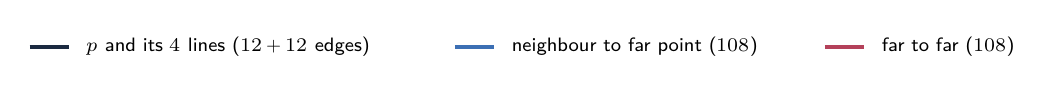
\begin{tikzpicture}
  \foreach \c/\t/\x in {ink/{$p$ and its $4$ lines ($12+12$ edges)}/0,
                        sky/{neighbour to far point ($108$)}/5.4,
                        rose/{far to far ($108$)}/10.1}{
    \draw[\c,line width=1.4pt] (\x,0) -- (\x+0.5,0);
    \node[anchor=west,font=\sffamily\scriptsize] at (\x+0.6,0) {\t};}
\end{tikzpicture}
\caption{A portrait of $\W$, computed from the symplectic form and drawn from the point
of view of one point $p$ (centre). Its $12$ neighbours lie on four lines (four colours,
three points each); the $27$ far points sit on the outer ring, ordered by which neighbour
they see on each of the four lines --- by the quadrangle axiom every far point sees exactly
one. The edge counts $12+12+108+108=240$ are forced by $\SRG(40,12,2,4)$.}
\label{fig:portrait}
\end{figure}

\begin{plainwords}
``Strongly regular'' means that the geometry looks exactly the same from every point, and
from every pair of points. There is no privileged measurement. The three eigenvalues are
the geometry's ``vibration frequencies''; that there are only three is the algebraic
signature of this perfect evenness.
\end{plainwords}

\subsection{What the points and lines are physically}

Let $W(x)=X^{x_1}Z^{x_3}\otimes X^{x_2}Z^{x_4}$ be the two-qutrit Pauli operator with
label $x\in\F_3^4$. A direct calculation from $ZX=\omega XZ$ gives
\begin{equation}\label{eq:commutation}
W(x)\,W(y)\;=\;\omega^{\langle x,y\rangle}\,W(y)\,W(x).
\end{equation}
So the symplectic form is not an arbitrary choice: it \emph{is} the commutation phase of
two-qutrit measurements.

\begin{physical}[What it means physically: contexts]
\begin{itemize}[leftmargin=1.2em]
\item A \textbf{point} is a measurement direction: the cyclic group generated by one
      Pauli operator, which is the same whether it is run forwards or backwards.
\item Two points are \textbf{collinear} when their operators commute and can be measured
      at the same time without disturbing each other.
\item A \textbf{line} is a maximal set of mutually compatible measurements: an abelian
      group of $9$ Pauli operators whose common eigenvectors form a basis of the
      two-qutrit space $\C^9$. Physicists call this a \emph{stabilizer group}, and each
      of its $9$ joint eigenstates a \emph{stabilizer state}. There are $40$ lines and
      so $40\times9=360$ stabilizer states --- the standard count for two qutrits.
\item The \textbf{quadrangle axiom} says: given any measurement and any complete
      measurement context not containing it, exactly one member of the context is
      compatible with it.
\end{itemize}
\end{physical}

The quantum operations that map Pauli operators to Pauli operators (up to phase) form the
two-qutrit \emph{Clifford group} \cite{GHW}. Modulo the Paulis themselves and phases, it acts on the
labels $x$ by exactly the linear maps preserving $\langle\,,\rangle$: the symplectic
group $\Sp(4,3)$. So the symmetries of the geometry are, literally, the ``cheap'' quantum
gates.

\subsection{Two groups of order 51,840, which are not the same group}

The symmetry groups that appear around $\W$ are easy to confuse, and confusing them has
cost this programme real work (Section~\ref{sec:e8-trap}). Adapting the blueprint's
account:
\[
\PSp(4,3)\cong U_4(2)\ (\text{order }25\,920),\qquad
\Sp(4,3)\cong 2.U_4(2),\qquad
\PGSp(4,3)\cong U_4(2){:}2\cong W(E_6).
\]
The last two both have order $51\,840$ but are \emph{not isomorphic}: $\Sp(4,3)$ has a
centre of order two (the map $x\mapsto -x$), while $\PGSp(4,3)$ --- the full automorphism
group of $\W$ --- has trivial centre and is the Weyl group of the exceptional root system
$E_6$. \tierT

\begin{plainwords}
The two groups have the same size but different ``shapes''. One of them contains a
special element that commutes with everything --- a global sign flip. Whether that sign
is visible or invisible turns out to decide whether the structure can tell left from
right. This is why the same forty points can \emph{host} a handedness without being able
to \emph{choose} one (Section~\ref{sec:chirality}).
\end{plainwords}

\subsection{The dual picture and a firewall}

Swap the roles of points and lines: the $40$ lines of $\W$, with two lines ``adjacent''
when they meet, form the dual quadrangle, which is the parabolic quadric $Q(4,3)$. For odd
$q$ the quadrangle $W(3,q)$ is \emph{not} isomorphic to its dual, although both have
collinearity graph parameters $\SRG(40,12,2,4)$. This distinction matters several times
below: the finite space-time of Section~4 lives on the \emph{line} side, while the
qutrit operators live on the \emph{point} side. Repeated coincidences of counts between the
two sides (for instance $27$ vertices, $108$ edges, $36$ triangles) do not make them the
same object --- the repository calls this the \emph{point/line firewall}, and it has
caught several tempting mistakes. \tierC\ (\cert{w33\_20260924\_history\_pointline\_cospectral\_firewall.py})

\subsection{Why three?}

A sceptical reader should ask whether ``three'' was chosen because it works. The
repository records five equations in which $q$ appears as an unknown integer and each has
exactly one positive solution, $q=3$. Two can be checked by hand:
\begin{itemize}
\item The number of edges of the collinearity graph of $W(3,q)$ is
      $q(q+1)^2(q^2+1)/2$; the number of elements of $\F_{q^5}$ outside $\F_q$ is $q^5-q$.
      Setting them equal gives $2(q-1)=q+1$, so $q=3$: both equal $240$.
\item The number of points not collinear with a given point is $q^3$; it equals $27$,
      the dimension of the fundamental representation of $E_6$, only for $q=3$.
\end{itemize}

\begin{boundary}
These are coincidences of integers, not derivations. They do not prove that three is
\emph{necessary} for anything physical. They do show that the programme's most unusual
choice --- three-level systems rather than two-level ones --- is the one value at which
several independent structures meet. \tierB
\end{boundary}

\section{One qutrit, acting on itself}
\label{sec:self}

Section~2 built $\W$ from \emph{two} qutrits. This section shows that one is enough ---
provided we look not at the qutrit's states but at the things that can be done to it.
That shift of viewpoint is the precise content of the phrase the Holonet papers use,
\emph{self-entanglement}, and it is worth getting exactly right, because the phrase can
also be read in ways that are not true.

\subsection{Operators are states}

An operator on one qutrit is a $3\times3$ matrix: nine complex numbers. So the space of
operators $\End(\C^3)$ is itself a nine-dimensional complex vector space, and with the
Hilbert--Schmidt inner product $\langle A,B\rangle=\tr(A^\dagger B)$ it is a Hilbert
space. Writing $\ket{A}\!\rangle$ for a matrix regarded as a vector,
\[
\End(\C^3)\;\cong\;\C^3\otimes\C^{3*}\;\cong\;\C^9,
\qquad
\ket{i}\!\bra{j}\;\longleftrightarrow\;\ket{i}\otimes\ket{j}.
\]
Under this identification the identity matrix becomes the maximally entangled
``Bell'' state of two qutrits,
\[
\ket{\Omega}=\tfrac{1}{\sqrt3}\ket{I}\!\rangle=\tfrac1{\sqrt3}\bigl(\ket{00}+\ket{11}+\ket{22}\bigr).
\]
This is the Choi--Jamio{\l}kowski correspondence, a standard tool of quantum information:
every operation on a system is encoded by a state of two copies of it.

\begin{plainwords}
Imagine describing a machine not by its current setting but by its complete instruction
table: ``if the input is $j$, produce $i$ with amplitude $A_{ij}$''. That table has nine
entries. The nine entries behave exactly like the state of two three-way systems --- an
``input'' and an ``output''. Nothing mystical is happening; it is the same information
written in a different shape. The ``two qutrits'' of Section~2 can be read as the
before-and-after of a single qutrit.
\end{plainwords}

\subsection{The two-sided action and its geometry}

Let $P_u=X^{u_1}Z^{u_2}$ for $u\in\F_3^2$. A qutrit operator $A$ can be multiplied by
Pauli operators from the left and from the right:
\[
\Phi_{u,v}(A)=P_u\,A\,P_v^\dagger ,\qquad (u,v)\in\F_3^2\oplus\F_3^2 .
\]

\begin{result}{Theorem 3.1 \hfill \tierT\ \tierC}
The $81$ maps $\Phi_{u,v}$ form an orthogonal basis of $\End(\End(\C^3))\cong M_9(\C)$;
the $80$ non-identity maps span $\sll_9$. They commute up to the phase
\[
\Phi_{u,v}\Phi_{u',v'}=\omega^{[u,u']-[v,v']}\,\Phi_{u',v'}\Phi_{u,v},
\qquad [u,u']=u_1u'_2-u_2u'_1 .
\]
The form $[u,u']-[v,v']$ is symplectic on $\F_3^4$, and the resulting commutation
geometry on the $40$ projective classes is $\W$, with collinearity graph
$\SRG(40,12,2,4)$ and spectrum $12^1\,2^{24}\,(-4)^{15}$.
\cert{w33\_20260924\_temporal\_su9\_e8\_compiler.py}
\end{result}

\begin{proof}[Proof of the phase]
$\Phi_{u,v}\Phi_{u',v'}(A)=P_uP_{u'}AP_{v'}^\dagger P_v^\dagger$ and
$\Phi_{u',v'}\Phi_{u,v}(A)=P_{u'}P_uAP_v^\dagger P_{v'}^\dagger$. Using
$P_uP_{u'}=\omega^{[u,u']}P_{u'}P_u$ and taking adjoints of
$P_vP_{v'}=\omega^{[v,v']}P_{v'}P_v$ gives the ratio $\omega^{[u,u']-[v,v']}$.
\end{proof}

The minus sign is the fingerprint of right multiplication: acting from the right reverses
the order of products, so the right-hand copy of the qutrit carries the \emph{opposite}
algebra. The two ``qutrits'' are not two particles, and not even two subsystems in the
usual sense: they are the algebra of left actions and its commutant, the algebra of right
actions, on one qutrit's operator space.

\subsection{The Bell line is the set of physical channels}

Among all $\Phi_{u,v}$, which ones are genuine quantum operations? A linear map on
operators is physically realisable as a quantum channel only if it is \emph{completely
positive}, which for $\Phi_{u,v}$ means its Choi matrix
$\ket{P_u}\!\rangle\langle\!\bra{P_v}$ is positive semidefinite. A rank-one matrix
$\ket{a}\bra{b}$ is positive only when $b$ is a positive multiple of $a$; so up to phase,
$\Phi_{u,v}$ is completely positive exactly when $u=v$. The diagonal
$\Delta=\{(u,u)\}$ is totally isotropic ($[u,u']-[u,u']=0$) and its four projective points
form one line of $\W$.

\begin{result}{Proposition 3.2 \hfill \tierT\ \tierC}
The unitary channels $A\mapsto P_uAP_u^\dagger$ form a distinguished line of $\W$, the
\emph{Bell line}; each fixes $\ket{\Omega}$. The left--right exchange
$(u,v)\mapsto(v,u)$ reverses the symplectic form; its eight fixed rays split into two
Lagrangian lines, and the $+$ line is exactly the unitary-channel diagonal.
\cert{w33\_20260924\_liouville\_swap\_cp\_outer\_bridge.py}
\end{result}

\begin{physical}[What it means physically: a built-in time reversal]
Exchanging left and right multiplication is the operator version of running a process
backwards: $A\mapsto P_uAP_v^\dagger$ becomes $A\mapsto P_vAP_u^\dagger$. Because it
reverses the sign of the commutation form, it is an \emph{anti}-symmetry of $\W$ --- the
same kind of map as complex conjugation, which is how quantum mechanics implements time
reversal. The repository shows that ordinary matrix transposition of the Pauli algebra
induces exactly this class of outer symmetry, the one earlier work had identified
abstractly (BT172). \tierC\ (\cert{w33\_20260924\_intrinsic\_transpose\_outer.py}, up to a
labelling gauge.)
\end{physical}

\subsection{Three different things called ``self-entanglement''}

The phrase can mean three distinct things, and the Holonet programme has, at times, slid
between them. It is worth separating them once and for all.

\begin{center}
\small
\renewcommand{\arraystretch}{1.3}
\begin{tabularx}{\textwidth}{@{}p{3.1cm}Xp{3.6cm}@{}}
\toprule
\textbf{Notion} & \textbf{What is entangled} & \textbf{Status here}\\
\midrule
Intraparticle & Two independent degrees of freedom of one photon (for example its
arrival-time bin and its frequency bin). & Standard and experimentally demonstrated.\\
Operator (Choi) & The input and output legs of one operation, as in \S3.1. & The exact
algebraic home of $\W$.\\
Temporal process & Quantum correlations between interventions at different times,
described by a multi-time \emph{process tensor}. & Needs its own witness (\S3.5).\\
\bottomrule
\end{tabularx}
\end{center}

\begin{boundary}[A correction the papers needed]
An earlier draft of the photonic paper described three optical time bins as containing
``a past qutrit and a future qutrit''. Three orthogonal bins span only $\C^3$, whereas two
qutrits need $\C^9$; the two-bin subsets it named overlap and cannot be independent tensor
factors. The architecture now uses two genuinely independent qutrit degrees of freedom
of one photon --- time bin $\otimes$ frequency bin --- and reads ``past'' and ``future''
as the input and output legs of a process, not as simultaneously existing copies.
\tierX\ (the three-bin reading) \quad \tierT\ (the corrected encoding).
\end{boundary}

\subsection{Memory across a causal break}

What does it take for a system to carry quantum information from one time to a later
one? The repository's cleanest test is a three-step process with a qutrit memory $M$:
swap the system $S$ into $M$; discard $S$ and replace it with anything at all (a
\emph{causal break}); swap back. If the original state reappears, the process had
memory. But a classical memory that merely records ``$0$, $1$ or $2$'' would pass that
test too. The decisive witness entangles $S$ with a reference $R$ first.

\begin{result}{Theorem 3.3 \hfill \tierC}
With $S$ initially maximally entangled with a reference qutrit $R$:
\begin{itemize}
\item a coherent memory returns the Bell state exactly (negativity $1$, Bell fidelity $1$);
\item a classical label memory returns $\tfrac13\sum_j\ket{jj}\!\bra{jj}$ (negativity $0$,
      Bell fidelity $\tfrac13$), although it passes every basis-state retrieval test;
\item a depolarizing memory $\rho\mapsto(1-p)\rho+p\,I/3$ returns an isotropic state with
      Bell fidelity $1-\tfrac{8p}{9}$ and negativity $\max\bigl(0,\tfrac{3-4p}{3}\bigr)$;
      quantum memory survives exactly while $p<\tfrac34$.
\end{itemize}
\cert{w33\_20260924\_temporal\_quantum\_memory\_witness.json}
\end{result}

\begin{physical}
The threshold $p=\tfrac34$ is the standard point at which a qutrit depolarizing channel
becomes entanglement-breaking: beyond it, the link between the earlier and the later
system can still carry classical information but no longer quantum information. Retrieval
after a break proves that the past is \emph{remembered}; preserved entanglement with a
reference proves that it is remembered \emph{quantumly}. Neither involves any influence
travelling backwards in time.
\end{physical}

\subsection{A state picks a clock}

A faithful qutrit state $\rho=\mathrm{diag}(p_0,p_1,p_2)$ defines a natural flow on
operators, the \emph{modular flow} of Tomita--Takesaki theory, with generator
$K=-\log\rho\otimes1+1\otimes\log\rho$ acting on $\End(\C^3)$. The matrix units are its
eigenvectors:
\[
K\,E_{ij}=\log\!\frac{p_j}{p_i}\,E_{ij}.
\]
The three diagonal units have frequency zero; the six off-diagonal units $E_{ij}$
($i\neq j$) --- the six directed transitions between the three levels --- come in three
opposite pairs. Their pattern of differences is exactly the root system $A_2$.
\tierC\ (\cert{w33\_20260924\_modular\_a2\_event\_clock.py})

\begin{plainwords}
A perfectly balanced qutrit ($p_0=p_1=p_2$) has no preferred direction: every transition
has zero frequency, and nothing distinguishes ``forward'' from ``backward''. Any imbalance
gives each of the six transitions a frequency, and pairs each with its reverse at the
opposite frequency. This is the finite form of an old idea of Connes and Rovelli \cite{ConnesRovelli}: that a
state of a system can itself define a flow of time. It orients change; it does not by
itself make change irreversible. That distinction --- between an orientation of time and
an arrow of time --- returns in Section~4.
\end{plainwords}

\section{Time: a finite light cone and four clocks}
\label{sec:time}

Section~3 ended with a qutrit whose operators behave like the before-and-after of a
process. This section asks what \emph{time} looks like inside $\W$. The answer comes in
three layers, and keeping them apart is the main lesson of the section:
\begin{enumerate}[label=\textbf{\arabic*.},leftmargin=1.6em]
\item a finite \textbf{present}: $27$ ``events'' carrying an exact Minkowski-type form
      $t^2-x^2-y^2$, with a light cone and four null directions;
\item an unbounded \textbf{history}: the paths through those events, which never close up
      and which remember a winding number that the present forgets;
\item an \textbf{arrow}: the direction of time in the thermodynamic sense, which appears
      only when information is thrown away.
\end{enumerate}
Everything in layers 1 and 2 is reversible. Layer 3 is where irreversibility enters, and
we shall see exactly what it costs.

% ------------------------------------------------------------------
\subsection{Choosing a ``now''}

Fix one line $B$ of $\W$ --- the Bell line of Section~3, the unitary channels. The other
$39$ lines fall into two kinds: $12$ lines meet $B$ (three through each of its four
points), and $27$ lines miss it entirely. Every line that misses $B$ can be written
uniquely as
\[
L_S=\{(Sy,\,y)\;:\;y\in\F_3^2\},\qquad S=\begin{pmatrix}a&b\\ b&c\end{pmatrix},\quad a,b,c\in\F_3 ,
\]
for a \emph{symmetric} $2\times2$ matrix $S$. There are $3^3=27$ such matrices. So the
lines of $\W$ decompose as
\[
40\;=\;\underbrace{1}_{B}\;+\;\underbrace{12}_{\text{meet }B}\;+\;\underbrace{27}_{\text{histories } S}.
\]

\begin{figure}[htbp]
\centering
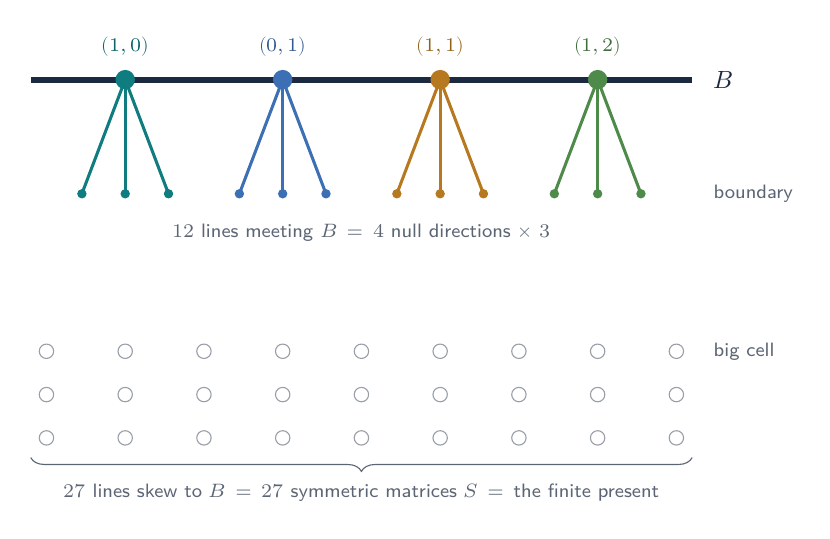
\begin{tikzpicture}[scale=1.0,
   bp/.style={circle,fill=#1,inner sep=0pt,minimum size=7pt},
   hist/.style={circle,draw=ink!45,fill=white,inner sep=0pt,minimum size=5.2pt}]
  % Bell line
  \draw[ink,line width=2.2pt] (-4.2,3.2) -- (4.2,3.2);
  \node[font=\sffamily\small\bfseries,text=ink,anchor=west] at (4.35,3.2) {$B$};
  \foreach \x/\c/\lab in {-3/teal/{(1,0)},-1/sky/{(0,1)},1/gold/{(1,1)},3/sage/{(1,2)}}{
    \node[bp=\c] (b\x) at (\x,3.2) {};
    \node[font=\scriptsize,text=\c!80!black] at (\x,3.62) {$\lab$};
    \foreach \d in {-0.55,0,0.55}{
      \draw[\c,line width=1.1pt] (\x,3.2) -- (\x+\d,1.75);
      \fill[\c] (\x+\d,1.75) circle (1.7pt);}
  }
  \node[font=\sffamily\scriptsize,text=slate,align=center] at (0,1.25)
     {$12$ lines meeting $B$ \,=\, $4$ null directions $\times$ $3$};
  % 27 histories
  \begin{scope}[yshift=-0.55cm]
  \foreach \i in {0,...,26}{
     \pgfmathsetmacro{\xx}{-4.0+ (mod(\i,9))*1.0}
     \pgfmathsetmacro{\yy}{0.3-floor(\i/9)*0.55}
     \node[hist] at (\xx,\yy) {};}
  \draw[decorate,decoration={brace,amplitude=5pt,mirror},slate] (-4.2,-1.05) -- (4.2,-1.05);
  \node[font=\sffamily\scriptsize,text=slate] at (0,-1.5)
     {$27$ lines skew to $B$ \,=\, $27$ symmetric matrices $S$ \,=\, the finite present};
  \end{scope}
  \node[font=\sffamily\scriptsize,text=slate,anchor=west] at (4.35,1.75) {boundary};
  \node[font=\sffamily\scriptsize,text=slate,anchor=west] at (4.35,-0.25) {big cell};
\end{tikzpicture}
\caption{The forty lines of $\W$ seen from the Bell line $B$. The four points of $B$
are labelled by the four projective directions of $\F_3^2$; they will turn out to be the
four null directions of a finite light cone. The $1+12=13$ lines touching $B$ form the
``boundary''; the $27$ others are the events of the finite present.}
\label{fig:bellview}
\end{figure}

The $13$ boundary lines are not an arbitrary leftover. In Pl\"ucker coordinates the $40$
lines of $\W$ lie on the quadric $x_0x_4-x_1x_3+x_2^2=0$ in $\mathbb{P}^4(\F_3)$ ---
this is the dual quadrangle $Q(4,3)$ of Section~2 --- and the $27$ histories are its
``big cell'' $x_0\neq0$, reached by $S\mapsto[1:a:b:c:ac-b^2]$. The $13$ points with
$x_0=0$ form the tangent cone of the quadric at $B$: $B$ itself plus four three-point
generators, one for each point of $B$. \tierC\ (\cert{w33\_20260924\_history\_bigcell\_q43\_compactification.py})

% ------------------------------------------------------------------
\subsection{The finite light cone}

Two histories $L_S$ and $L_T$ are either disjoint or they meet in a point. A short
calculation shows they meet exactly when
\[
\det(S-T)=0 .
\]
Write $S=\begin{pmatrix} t+x & y\\ y & t-x\end{pmatrix}$ (possible because $2$ is
invertible mod $3$). Then
\[
\boxed{\;\det S \;=\; t^2-x^2-y^2\;}
\]
--- the Minkowski form of a space-time with one time and two space dimensions. Two events
are \emph{null-separated} (``light can travel between them'') exactly when their lines
meet, i.e.\ when the two contexts share a measurement.

\begin{result}{Theorem 4.1 \hfill \tierT\ \tierC}
The $27$ histories form the finite Minkowski space $(\F_3^3,\;t^2-x^2-y^2)$. Relative to any
event, the other $26$ split as $8$ null, $6$ timelike ($\det=1$) and $12$ spacelike
($\det=-1$). The null directions through an event are the four rank-one matrices
$vv^{\mathsf T}$, $v\in\mathbb{P}^1(\F_3)$, and they correspond bijectively to the four
points of $B$.
\cert{w33\_20260924\_history\_bigcell\_q43\_compactification.py}
\end{result}

\begin{figure}[htbp]
\centering
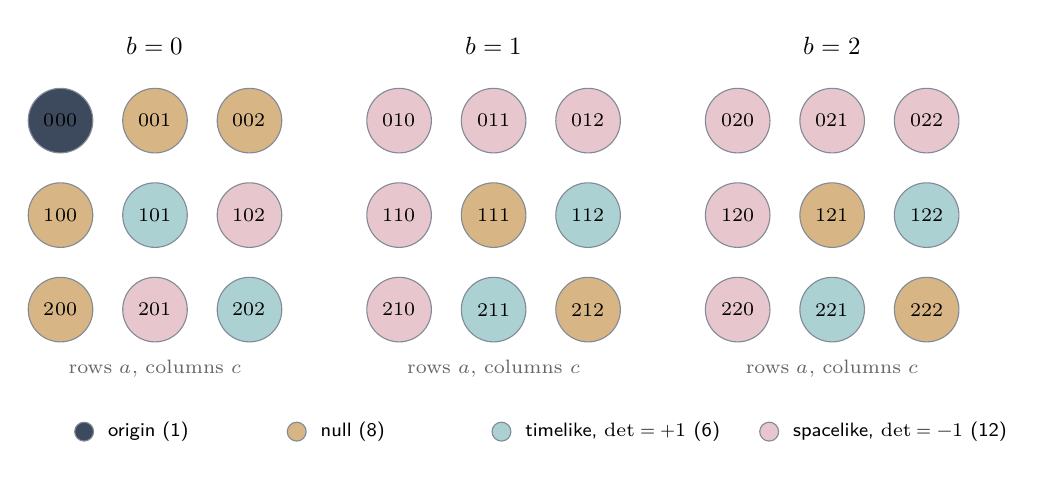
\begin{tikzpicture}[ev/.style={circle,draw=ink!55,line width=0.4pt,minimum size=8.2mm,inner sep=0pt}]
\node[font=\small] at (1.20,3.35) {$b=0$};
\node[ev,fill=orgn] at (0.00,2.40) {$\scriptstyle 000$};
\node[ev,fill=nullc] at (1.20,2.40) {$\scriptstyle 001$};
\node[ev,fill=nullc] at (2.40,2.40) {$\scriptstyle 002$};
\node[ev,fill=nullc] at (0.00,1.20) {$\scriptstyle 100$};
\node[ev,fill=plusc] at (1.20,1.20) {$\scriptstyle 101$};
\node[ev,fill=minusc] at (2.40,1.20) {$\scriptstyle 102$};
\node[ev,fill=nullc] at (0.00,0.00) {$\scriptstyle 200$};
\node[ev,fill=minusc] at (1.20,0.00) {$\scriptstyle 201$};
\node[ev,fill=plusc] at (2.40,0.00) {$\scriptstyle 202$};
\node[font=\scriptsize,text=black!60] at (1.20,-0.75) {rows $a$, columns $c$};
\node[font=\small] at (5.50,3.35) {$b=1$};
\node[ev,fill=minusc] at (4.30,2.40) {$\scriptstyle 010$};
\node[ev,fill=minusc] at (5.50,2.40) {$\scriptstyle 011$};
\node[ev,fill=minusc] at (6.70,2.40) {$\scriptstyle 012$};
\node[ev,fill=minusc] at (4.30,1.20) {$\scriptstyle 110$};
\node[ev,fill=nullc] at (5.50,1.20) {$\scriptstyle 111$};
\node[ev,fill=plusc] at (6.70,1.20) {$\scriptstyle 112$};
\node[ev,fill=minusc] at (4.30,0.00) {$\scriptstyle 210$};
\node[ev,fill=plusc] at (5.50,0.00) {$\scriptstyle 211$};
\node[ev,fill=nullc] at (6.70,0.00) {$\scriptstyle 212$};
\node[font=\scriptsize,text=black!60] at (5.50,-0.75) {rows $a$, columns $c$};
\node[font=\small] at (9.80,3.35) {$b=2$};
\node[ev,fill=minusc] at (8.60,2.40) {$\scriptstyle 020$};
\node[ev,fill=minusc] at (9.80,2.40) {$\scriptstyle 021$};
\node[ev,fill=minusc] at (11.00,2.40) {$\scriptstyle 022$};
\node[ev,fill=minusc] at (8.60,1.20) {$\scriptstyle 120$};
\node[ev,fill=nullc] at (9.80,1.20) {$\scriptstyle 121$};
\node[ev,fill=plusc] at (11.00,1.20) {$\scriptstyle 122$};
\node[ev,fill=minusc] at (8.60,0.00) {$\scriptstyle 220$};
\node[ev,fill=plusc] at (9.80,0.00) {$\scriptstyle 221$};
\node[ev,fill=nullc] at (11.00,0.00) {$\scriptstyle 222$};
\node[font=\scriptsize,text=black!60] at (9.80,-0.75) {rows $a$, columns $c$};

\begin{scope}[yshift=-1.55cm]
 \foreach \c/\t/\x in {orgn/{origin (1)}/0.3,nullc/{null (8)}/3.0,plusc/{timelike, $\det=+1$ (6)}/5.6,minusc/{spacelike, $\det=-1$ (12)}/9.0}{
   \fill[\c,draw=ink!55] (\x,0) circle (1.2mm);
   \node[anchor=west,font=\sffamily\scriptsize] at (\x+0.18,0) {\t};}
\end{scope}
\end{tikzpicture}
\caption{The $27$ events $S=\begin{psmallmatrix}a&b\\b&c\end{psmallmatrix}$, labelled
$abc$ and coloured by their separation from the origin $000$. The counts
$1+8+6+12$ are those of a light cone over the field with three elements.}
\label{fig:mink27}
\end{figure}

\begin{plainwords}
In ordinary relativity, two events are ``null-separated'' if a flash of light could
connect them. Here there is no light and no distance --- only three possible values of
each coordinate --- yet the same algebraic form $t^2-x^2-y^2$ organises the $27$ events,
and ``null'' has a sharp operational meaning: two complete measurement contexts share
exactly one measurement. The \emph{celestial circle} --- the set of directions light can
travel --- is in ordinary $2+1$ dimensions a circle of directions; here it is the four
points of the projective line over $\F_3$.
\end{plainwords}

\subsection{Four null pulses make one tick}

The four null directions have integer representatives
\[
D_0=\begin{pmatrix}1&0\\0&0\end{pmatrix},\quad
D_\infty=\begin{pmatrix}0&0\\0&1\end{pmatrix},\quad
D_+=\begin{pmatrix}1&1\\1&1\end{pmatrix},\quad
D_-=\begin{pmatrix}1&-1\\-1&1\end{pmatrix},
\]
each positive semidefinite of rank one. Over $\F_3$ they satisfy a single relation, and
it is worth staring at:

\begin{result}{Proposition 4.2 (the common mode) \hfill \tierT\ \tierC}
The counter map $\F_3^4\to\mathrm{Sym}_2(\F_3)$, $(n_0,n_\infty,n_+,n_-)\mapsto
\sum n_iD_i$, is onto with kernel exactly $\langle(1,1,1,1)\rangle$, so
\[
\mathrm{Sym}_2(\F_3)\;\cong\;\F_3^4/\langle 1111\rangle .
\]
Over the integers, however,
\[
D_0+D_\infty+D_++D_-\;=\;3I ,
\]
a strictly timelike matrix of trace $6$.
\cert{w33\_20260924\_positive\_null\_counter\_cover.py}
\end{result}

\begin{figure}[htbp]
\centering
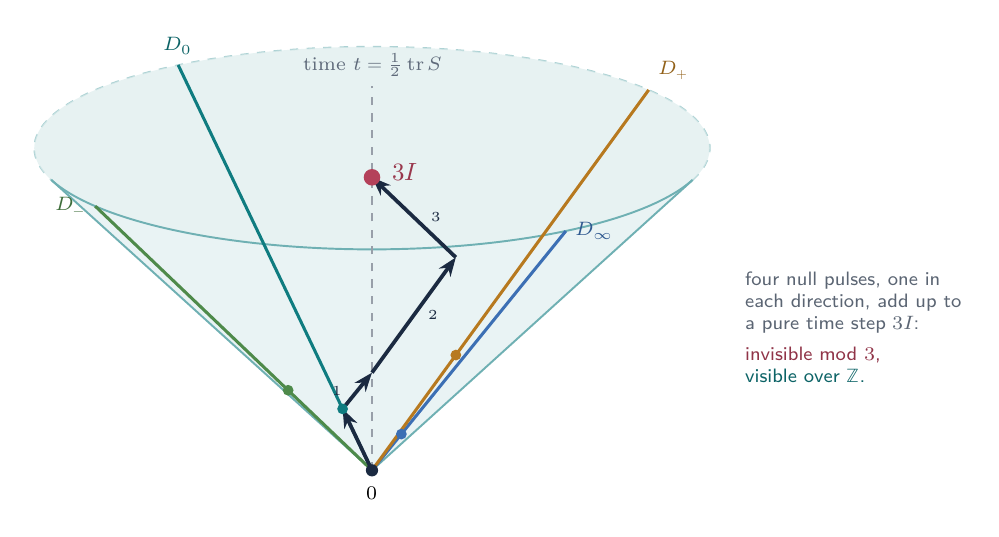
\begin{tikzpicture}[scale=1.3,>={Stealth[length=2.4mm]}]
  % generated by make_figures.py -- exact orthographic light cone
\coordinate (TL) at (-3.133,2.837);
\coordinate (TR) at (3.132,2.836);
\def\conecy{3.148}\def\conerx{3.300}\def\conery{0.990}
\def\conetl{198.32}\def\conetr{341.66}
\coordinate (RD0) at (-1.893,3.959);
\coordinate (PD0) at (-0.287,0.600);
\coordinate (RDinf) at (1.893,2.337);
\coordinate (PDinf) at (0.287,0.354);
\coordinate (RDp) at (2.703,3.716);
\coordinate (PDp) at (0.819,1.126);
\coordinate (RDm) at (-2.703,2.580);
\coordinate (PDm) at (-0.819,0.782);
\coordinate (Z0) at (0.000,0.000);
\coordinate (Z1) at (-0.287,0.600);
\coordinate (Z2) at (0.000,0.954);
\coordinate (Z3) at (0.819,2.080);
\coordinate (Z4) at (0.000,2.862);

  % back half of the rim (behind the cone)
  \draw[teal!35,line width=0.6pt,dashed] (0,\conecy) ++(\conetr:\conerx cm and \conery cm)
      arc[start angle=\conetr-360,end angle=\conetl,x radius=\conerx,y radius=\conery];
  % cone body
  \fill[teal!9] (0,0) -- (TL) arc[start angle=\conetl,end angle=\conetr,x radius=\conerx,y radius=\conery] -- cycle;
  \fill[teal!14,opacity=0.7] (0,\conecy) ellipse[x radius=\conerx,y radius=\conery];
  \draw[teal!60,line width=0.7pt] (0,0) -- (TL);
  \draw[teal!60,line width=0.7pt] (0,0) -- (TR);
  \draw[teal!60,line width=0.7pt] (TL) arc[start angle=\conetl,end angle=\conetr,x radius=\conerx,y radius=\conery];
  % time axis
  \draw[ink!45,dashed] (0,0) -- (0,3.75);
  \node[font=\scriptsize,text=ink!70,anchor=south] at (0,3.75) {time $t=\tfrac12\operatorname{tr}S$};
  % null rays
  \draw[teal,line width=1.1pt] (0,0) -- (RD0);
  \draw[sky,line width=1.1pt] (0,0) -- (RDinf);
  \draw[gold,line width=1.1pt] (0,0) -- (RDp);
  \draw[sage,line width=1.1pt] (0,0) -- (RDm);
  \node[font=\scriptsize,text=teal!80!black,anchor=south] at (RD0) {$D_0$};
  \node[font=\scriptsize,text=sky!80!black,anchor=west] at (RDinf) {$D_\infty$};
  \node[font=\scriptsize,text=gold!80!black,anchor=south west] at (RDp) {$D_+$};
  \node[font=\scriptsize,text=sage!80!black,anchor=east] at (RDm) {$D_-$};
  % zig-zag of four null pulses
  \draw[->,ink,line width=1.35pt] (Z0) -- (Z1);
  \draw[->,ink,line width=1.35pt] (Z1) -- (Z2);
  \draw[->,ink,line width=1.35pt] (Z2) -- (Z3);
  \draw[->,ink,line width=1.35pt] (Z3) -- (Z4);
  \foreach \k/\c in {D0/teal,Dinf/sky,Dp/gold,Dm/sage}{\fill[\c] (P\k) circle (1.5pt);}
  \fill[rose] (Z4) circle (2.3pt);
  \node[font=\small,text=rose!85!black,anchor=west] at ($(Z4)+(0.1,0.05)$) {$3I$};
  \node[font=\tiny,text=ink,anchor=east] at ($(Z1)!0.5!(Z2)+(-0.05,0)$) {$1$};
  \node[font=\tiny,text=ink,anchor=west] at ($(Z2)!0.5!(Z3)+(0.05,0)$) {$2$};
  \node[font=\tiny,text=ink,anchor=west] at ($(Z3)!0.5!(Z4)+(0.08,0)$) {$3$};
  \fill[ink] (0,0) circle (1.7pt);
  \node[font=\scriptsize,anchor=north] at (0,-0.06) {$0$};
  \node[font=\sffamily\scriptsize,text=slate,align=left,anchor=west] at (3.55,1.4)
    {four null pulses, one in\\each direction, add up to\\a pure time step $3I$:\\[3pt]
     \textcolor{rose!80!black}{invisible mod $3$,}\\\textcolor{teal!80!black}{visible over $\Z$.}};
\end{tikzpicture}
\caption{The real light cone of $2\times2$ symmetric matrices, drawn with time
$t=\tfrac12\tr S$ upward. The four null rays $D_0,D_\infty,D_\pm$ are the lifts of the
four points of the Bell line. The black zig-zag adds one pulse in each direction:
it ends on the time axis at $3I$. Modulo three this is the zero matrix --- the finite
present cannot see it --- but the integer lift records it as elapsed proper time.}
\label{fig:cone}
\end{figure}

\begin{physical}[What it means physically: two kinds of time]
Proposition~4.2 separates two notions that ordinary physics merges. The \emph{state} of
the finite present is a counter of null pulses modulo their common mode: $27$ values. But
a history that fires one pulse in every direction returns to the same present while
advancing by a pure time step upstairs. The finite chart measures \emph{where} you are;
the lifted history measures \emph{how long} it took. This is the structural shape of the
Page--Wootters idea that time is a relation between a clock and a system, and of the
distinction, in relativity, between coordinate position and proper time along a world
line. \tierB
\end{physical}

\subsection{Light-like steps: the null graph and its clock}

Join two of the $27$ events when they are null-separated. The resulting graph is
$8$-regular with $108$ edges, and it can be diagonalised exactly.

\begin{result}{Theorem 4.3 (spectral clock) \hfill \tierC}
The null graph has adjacency spectrum $8^{1}\,2^{12}\,(-1)^{8}\,(-4)^{6}$ and Laplacian
spectrum $0^{1}\,6^{12}\,9^{8}\,12^{6}$. At $t^\star=2\pi/9$ the continuous-time walk
$U=e^{-it^\star L}$ satisfies $U^3=I$, with eigenvalue multiplicities
$1^{9},\;\omega^{12},\;(\omega^2)^{6}$. The nine fixed modes are the constant mode and
the eight nonzero dual-null vectors of $\F_3^3$.
\cert{w33\_20260924\_null\_history\_spectral\_clock.py}
\end{result}

\begin{figure}[htbp]
\centering
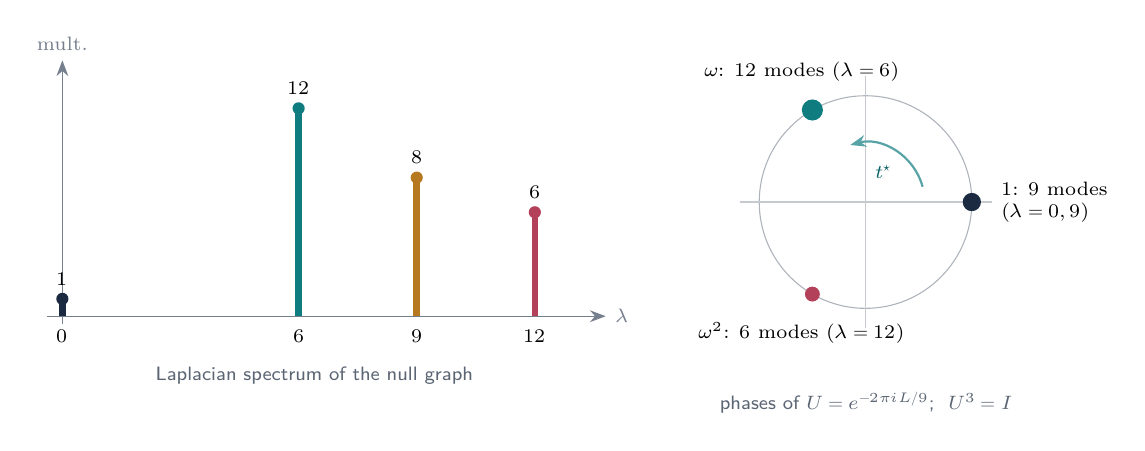
\begin{tikzpicture}[>={Stealth[length=2mm]}]
  % Laplacian spectrum stem plot
  \begin{scope}
    \draw[->,ink!60] (-0.2,0) -- (6.9,0) node[right,font=\scriptsize]{$\lambda$};
    \draw[->,ink!60] (0,-0.1) -- (0,3.25) node[above,font=\scriptsize]{mult.};
    \foreach \l/\m/\c in {0/1/ink,6/12/teal,9/8/gold,12/6/rose}{
      \pgfmathsetmacro{\xx}{\l*0.5}
      \pgfmathsetmacro{\yy}{\m*0.22}
      \draw[\c,line width=2.4pt] (\xx,0) -- (\xx,\yy);
      \fill[\c] (\xx,\yy) circle (2.2pt);
      \node[font=\scriptsize,anchor=south] at (\xx,\yy+0.05) {$\m$};
      \node[font=\scriptsize,anchor=north] at (\xx,-0.05) {$\l$};}
    \node[font=\sffamily\scriptsize,text=slate] at (3.2,-0.75) {Laplacian spectrum of the null graph};
  \end{scope}
  % phase circle
  \begin{scope}[xshift=10.2cm,yshift=1.45cm]
    \draw[ink!35] (0,0) circle (1.35);
    \draw[ink!25] (-1.6,0) -- (1.6,0); \draw[ink!25] (0,-1.6) -- (0,1.6);
    \fill[ink] (0:1.35) circle ({sqrt(9)*1.1pt});
    \fill[teal] (120:1.35) circle ({sqrt(12)*1.1pt});
    \fill[rose] (240:1.35) circle ({sqrt(6)*1.1pt});
    \node[font=\scriptsize,anchor=west,align=left] at (0:1.6) {$1$: $9$ modes\\($\lambda=0,9$)};
    \node[font=\scriptsize,anchor=south,align=center] at (120:1.62) {$\omega$: $12$ modes ($\lambda=6$)};
    \node[font=\scriptsize,anchor=north,align=center] at (240:1.62) {$\omega^2$: $6$ modes ($\lambda=12$)};
    \draw[->,teal!70,line width=0.8pt] (15:0.75) arc[start angle=15,end angle=105,radius=0.75];
    \node[font=\scriptsize,text=teal!80!black] at (60:0.45) {$t^\star$};
    \node[font=\sffamily\scriptsize,text=slate] at (0,-2.55) {phases of $U=e^{-2\pi iL/9}$; \ $U^3=I$};
  \end{scope}
\end{tikzpicture}
\caption{Left: the four Laplacian frequencies of the null graph. Right: running the
graph as a quantum walk for time $2\pi/9$ sends every mode to a cube root of unity ---
the $27$-event present carries an exact qutrit-valued clock.}
\label{fig:specclock}
\end{figure}

\begin{boundary}[A tempting identification that fails]
The nine fixed modes invite the reading ``$9=$ the nine operator histories of one qutrit''
from Section~3. It is false. The symmetry group acting on the fixed nine is faithful of
order $648$, whereas the projective qutrit Clifford group has order $216$, and the natural
Bell-line $S_4$ splits the eight null modes $4+4$ while $SL(2,3)$ is transitive on the
eight nonidentity qutrit Pauli labels. The count matches; the module does not.
\tierX\ (as an identification)
\end{boundary}

\subsection{History is a path, and paths do not close}

The null graph is connected with $27$ vertices and $108$ edges, so its cycle space has
rank $108-27+1=82$. Its fundamental group is the free group $F_{82}$ and its universal
cover is the infinite $8$-regular tree.

\begin{figure}[htbp]
\centering
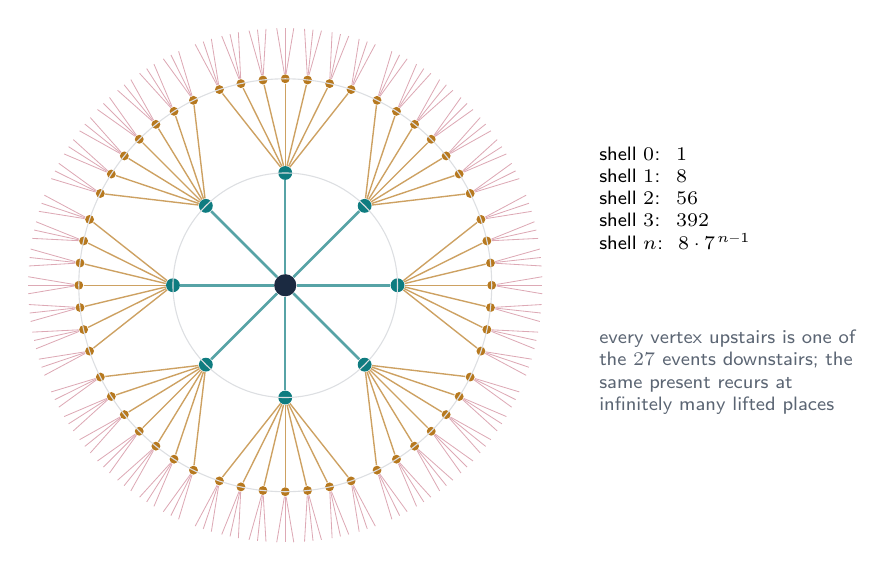
\begin{tikzpicture}[scale=0.92,
   nd/.style={circle,fill=#1,inner sep=0pt,minimum size=5pt}]
  \node[nd=ink,minimum size=8pt] (r) at (0,0) {};
  \foreach \k in {0,...,7}{
     \pgfmathsetmacro{\a}{90+45*\k}
     \node[nd=teal] (c\k) at (\a:1.55) {};
     \draw[teal!70,line width=0.9pt] (r) -- (c\k);
     \foreach \j in {0,...,6}{
        \pgfmathsetmacro{\b}{\a+ (\j-3)*6.2}
        \node[nd=gold,minimum size=3.2pt] (g\k\j) at (\b:2.85) {};
        \draw[gold!70,line width=0.5pt] (c\k) -- (g\k\j);
        \foreach \m in {-1,0,1}{
          \pgfmathsetmacro{\cc}{\b+\m*1.9}
          \draw[rose!45,line width=0.3pt] (g\k\j) -- (\cc:3.55);}
     }
  }
  \draw[ink!15] (0,0) circle (1.55); \draw[ink!15] (0,0) circle (2.85);
  \node[font=\sffamily\scriptsize,anchor=west,align=left] at (4.2,1.2)
   {shell $0$: \ $1$\\ shell $1$: \ $8$\\ shell $2$: \ $56$\\ shell $3$: \ $392$\\
    shell $n$: \ $8\cdot7^{\,n-1}$};
  \node[font=\sffamily\scriptsize,anchor=west,align=left,text=slate] at (4.2,-1.2)
   {every vertex upstairs is one of\\the $27$ events downstairs; the\\same present recurs at\\infinitely many lifted places};
\end{tikzpicture}
\caption{The universal cover of the null graph (only three grandchildren of each vertex
are drawn in the outer shell). The present is finite; the history is an unbounded tree.}
\label{fig:tree}
\end{figure}

\begin{result}{Theorem 4.4 (orientation and homology) \hfill \tierC}
\begin{enumerate}[label=(\roman*),leftmargin=1.5em]
\item The $108$ null edges are partitioned into $36$ edge-disjoint triangles, one for
      each point of $\W$ off the Bell line.
\item A signed sum of the $36$ triangle boundaries is a primitive cycle through all $108$
      edges with coefficients $\pm1$. The index-$2$ subgroup of the Bell stabiliser
      (order $648$) fixes it, and the other coset negates it: the cycle space splits
      objectwise as $82=1_{\text{orientation}}+81$.
\item Filling the $36$ triangles leaves first Betti number $46$, and the reduced
      $81$-dimensional module splits as $35+46$. The $46$ injects, by an explicit chain
      map, into $H_1(\W)$, which is itself $81$-dimensional and irreducible --- the
      Steinberg module of $\PSp(4,3)$.
\end{enumerate}
\cert{w33\_20260924\_history\_invariant\_cycle\_orientation.py}, \cert{w33\_20260924\_history\_to\_global\_h1\_intertwiner.py}
\end{result}

So there is exactly one global orientation of the history graph, and the symmetry group
of the ``now'' either preserves it or reverses it. This is a \emph{direction} for time,
but not yet an \emph{arrow}: reversing it is a symmetry of the geometry.

\begin{center}
\small
\renewcommand{\arraystretch}{1.25}
\begin{tabularx}{\textwidth}{@{}>{\raggedright\arraybackslash}p{3.5cm}X>{\raggedright\arraybackslash}p{3.3cm}@{}}
\toprule
\textbf{Temporal observable} & \textbf{Lives on} & \textbf{Reversible?}\\
\midrule
position in the present & one of $27$ events & yes\\
step count & length of a path in the null graph & yes\\
reduced word & element of the free group $F_{82}$ & yes\\
winding & homology class in $\Z^{82}$; the common mode of Prop.~4.2 & yes\\
orientation & the sign of the unique invariant cycle & yes (up to a symmetry)\\
coherent phase & the Weil phase $\mu_{12}$ below & yes (complex conjugation)\\
records & classical outcomes kept by an observer & \textbf{no}: discarding them is the arrow\\
\bottomrule
\end{tabularx}
\end{center}

\subsection{A coherent twist: the twelfth roots of unity}

For the qutrit Fourier transform $F$ and the chirp $G=\mathrm{diag}(1,\omega,\omega)$ one
has $(FG)^3=i\,F^2$. The metaplectic (Weil) representation that implements the symplectic
symmetries on quantum states therefore carries phases in $\langle i,\omega\rangle=\mu_{12}$.
Across the $27$ quadratic forms of the present, the Weil phases occur with census
$1^{13},\;i^{4},\;(-1)^{6},\;(-i)^{4}$. Complex conjugation --- the quantum-mechanical time
reversal --- sends $i\mapsto -i$ and $\omega\mapsto\omega^{-1}$. This is a reversible,
coherent orientation mechanism, distinct from entropy production. \tierC\
(\cert{w33\_20260924\_temporal\_maslov\_mu12.py})

\subsection{Four clocks: the Hesse striations and the tetracode}

The four points of the Bell line --- the four null directions --- reappear in a second,
seemingly unrelated place. Identify the nine operator histories $\ket{i}\!\bra{j}$ with the
nine points of the affine plane $AG(2,3)=\F_3^2$. Its $12$ lines fall into four
\emph{parallel classes} of three lines each, one class for each direction
$v\in\mathbb{P}^1(\F_3)$. Each class is a way of reading the nine cells as ``three ticks of
a clock''; we call the four classes the four \emph{Hesse clocks}.

\begin{figure}[htbp]
\centering
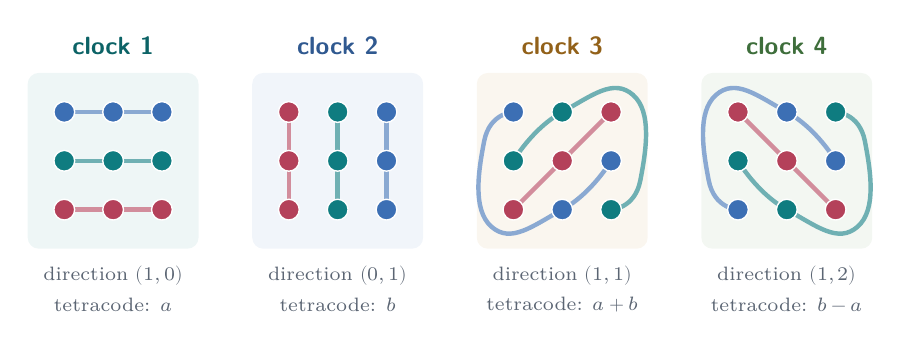
\begin{tikzpicture}[scale=0.62,
    dot/.style={circle,fill=#1,draw=white,line width=0.5pt,inner sep=0pt,minimum size=7.5pt}]
  \def\panel#1#2#3#4#5{% xshift, title color, title, ray, tetracode
    \begin{scope}[xshift=#1 cm]
      \fill[#2!7,rounded corners=4pt] (-0.75,-0.8) rectangle (2.75,2.8);
      \node[font=\sffamily\small\bfseries,text=#2!80!black] at (1,3.35) {#3};
      \node[font=\scriptsize,text=slate] at (1,-1.35) {direction $#4$};
      \node[font=\scriptsize,text=slate] at (1,-1.95) {tetracode: $#5$};
    \end{scope}}
  \panel{0}{teal}{clock 1}{(1,0)}{a}
  \panel{4.6}{sky}{clock 2}{(0,1)}{b}
  \panel{9.2}{gold}{clock 3}{(1,1)}{a+b}
  \panel{13.8}{sage}{clock 4}{(1,2)}{b-a}
  % clock 1: horizontal lines y=const
  \begin{scope}[xshift=0cm]
    \foreach \y/\c in {0/rose,1/teal,2/sky}{\draw[\c!60,line width=1.6pt] (0,\y) -- (2,\y);
      \foreach \x in {0,1,2}{\node[dot=\c] at (\x,\y) {};}}
  \end{scope}
  % clock 2: vertical lines
  \begin{scope}[xshift=4.6cm]
    \foreach \x/\c in {0/rose,1/teal,2/sky}{\draw[\c!60,line width=1.6pt] (\x,0) -- (\x,2);
      \foreach \y in {0,1,2}{\node[dot=\c] at (\x,\y) {};}}
  \end{scope}
  % clock 3: y - x = const (slope 1): {(0,0),(1,1),(2,2)}, {(0,1),(1,2),(2,0)}, {(0,2),(1,0),(2,1)}
  \begin{scope}[xshift=9.2cm]
    \draw[rose!60,line width=1.6pt] (0,0) -- (2,2);
    \draw[teal!60,line width=1.6pt] plot[smooth,tension=0.9] coordinates {(0,1) (1,2) (2.45,2.35) (2.6,0.6) (2,0)};
    \draw[sky!60,line width=1.6pt] plot[smooth,tension=0.9] coordinates {(2,1) (1,0) (-0.45,-0.35) (-0.6,1.4) (0,2)};
    \foreach \p in {(0,0),(1,1),(2,2)}{\node[dot=rose] at \p {};}
    \foreach \p in {(0,1),(1,2),(2,0)}{\node[dot=teal] at \p {};}
    \foreach \p in {(0,2),(1,0),(2,1)}{\node[dot=sky] at \p {};}
  \end{scope}
  % clock 4: y + x = const (slope 2): {(0,0),(1,2),(2,1)}, {(0,1),(1,0),(2,2)}, {(0,2),(1,1),(2,0)}
  \begin{scope}[xshift=13.8cm]
    \draw[rose!60,line width=1.6pt] (0,2) -- (2,0);
    \draw[teal!60,line width=1.6pt] plot[smooth,tension=0.9] coordinates {(0,1) (1,0) (2.45,-0.35) (2.6,1.4) (2,2)};
    \draw[sky!60,line width=1.6pt] plot[smooth,tension=0.9] coordinates {(2,1) (1,2) (-0.45,2.35) (-0.6,0.6) (0,0)};
    \foreach \p in {(0,2),(1,1),(2,0)}{\node[dot=rose] at \p {};}
    \foreach \p in {(0,1),(1,0),(2,2)}{\node[dot=teal] at \p {};}
    \foreach \p in {(0,0),(1,2),(2,1)}{\node[dot=sky] at \p {};}
  \end{scope}
\end{tikzpicture}
\caption{The four Hesse clocks. Each panel shows the nine operator histories of one
qutrit as the affine plane $\F_3^2$, split into three parallel lines (the three ``ticks'').
Lines of the two diagonal classes wrap around, as on a torus. The four panels are labelled
by the four points of $\mathbb{P}^1(\F_3)$ --- the same four labels as the null
directions of Figure~\ref{fig:bellview} --- and by the coordinate of the tetracode they
read.}
\label{fig:hesse}
\end{figure}

\begin{result}{Theorem 4.5 (one $S_4$ for three structures) \hfill \tierC}
The four projective null directions of the present, the four Hesse clocks, and (Section~5)
four orthogonal $A_2$ root systems inside $E_8$ are all indexed by
$\mathbb{P}^1(\F_3)=\{(1,0),(0,1),(1,1),(1,2)\}$. For every one of the $24$ elements of
$PGL(2,3)\cong S_4$, the induced permutations of the three four-element sets are
identical. The larger groups differ (the Bell stabiliser acts with kernel $27$, $AGL(2,3)$
with kernel $18$); the common object is the quotient $S_4$ and its action.
\cert{w33\_20260924\_null\_hesse\_4a2\_s4\_intertwiner.py}
\end{result}

The four clocks also carry a code. Evaluate the linear ``clock reading''
$\ell_{(a,b)}(x,y)=ax+by$ at oriented representatives $(1,0),(0,1),(1,1),(2,1)$ of the four
directions. The result is
\[
(a,\;b,\;a+b,\;b-a)\in\F_3^4 ,
\]
and the nine such words are \emph{exactly} the repository's frozen \emph{tetracode}, the
$[4,2,3]_3$ code at the heart of the ternary Golay code and of the $E_8$ lattice's
tetracode construction --- no coordinate permutation needed. \tierC\
(\cert{w33\_pass10946\_clock\_code\_cone\_objectwise.py})

\begin{figure}[htbp]
\centering
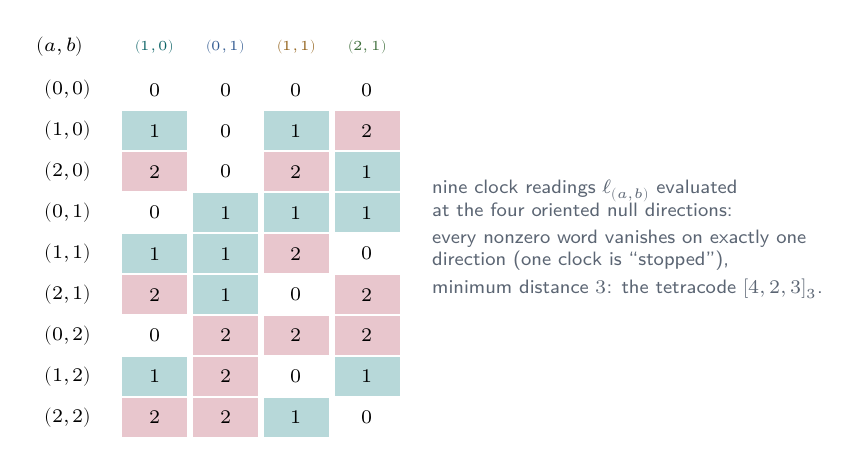
\begin{tikzpicture}[cell/.style={minimum width=8.6mm,minimum height=5.2mm,draw=white,line width=0.8pt,font=\scriptsize}]
  \def\cc#1{\ifcase#1 white\or teal!30\or rose!30\fi}
  \node[font=\sffamily\scriptsize\bfseries] at (-1.2,0.55) {$(a,b)$};
  \foreach \j/\t/\c in {0/{(1,0)}/teal,1/{(0,1)}/sky,2/{(1,1)}/gold,3/{(2,1)}/sage}{
     \node[font=\tiny,text=\c!80!black] at (\j*0.9,0.55) {$\t$};}
  \foreach \a/\b [count=\r from 0] in {0/0,1/0,2/0,0/1,1/1,2/1,0/2,1/2,2/2}{
     \pgfmathtruncatemacro{\w}{\a}
     \pgfmathtruncatemacro{\x}{\b}
     \pgfmathtruncatemacro{\y}{mod(\a+\b,3)}
     \pgfmathtruncatemacro{\z}{mod(\b-\a+3,3)}
     \node[font=\scriptsize] at (-1.1,-\r*0.52) {$(\a,\b)$};
     \foreach \v [count=\j from 0] in {\w,\x,\y,\z}{
        \node[cell,fill=\cc{\v}] at (\j*0.9,-\r*0.52) {$\v$};}
  }
  \node[font=\sffamily\scriptsize,text=slate,align=left,anchor=west] at (3.4,-1.9)
   {nine clock readings $\ell_{(a,b)}$ evaluated\\at the four oriented null directions:\\[2pt]
    every nonzero word vanishes on exactly one\\direction (one clock is ``stopped''),\\[2pt]
    minimum distance $3$: the tetracode $[4,2,3]_3$.};
\end{tikzpicture}
\caption{The tetracode as a table of clock readings (colour: $1$ teal, $2$ rose).}
\label{fig:tetracode}
\end{figure}

\begin{physical}[What it means physically: a frame and an orientation]
A projective direction picks a clock \emph{frame}: which three-way split of the nine
histories counts as the ticks. Choosing a representative of the direction --- $(1,2)$ or
its negative $(2,1)$ --- picks an \emph{orientation} of that clock. The tetracode's
peculiar sign $b-a$ (rather than $a-b$) in its last coordinate is exactly this orientation
choice. Each nonzero codeword stops exactly one of the four clocks; $4$ stopped clocks
$\times$ $2$ orientations $\times$ $3$ origins give $24$ complete clock calibrations.
\end{physical}

The other research track found a further layer (Pass~10948, which we cite rather than
re-derive). Over $\F_3$, $x^4+1=(x^2+x-1)(x^2-x-1)$, and after flipping the orientation of
one clock the tetracode becomes the ideal $(x^2\pm x-1)$ in $\F_3[x]/(x^4+1)$: the cyclic
shift of clock readings with a sign, $N(c_0,c_1,c_2,c_3)=(-c_3,c_0,c_1,c_2)$, preserves it
and satisfies $N^4=-I$, $N^8=I$. The two orientations give two transverse self-dual
tetracodes forming a hyperbolic pair; the negacyclic presentation of the tetracode was used
in a cyclotomic $E_8$ construction by Watanabe \emph{et al.} \cite{WBCV2018}. \tierC\
(\cert{w33\_pass10948\_clock\_tetracode\_negacyclic\_hyperbolic\_bridge.py}) A clock whose
fourth tick is a sign flip and whose eighth tick is the identity is the finite shadow of
something we meet again in Section~8: a rotation by $2\pi$ that acts as $-1$ on spinors.

\subsection{Clocks as relations: the Page--Wootters weld}

Label a clock qutrit's phase by $c\in\F_3$ and a system's phase by $p\in\F_3$. The four
directions of $\F_3^2$ are $c$, $p$, $c+p$ and $c-p$. For an order-three evolution $U$ of
the system, the two stationary ``history states''
\[
(X_{\text{clock}}\otimes U)\ket{\Psi_+}=\ket{\Psi_+},\qquad
(X_{\text{clock}}\otimes U^{-1})\ket{\Psi_-}=\ket{\Psi_-}
\]
are supported, in the clock's phase basis, exactly on $c+p=0$ and $c-p=0$: the two
correlated directions. The two remaining directions ($c=0$, $p=0$) are the uncorrelated
axes. On the committed $E_8$ basis, pairs of axis-only backgrounds generate a subalgebra of
dimension $24$, whereas any graph-correlated background generates all $248$
dimensions. \tierC\ (\cert{w33\_20260924\_page\_wootters\_diagonal\_weld.py})

\begin{plainwords}
In 1983 Don Page and William Wootters proposed \cite{PageWootters} that the universe as a whole might be
static, with time emerging as a correlation between a ``clock'' part and the rest. The
finite version above is exact: a state that is globally unchanging, yet in which the
clock reading and the system's phase are locked together. Only the two
\emph{correlated} clock directions produce such states --- and only they, in the $E_8$
computation, generate the whole algebra.
\end{plainwords}

\subsection{A second light cone: Hermitian $3+1$, and a weld that fails}

Replace real symmetric matrices by Hermitian ones over $\F_9=\F_3(u)$, $u^2=-1$:
$X=\begin{psmallmatrix} a&z\\ \bar z&c\end{psmallmatrix}$ with $z=x+uy$. Then
$\det X=ac-x^2-y^2$ is a form in four variables --- a $3+1$-dimensional finite Minkowski
space.

\begin{result}{Theorem 4.6 (the Hermitian present is a spread) \hfill \tierC}
The $81$ Hermitian events split $21+30+30$ by determinant, and the $40$ projective
directions split $10+15+15$. An explicit map sends the Hermitian quadric to the elliptic
hyperplane section of $Q(4,3)$, and under the line dictionary the ten null directions
become ten pairwise disjoint lines of $\W$ covering all $40$ points --- a \emph{spread}.
The $36$ elliptic sections are exactly the $36$ spreads of $\W$.
\cert{w33\_20260924\_hermitian\_3p1\_spread\_bridge.py}
\end{result}

\begin{figure}[htbp]
\centering
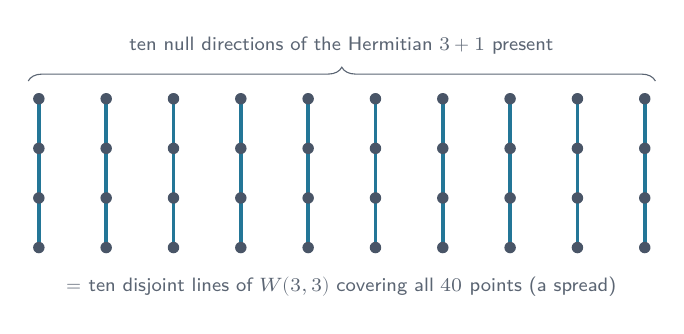
\begin{tikzpicture}[scale=0.9]
  \foreach \k in {0,...,9}{
    \pgfmathsetmacro{\hue}{\k*10}
    \draw[teal!55!sky,line width=1.3pt,rounded corners=2pt] (\k*0.95,0) -- (\k*0.95,2.1);
    \foreach \j in {0,...,3}{\fill[ink!80] (\k*0.95,\j*0.7) circle (2.3pt);}}
  \draw[decorate,decoration={brace,amplitude=5pt},slate] (-0.15,2.35) -- (8.7,2.35);
  \node[font=\sffamily\scriptsize,text=slate] at (4.27,2.85) {ten null directions of the Hermitian $3+1$ present};
  \node[font=\sffamily\scriptsize,text=slate] at (4.27,-0.55) {$=$ ten disjoint lines of $\W$ covering all $40$ points (a spread)};
\end{tikzpicture}
\caption{The Hermitian $3+1$ light cone is a partition of the forty points into ten
complete measurement contexts --- a complete ``schedule'' for measuring every
two-qutrit direction exactly once.}
\label{fig:spread}
\end{figure}

\begin{boundary}[The complex-structure weld does not exist]
One might hope to weld the Hermitian light cone to the symplectic geometry through a
single complex structure $J$ ($J^2=-I$) with $\Omega(x,y)=B(Jx,y)$. Exhausting all
$729$ candidates finds none. The light cone and the qutrit geometry meet through the
point/line duality of Section~2, not through one compatible $J$. \tierX\ (for the direct weld)
\end{boundary}

\subsection{The arrow: forgetting two trits}

Every structure so far is reversible. Where does irreversibility come from? There is a
sharp answer.

\begin{result}{Theorem 4.7 (the price of an arrow) \hfill \tierT}
For every qutrit state $\rho$,
\[
\frac19\sum_{u\in\F_3^2} P_u\,\rho\,P_u^\dagger \;=\; \tr(\rho)\,\frac{I}{3}.
\]
Each map $\rho\mapsto P_u\rho P_u^\dagger$ is unitary and reversible; their average,
obtained by forgetting which $u$ occurred, is the completely depolarising channel, which
erases every state to the same fixed point. The forgotten record is two trits, so by
Landauer's principle \cite{Landauer} making a qutrit clock irreversible in this way dissipates at least
$2\,k_BT\ln3$ per step.
\end{result}

\begin{proof}
The left side, as a function of $\rho$, commutes with conjugation by every $P_v$ (which
merely permutes the $u$'s up to phases that cancel). Its image $\Sigma$ therefore
commutes with all nine Paulis, which span $\End(\C^3)$, so $\Sigma$ is a scalar; taking
traces gives the scalar $\tr(\rho)/3$.
\end{proof}

\begin{physical}[What it means physically]
The finite present has a light cone; the history has an orientation; the Weil phase has a
handedness. None of these is an arrow of time, because each can be reversed by a symmetry.
The arrow appears exactly when a record is discarded. For a qutrit clock the minimal
record is the two-trit label of the Pauli step --- the photonic papers' ``two trits per
cycle'' (\cert{bt823\_the\_closure.py}; see also \cert{w33\_20260924\_adqc\_record\_arrow.py}) --- and discarding it turns a reversible tick into the maximally
irreversible channel. This is the finite form of the modern view that the thermodynamic
arrow is information loss, and it is \emph{consistent} with the Connes--Rovelli idea of
Section~3: a state can orient time, but only forgetting makes it flow one way. \tierB
\end{physical}

\begin{keyidea}
Three layers of time, exactly separated: a finite present with a light cone ($27$
events, $t^2-x^2-y^2$); an unbounded, oriented history (a free group, an $8$-regular tree,
a winding the present cannot see); and an arrow that costs exactly two trits of forgotten
record per tick.
\end{keyidea}

\begin{boundary}
None of this derives a continuum space-time, a speed of light, a metric that curves, or
gravity. The light cone here is an algebraic form over a three-element field; ``null''
means ``shares a measurement''. Whether the present, history and arrow of the finite model
are the finite shadows of physical time is a bridge hypothesis, and the dynamics that would
make it testable --- a Hamiltonian, an energy scale --- is not supplied by the geometry.
\tierO
\end{boundary}

\section{\texorpdfstring{$E_8$}{E8} from nine histories}
\label{sec:e8}

$E_8$ is the largest of the five exceptional simple Lie algebras: $248$ dimensions, $240$
roots, a symmetry so rigid that it appears, often unexpectedly, in string theory, in the
densest packing of spheres in eight dimensions, and in the physics of certain magnetic
materials. This section shows that one qutrit's nine operator histories build $E_8$ in a
way in which every piece has a meaning in the finite geometry --- and it records
carefully one famous coincidence that turned out to be a trap.

\begin{plainwords}
A Lie algebra is the ``infinitesimal'' version of a continuous symmetry: the set of all
directions in which you can nudge a system while keeping its rules intact, together with
the rule (the \emph{bracket}) for what happens when two nudges are combined in opposite
orders. Its \emph{roots} are the special directions that the symmetry's own ``clock''
(its maximal commuting part) rotates at definite rates. $E_8$ has $240$ of them.
\end{plainwords}

\subsection{Eighty plus eighty-four plus eighty-four}

Recall from Section~3 that the $80$ non-identity two-sided Weyl maps on one qutrit span
$\sll_9$, the Lie algebra of traceless $9\times9$ matrices acting on the nine operator
histories $\ket{i}\!\bra{j}$. Now add \emph{packets}: unordered triples of histories. There
are $\binom93=84$ of them, forming the representation $\Lambda^3\C^9$; their duals form
$\Lambda^6\C^9$, another $84$. A classical construction \cite{Adams1996,Baez2002} makes
\[
E_8 \;=\; \sll_9\;\oplus\;\Lambda^3\C^9\;\oplus\;\Lambda^6\C^9,\qquad
248=80+84+84 ,
\]
into a Lie algebra. On the nine history cells the brackets are literal packet operations:
$E_{ij}$ replaces cell $j$ by cell $i$ inside a packet; two disjoint triples bracket to the
complementary six-set; a triple and a six-set differing by one cell contract to an
$E_{ij}$; opposite packets return a Cartan direction. \tierC\
(\cert{w33\_20260924\_temporal\_su9\_e8\_compiler.py},
\cert{w33\_20260924\_temporal\_a8\_e8\_process\_bracket.py})

\subsection{Hesse lines are copies of \texorpdfstring{$A_2$}{A2}}

Place the nine histories on the affine plane $\F_3^2$ as in Figure~\ref{fig:hesse}. A
triple $S$ of cells labels the root
\[
w_S=\sum_{i\in S}e_i-\tfrac13\sum_{i=1}^9e_i ,\qquad w_S\cdot w_T=|S\cap T|-1 .
\]
(Indeed $|w_S|^2=3-2+1=2$.) The $84$ triples fall into two orbits of the affine group
$AGL(2,3)$ (order $432$): the $12$ \emph{lines} of the plane and the $72$ non-collinear
\emph{triangles}.

\begin{result}{Theorem 5.1 (four clocks, four $A_2$'s) \hfill \tierT\ \tierC}
The three lines of one parallel class give three roots with pairwise products $-1$ and
sum $0$; with their negatives they form a root system $A_2$. Lines of different classes
meet in exactly one cell, so their roots are orthogonal. The $12$ Hesse lines therefore
span a reflection-closed subsystem $4A_2\subset E_8$, one $A_2$ per clock, and the root
shell refines as
\[
240\;=\;\underbrace{72}_{A_8}\;+\;\underbrace{24}_{\text{Hesse }4A_2}\;+\;\underbrace{144}_{\text{triangles}} .
\]
\cert{w33\_20260924\_temporal\_hesse\_4a2\_a8\_bridge.py}
\end{result}

\begin{proof}
Disjoint triples have $|S\cap T|=0$, hence product $-1$; the three lines of a class
partition the nine cells, so $\sum w_S=\sum_i e_i-3\cdot\frac13\sum_ie_i=0$. Two
non-parallel lines of an affine plane meet in one point, giving product $1-1=0$.
\end{proof}

\begin{figure}[htbp]
\centering
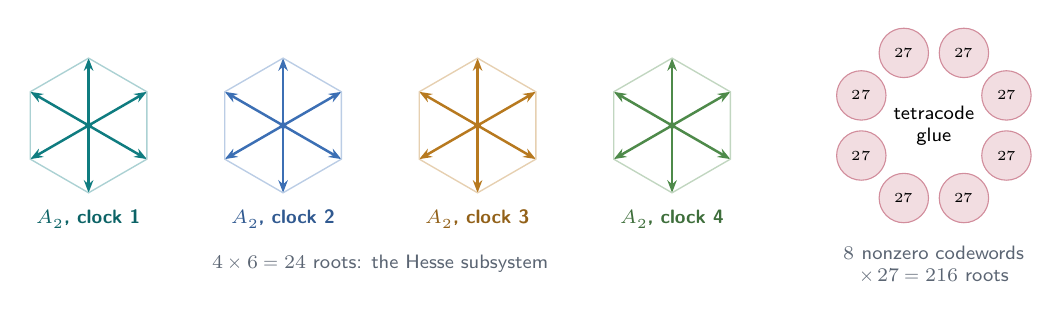
\begin{tikzpicture}[scale=0.95]
  % four A2 hexagons, one per clock
  \foreach \c/\n/\x in {teal/1/0,sky/2/2.6,gold/3/5.2,sage/4/7.8}{
    \begin{scope}[xshift=\x cm]
      \foreach \k in {0,...,5}{
        \draw[\c,line width=0.9pt,-{Stealth[length=1.6mm]}] (0,0) -- (60*\k+30:0.9);}
      \draw[\c!35,line width=0.5pt] (30:0.9) \foreach \k in {1,...,5}{ -- (60*\k+30:0.9)} -- cycle;
      \fill[\c] (0,0) circle (1.3pt);
      \node[font=\sffamily\scriptsize\bfseries,text=\c!80!black] at (0,-1.25) {$A_2$, clock \n};
    \end{scope}}
  \node[font=\sffamily\scriptsize,text=slate] at (3.9,-1.85) {$4\times 6=24$ roots: the Hesse subsystem};
  % glue sectors
  \begin{scope}[xshift=11.3cm,yshift=0cm]
    \foreach \k in {0,...,7}{
      \pgfmathsetmacro{\a}{\k*45+22.5}
      \fill[rose!18,draw=rose!60] (\a:1.05) circle (0.33);
      \node[font=\tiny] at (\a:1.05) {$27$};}
    \node[font=\sffamily\scriptsize,align=center] at (0,0) {tetracode\\glue};
    \node[font=\sffamily\scriptsize,text=slate,align=center] at (0,-1.85) {$8$ nonzero codewords\\$\times\,27=216$ roots};
  \end{scope}
\end{tikzpicture}
\caption{$E_8$ assembled from four clocks. Each Hesse clock contributes one $A_2$ root
system (left). The remaining $216$ roots come in eight sectors of $27$, one for each
nonzero word of the tetracode (right): $240=4\cdot6+8\cdot27$.}
\label{fig:a24}
\end{figure}

\subsection{The glue is the tetracode, and the tetracode is the clock}

The lattice $E_8$ contains the sublattice $A_2^4$ with quotient $\F_3^2$, and the
well-known construction of $E_8$ from the tetracode \cite{ConwaySloane} reads it as
\[
E_8=\bigcup_{c\in\mathcal{T}}\bigl(c+A_2^{\,4}\bigr),\qquad
240=4\cdot6+8\cdot27 ,
\]
where $\mathcal{T}\subset\F_3^4$ is the tetracode: each of the eight nonzero codewords has
weight three, and contributes $3^3=27$ minimal vectors. Combined with Section~4, the
four glue coordinates are the four clocks and the eight nonzero sectors are the eight
oriented, nonzero linear clock readings. \tierT\ (classical) \ \tierC\ (the clock reading,
\cert{w33\_pass10946\_clock\_code\_cone\_objectwise.py})

\subsection{A trap: \texorpdfstring{$240=240$}{240 = 240}}
\label{sec:e8-trap}

The collinearity graph of $\W$ has $240$ edges, and $E_8$ has $240$ roots. For years the
repository looked for a natural bijection between them. The question has a precise and
negative answer.

\begin{result}{Theorem 5.2 (no equivariant bijection) \hfill \tierC}
The two groups of order $51\,840$ of Section~2 each do only half the job:
\begin{itemize}
\item $\PGSp(4,3)\cong W(E_6)$ acts faithfully and transitively on the $240$ edges of $\W$,
      but \emph{intransitively} on the $240$ roots of $E_8$;
\item $\Sp(4,3)$ acts faithfully and transitively on the $240$ roots, but its centre acts
      trivially on the edges, so its edge action is not faithful.
\end{itemize}
Hence no bijection between edges and roots is equivariant for a common group.
\cert{w33\_pass1020\_e8\_transitive\_51840.g}
\end{result}

What \emph{does} exist is better. The Weyl group of $E_8$ contains a regular element $w$
of order three. By Springer's theory \cite{Springer} its centraliser is the complex reflection group
$G_{32}\cong\Z_3\times\Sp(4,3)$ of order $155\,520$ --- the symmetry group of the
\emph{Witting polytope}, whose $240$ vertices in $\C^4$ are the $E_8$ roots.

\begin{result}{Theorem 5.3 (the $6:1$ fibration) \hfill \tierC}
The $240$ roots of $E_8$ fall into $40$ complex lines $\{\pm v,\pm\omega v,\pm\omega^2 v\}$,
each a copy of the six Eisenstein units. $\Sp(4,3)$ permutes the $40$ lines with
subdegrees $1,12,27$: the quotient is the collinearity graph of $\W$ --- on its
\emph{points}, not its lines. The fibre group is $\langle c^5\rangle\cong\Z_6$ for a
Coxeter element $c$ of $W(E_8)$.
\cert{w33\_pass1021\_e8\_fibration\_over\_forty.g}
\end{result}

\begin{figure}[htbp]
\centering
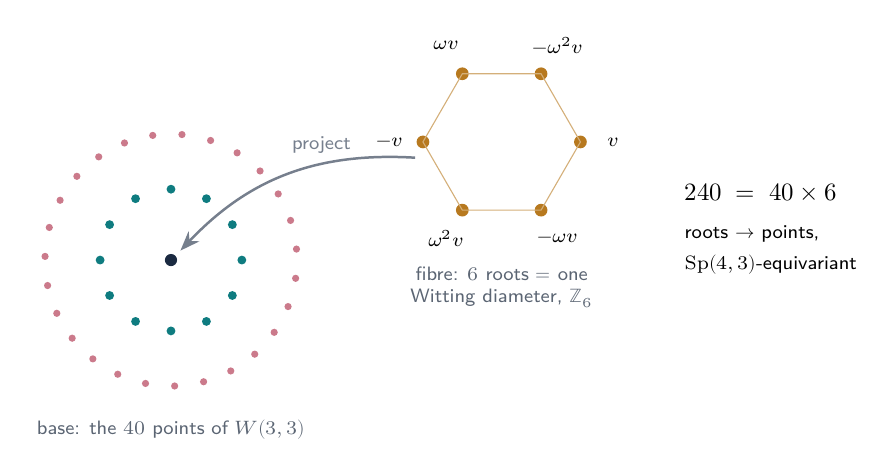
\begin{tikzpicture}[scale=1]
  % base: 40 points (sketch: the 1+12+27 view)
  \begin{scope}
    \fill[ink] (0,0) circle (2.2pt);
    \foreach \k in {0,...,11}{\fill[teal] ({30*\k}:0.9) circle (1.6pt);}
    \foreach \k in {0,...,26}{\fill[rose!70] ({360*\k/27+5}:1.6) circle (1.3pt);}
    \node[font=\sffamily\scriptsize,text=slate] at (0,-2.15) {base: the $40$ points of $\W$};
  \end{scope}
  % fibre over one point
  \draw[-{Stealth[length=2.5mm]},ink!60,line width=0.9pt] (3.1,1.3) to[bend right=25] node[above,font=\sffamily\scriptsize,pos=0.35]{project} (0.12,0.12);
  \begin{scope}[xshift=4.2cm,yshift=1.5cm]
    \foreach \k/\lab in {0/{v},1/{-\omega^2v},2/{\omega v},3/{-v},4/{\omega^2 v},5/{-\omega v}}{
      \fill[gold] (60*\k:1.0) circle (2.3pt);
      \node[font=\scriptsize] at (60*\k:1.42) {$\lab$};}
    \draw[gold!60] (0:1) \foreach \k in {1,...,5}{-- (60*\k:1)} -- cycle;
    \node[font=\sffamily\scriptsize,text=slate,align=center] at (0,-1.85) {fibre: $6$ roots $=$ one\\Witting diameter, $\Z_6$};
  \end{scope}
  \node[font=\sffamily\small,align=left,anchor=west] at (6.4,0.4)
   {$240\;=\;40\times6$\\[3pt]\scriptsize roots $\to$ points,\\\scriptsize $\Sp(4,3)$-equivariant};
\end{tikzpicture}
\caption{The correct relation between $E_8$ and $\W$: not edges to roots, but a
six-to-one map from roots to points, whose fibres are the Eisenstein unit hexagons.}
\label{fig:fibration}
\end{figure}

\begin{figure}[p]
\centering
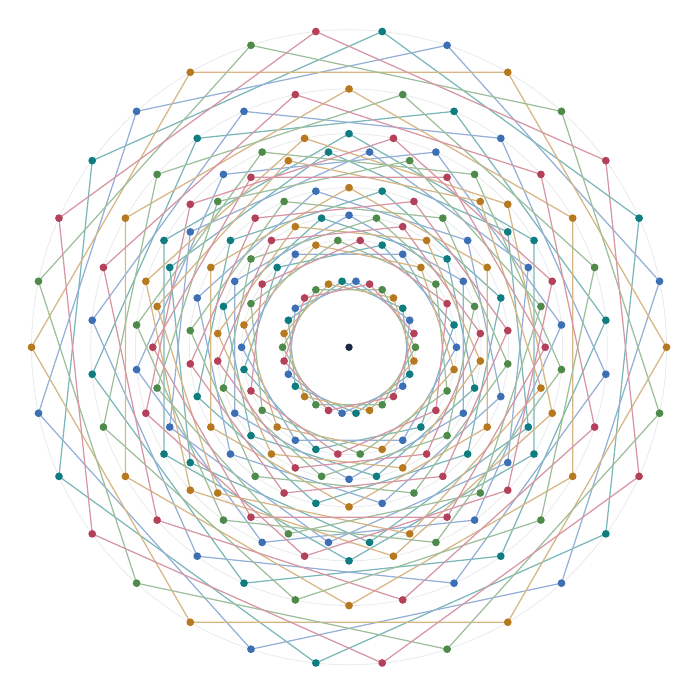
\begin{tikzpicture}[scale=1.12]
  % generated by make_figures.py -- E8 Coxeter plane, 40 hexagonal fibres
\draw[ink!10,line width=0.3pt] (0,0) circle (0.753);
\draw[ink!10,line width=0.3pt] (0,0) circle (1.218);
\draw[ink!10,line width=0.3pt] (0,0) circle (1.497);
\draw[ink!10,line width=0.3pt] (0,0) circle (1.810);
\draw[ink!10,line width=0.3pt] (0,0) circle (2.225);
\draw[ink!10,line width=0.3pt] (0,0) circle (2.422);
\draw[ink!10,line width=0.3pt] (0,0) circle (2.929);
\draw[ink!10,line width=0.3pt] (0,0) circle (3.600);
\draw[teal!55,line width=0.45pt] (-1.721,-0.559) -- (-0.376,-1.770) -- (1.345,-1.211) -- (1.721,0.559) -- (0.376,1.770) -- (-1.345,1.211) -- cycle;
\fill[teal] (-1.721,-0.559) circle (1.25pt);
\fill[teal] (-0.376,-1.770) circle (1.25pt);
\fill[teal] (1.345,-1.211) circle (1.25pt);
\fill[teal] (1.721,0.559) circle (1.25pt);
\fill[teal] (0.376,1.770) circle (1.25pt);
\fill[teal] (-1.345,1.211) circle (1.25pt);
\draw[teal!55,line width=0.45pt] (-1.191,-0.253) -- (-0.376,-1.158) -- (0.815,-0.905) -- (1.191,0.253) -- (0.376,1.158) -- (-0.815,0.905) -- cycle;
\fill[teal] (-1.191,-0.253) circle (1.25pt);
\fill[teal] (-0.376,-1.158) circle (1.25pt);
\fill[teal] (0.815,-0.905) circle (1.25pt);
\fill[teal] (1.191,0.253) circle (1.25pt);
\fill[teal] (0.376,1.158) circle (1.25pt);
\fill[teal] (-0.815,0.905) circle (1.25pt);
\draw[sky!55,line width=0.45pt] (-1.218,-0.000) -- (-0.609,-1.055) -- (0.609,-1.055) -- (1.218,0.000) -- (0.609,1.055) -- (-0.609,1.055) -- cycle;
\fill[sky] (-1.218,-0.000) circle (1.25pt);
\fill[sky] (-0.609,-1.055) circle (1.25pt);
\fill[sky] (0.609,-1.055) circle (1.25pt);
\fill[sky] (1.218,0.000) circle (1.25pt);
\fill[sky] (0.609,1.055) circle (1.25pt);
\fill[sky] (-0.609,1.055) circle (1.25pt);
\draw[teal!55,line width=0.45pt] (-0.609,-0.442) -- (0.079,-0.748) -- (0.688,-0.306) -- (0.609,0.442) -- (-0.079,0.748) -- (-0.688,0.306) -- cycle;
\fill[teal] (-0.609,-0.442) circle (1.25pt);
\fill[teal] (0.079,-0.748) circle (1.25pt);
\fill[teal] (0.688,-0.306) circle (1.25pt);
\fill[teal] (0.609,0.442) circle (1.25pt);
\fill[teal] (-0.079,0.748) circle (1.25pt);
\fill[teal] (-0.688,0.306) circle (1.25pt);
\draw[sky!55,line width=0.45pt] (-0.688,-0.306) -- (-0.079,-0.748) -- (0.609,-0.442) -- (0.688,0.306) -- (0.079,0.748) -- (-0.609,0.442) -- cycle;
\fill[sky] (-0.688,-0.306) circle (1.25pt);
\fill[sky] (-0.079,-0.748) circle (1.25pt);
\fill[sky] (0.609,-0.442) circle (1.25pt);
\fill[sky] (0.688,0.306) circle (1.25pt);
\fill[sky] (0.079,0.748) circle (1.25pt);
\fill[sky] (-0.609,0.442) circle (1.25pt);
\draw[gold!55,line width=0.45pt] (-0.815,-0.905) -- (0.376,-1.158) -- (1.191,-0.253) -- (0.815,0.905) -- (-0.376,1.158) -- (-1.191,0.253) -- cycle;
\fill[gold] (-0.815,-0.905) circle (1.25pt);
\fill[gold] (0.376,-1.158) circle (1.25pt);
\fill[gold] (1.191,-0.253) circle (1.25pt);
\fill[gold] (0.815,0.905) circle (1.25pt);
\fill[gold] (-0.376,1.158) circle (1.25pt);
\fill[gold] (-1.191,0.253) circle (1.25pt);
\draw[sky!55,line width=0.45pt] (-1.345,-1.211) -- (0.376,-1.770) -- (1.721,-0.559) -- (1.345,1.211) -- (-0.376,1.770) -- (-1.721,0.559) -- cycle;
\fill[sky] (-1.345,-1.211) circle (1.25pt);
\fill[sky] (0.376,-1.770) circle (1.25pt);
\fill[sky] (1.721,-0.559) circle (1.25pt);
\fill[sky] (1.345,1.211) circle (1.25pt);
\fill[sky] (-0.376,1.770) circle (1.25pt);
\fill[sky] (-1.721,0.559) circle (1.25pt);
\draw[gold!55,line width=0.45pt] (-1.567,-0.905) -- (0.000,-1.810) -- (1.567,-0.905) -- (1.567,0.905) -- (-0.000,1.810) -- (-1.567,0.905) -- cycle;
\fill[gold] (-1.567,-0.905) circle (1.25pt);
\fill[gold] (0.000,-1.810) circle (1.25pt);
\fill[gold] (1.567,-0.905) circle (1.25pt);
\fill[gold] (1.567,0.905) circle (1.25pt);
\fill[gold] (-0.000,1.810) circle (1.25pt);
\fill[gold] (-1.567,0.905) circle (1.25pt);
\draw[teal!55,line width=0.45pt] (-2.098,-1.211) -- (0.000,-2.422) -- (2.098,-1.211) -- (2.098,1.211) -- (-0.000,2.422) -- (-2.098,1.211) -- cycle;
\fill[teal] (-2.098,-1.211) circle (1.25pt);
\fill[teal] (0.000,-2.422) circle (1.25pt);
\fill[teal] (2.098,-1.211) circle (1.25pt);
\fill[teal] (2.098,1.211) circle (1.25pt);
\fill[teal] (-0.000,2.422) circle (1.25pt);
\fill[teal] (-2.098,1.211) circle (1.25pt);
\draw[teal!55,line width=0.45pt] (-2.912,-0.306) -- (-1.191,-2.675) -- (1.721,-2.369) -- (2.912,0.306) -- (1.191,2.675) -- (-1.721,2.369) -- cycle;
\fill[teal] (-2.912,-0.306) circle (1.25pt);
\fill[teal] (-1.191,-2.675) circle (1.25pt);
\fill[teal] (1.721,-2.369) circle (1.25pt);
\fill[teal] (2.912,0.306) circle (1.25pt);
\fill[teal] (1.191,2.675) circle (1.25pt);
\fill[teal] (-1.721,2.369) circle (1.25pt);
\draw[sky!55,line width=0.45pt] (-1.721,-2.369) -- (1.191,-2.675) -- (2.912,-0.306) -- (1.721,2.369) -- (-1.191,2.675) -- (-2.912,0.306) -- cycle;
\fill[sky] (-1.721,-2.369) circle (1.25pt);
\fill[sky] (1.191,-2.675) circle (1.25pt);
\fill[sky] (2.912,-0.306) circle (1.25pt);
\fill[sky] (1.721,2.369) circle (1.25pt);
\fill[sky] (-1.191,2.675) circle (1.25pt);
\fill[sky] (-2.912,0.306) circle (1.25pt);
\draw[sky!55,line width=0.45pt] (-2.409,-0.253) -- (-0.985,-2.213) -- (1.424,-1.960) -- (2.409,0.253) -- (0.985,2.213) -- (-1.424,1.960) -- cycle;
\fill[sky] (-2.409,-0.253) circle (1.25pt);
\fill[sky] (-0.985,-2.213) circle (1.25pt);
\fill[sky] (1.424,-1.960) circle (1.25pt);
\fill[sky] (2.409,0.253) circle (1.25pt);
\fill[sky] (0.985,2.213) circle (1.25pt);
\fill[sky] (-1.424,1.960) circle (1.25pt);
\draw[gold!55,line width=0.45pt] (-0.504,-0.559) -- (0.233,-0.716) -- (0.736,-0.156) -- (0.504,0.559) -- (-0.233,0.716) -- (-0.736,0.156) -- cycle;
\fill[gold] (-0.504,-0.559) circle (1.25pt);
\fill[gold] (0.233,-0.716) circle (1.25pt);
\fill[gold] (0.736,-0.156) circle (1.25pt);
\fill[gold] (0.504,0.559) circle (1.25pt);
\fill[gold] (-0.233,0.716) circle (1.25pt);
\fill[gold] (-0.736,0.156) circle (1.25pt);
\draw[sage!55,line width=0.45pt] (-1.064,-1.464) -- (0.736,-1.653) -- (1.800,-0.189) -- (1.064,1.464) -- (-0.736,1.653) -- (-1.800,0.189) -- cycle;
\fill[sage] (-1.064,-1.464) circle (1.25pt);
\fill[sage] (0.736,-1.653) circle (1.25pt);
\fill[sage] (1.800,-0.189) circle (1.25pt);
\fill[sage] (1.064,1.464) circle (1.25pt);
\fill[sage] (-0.736,1.653) circle (1.25pt);
\fill[sage] (-1.800,0.189) circle (1.25pt);
\draw[teal!55,line width=0.45pt] (-1.112,-1.002) -- (0.311,-1.464) -- (1.424,-0.463) -- (1.112,1.002) -- (-0.311,1.464) -- (-1.424,0.463) -- cycle;
\fill[teal] (-1.112,-1.002) circle (1.25pt);
\fill[teal] (0.311,-1.464) circle (1.25pt);
\fill[teal] (1.424,-0.463) circle (1.25pt);
\fill[teal] (1.112,1.002) circle (1.25pt);
\fill[teal] (-0.311,1.464) circle (1.25pt);
\fill[teal] (-1.424,0.463) circle (1.25pt);
\draw[sage!55,line width=0.45pt] (-0.985,-0.716) -- (0.127,-1.211) -- (1.112,-0.495) -- (0.985,0.716) -- (-0.127,1.211) -- (-1.112,0.495) -- cycle;
\fill[sage] (-0.985,-0.716) circle (1.25pt);
\fill[sage] (0.127,-1.211) circle (1.25pt);
\fill[sage] (1.112,-0.495) circle (1.25pt);
\fill[sage] (0.985,0.716) circle (1.25pt);
\fill[sage] (-0.127,1.211) circle (1.25pt);
\fill[sage] (-1.112,0.495) circle (1.25pt);
\draw[teal!55,line width=0.45pt] (-1.800,-1.308) -- (0.233,-2.213) -- (2.033,-0.905) -- (1.800,1.308) -- (-0.233,2.213) -- (-2.033,0.905) -- cycle;
\fill[teal] (-1.800,-1.308) circle (1.25pt);
\fill[teal] (0.233,-2.213) circle (1.25pt);
\fill[teal] (2.033,-0.905) circle (1.25pt);
\fill[teal] (1.800,1.308) circle (1.25pt);
\fill[teal] (-0.233,2.213) circle (1.25pt);
\fill[teal] (-2.033,0.905) circle (1.25pt);
\draw[sage!55,line width=0.45pt] (-0.753,-0.000) -- (-0.376,-0.652) -- (0.376,-0.652) -- (0.753,0.000) -- (0.376,0.652) -- (-0.376,0.652) -- cycle;
\fill[sage] (-0.753,-0.000) circle (1.25pt);
\fill[sage] (-0.376,-0.652) circle (1.25pt);
\fill[sage] (0.376,-0.652) circle (1.25pt);
\fill[sage] (0.753,0.000) circle (1.25pt);
\fill[sage] (0.376,0.652) circle (1.25pt);
\fill[sage] (-0.376,0.652) circle (1.25pt);
\draw[gold!55,line width=0.45pt] (-2.536,-1.464) -- (0.000,-2.929) -- (2.536,-1.464) -- (2.536,1.464) -- (-0.000,2.929) -- (-2.536,1.464) -- cycle;
\fill[gold] (-2.536,-1.464) circle (1.25pt);
\fill[gold] (0.000,-2.929) circle (1.25pt);
\fill[gold] (2.536,-1.464) circle (1.25pt);
\fill[gold] (2.536,1.464) circle (1.25pt);
\fill[gold] (-0.000,2.929) circle (1.25pt);
\fill[gold] (-2.536,1.464) circle (1.25pt);
\draw[teal!55,line width=0.45pt] (-3.289,-1.464) -- (-0.376,-3.580) -- (2.912,-2.116) -- (3.289,1.464) -- (0.376,3.580) -- (-2.912,2.116) -- cycle;
\fill[teal] (-3.289,-1.464) circle (1.25pt);
\fill[teal] (-0.376,-3.580) circle (1.25pt);
\fill[teal] (2.912,-2.116) circle (1.25pt);
\fill[teal] (3.289,1.464) circle (1.25pt);
\fill[teal] (0.376,3.580) circle (1.25pt);
\fill[teal] (-2.912,2.116) circle (1.25pt);
\draw[sky!55,line width=0.45pt] (-1.296,-0.748) -- (0.000,-1.497) -- (1.296,-0.748) -- (1.296,0.748) -- (-0.000,1.497) -- (-1.296,0.748) -- cycle;
\fill[sky] (-1.296,-0.748) circle (1.25pt);
\fill[sky] (0.000,-1.497) circle (1.25pt);
\fill[sky] (1.296,-0.748) circle (1.25pt);
\fill[sky] (1.296,0.748) circle (1.25pt);
\fill[sky] (-0.000,1.497) circle (1.25pt);
\fill[sky] (-1.296,0.748) circle (1.25pt);
\draw[rose!55,line width=0.45pt] (-1.112,-0.495) -- (-0.127,-1.211) -- (0.985,-0.716) -- (1.112,0.495) -- (0.127,1.211) -- (-0.985,0.716) -- cycle;
\fill[rose] (-1.112,-0.495) circle (1.25pt);
\fill[rose] (-0.127,-1.211) circle (1.25pt);
\fill[rose] (0.985,-0.716) circle (1.25pt);
\fill[rose] (1.112,0.495) circle (1.25pt);
\fill[rose] (0.127,1.211) circle (1.25pt);
\fill[rose] (-0.985,0.716) circle (1.25pt);
\draw[sky!55,line width=0.45pt] (-2.033,-0.905) -- (-0.233,-2.213) -- (1.800,-1.308) -- (2.033,0.905) -- (0.233,2.213) -- (-1.800,1.308) -- cycle;
\fill[sky] (-2.033,-0.905) circle (1.25pt);
\fill[sky] (-0.233,-2.213) circle (1.25pt);
\fill[sky] (1.800,-1.308) circle (1.25pt);
\fill[sky] (2.033,0.905) circle (1.25pt);
\fill[sky] (0.233,2.213) circle (1.25pt);
\fill[sky] (-1.800,1.308) circle (1.25pt);
\draw[gold!55,line width=0.45pt] (-0.880,-1.211) -- (0.609,-1.368) -- (1.489,-0.156) -- (0.880,1.211) -- (-0.609,1.368) -- (-1.489,0.156) -- cycle;
\fill[gold] (-0.880,-1.211) circle (1.25pt);
\fill[gold] (0.609,-1.368) circle (1.25pt);
\fill[gold] (1.489,-0.156) circle (1.25pt);
\fill[gold] (0.880,1.211) circle (1.25pt);
\fill[gold] (-0.609,1.368) circle (1.25pt);
\fill[gold] (-1.489,0.156) circle (1.25pt);
\draw[sage!55,line width=0.45pt] (-2.785,-0.905) -- (-0.609,-2.865) -- (2.176,-1.960) -- (2.785,0.905) -- (0.609,2.865) -- (-2.176,1.960) -- cycle;
\fill[sage] (-2.785,-0.905) circle (1.25pt);
\fill[sage] (-0.609,-2.865) circle (1.25pt);
\fill[sage] (2.176,-1.960) circle (1.25pt);
\fill[sage] (2.785,0.905) circle (1.25pt);
\fill[sage] (0.609,2.865) circle (1.25pt);
\fill[sage] (-2.176,1.960) circle (1.25pt);
\draw[sky!55,line width=0.45pt] (-3.521,-0.748) -- (-1.112,-3.424) -- (2.409,-2.675) -- (3.521,0.748) -- (1.112,3.424) -- (-2.409,2.675) -- cycle;
\fill[sky] (-3.521,-0.748) circle (1.25pt);
\fill[sky] (-1.112,-3.424) circle (1.25pt);
\fill[sky] (2.409,-2.675) circle (1.25pt);
\fill[sky] (3.521,0.748) circle (1.25pt);
\fill[sky] (1.112,3.424) circle (1.25pt);
\fill[sky] (-2.409,2.675) circle (1.25pt);
\draw[gold!55,line width=0.45pt] (-1.800,-1.621) -- (0.504,-2.369) -- (2.304,-0.748) -- (1.800,1.621) -- (-0.504,2.369) -- (-2.304,0.748) -- cycle;
\fill[gold] (-1.800,-1.621) circle (1.25pt);
\fill[gold] (0.504,-2.369) circle (1.25pt);
\fill[gold] (2.304,-0.748) circle (1.25pt);
\fill[gold] (1.800,1.621) circle (1.25pt);
\fill[gold] (-0.504,2.369) circle (1.25pt);
\fill[gold] (-2.304,0.748) circle (1.25pt);
\draw[rose!55,line width=0.45pt] (-1.800,-0.189) -- (-0.736,-1.653) -- (1.064,-1.464) -- (1.800,0.189) -- (0.736,1.653) -- (-1.064,1.464) -- cycle;
\fill[rose] (-1.800,-0.189) circle (1.25pt);
\fill[rose] (-0.736,-1.653) circle (1.25pt);
\fill[rose] (1.064,-1.464) circle (1.25pt);
\fill[rose] (1.800,0.189) circle (1.25pt);
\fill[rose] (0.736,1.653) circle (1.25pt);
\fill[rose] (-1.064,1.464) circle (1.25pt);
\draw[sage!55,line width=0.45pt] (-1.424,-0.463) -- (-0.311,-1.464) -- (1.112,-1.002) -- (1.424,0.463) -- (0.311,1.464) -- (-1.112,1.002) -- cycle;
\fill[sage] (-1.424,-0.463) circle (1.25pt);
\fill[sage] (-0.311,-1.464) circle (1.25pt);
\fill[sage] (1.112,-1.002) circle (1.25pt);
\fill[sage] (1.424,0.463) circle (1.25pt);
\fill[sage] (0.311,1.464) circle (1.25pt);
\fill[sage] (-1.112,1.002) circle (1.25pt);
\draw[gold!55,line width=0.45pt] (-1.489,-1.653) -- (0.688,-2.116) -- (2.176,-0.463) -- (1.489,1.653) -- (-0.688,2.116) -- (-2.176,0.463) -- cycle;
\fill[gold] (-1.489,-1.653) circle (1.25pt);
\fill[gold] (0.688,-2.116) circle (1.25pt);
\fill[gold] (2.176,-0.463) circle (1.25pt);
\fill[gold] (1.489,1.653) circle (1.25pt);
\fill[gold] (-0.688,2.116) circle (1.25pt);
\fill[gold] (-2.176,0.463) circle (1.25pt);
\draw[sage!55,line width=0.45pt] (-2.176,-0.463) -- (-0.688,-2.116) -- (1.489,-1.653) -- (2.176,0.463) -- (0.688,2.116) -- (-1.489,1.653) -- cycle;
\fill[sage] (-2.176,-0.463) circle (1.25pt);
\fill[sage] (-0.688,-2.116) circle (1.25pt);
\fill[sage] (1.489,-1.653) circle (1.25pt);
\fill[sage] (2.176,0.463) circle (1.25pt);
\fill[sage] (0.688,2.116) circle (1.25pt);
\fill[sage] (-1.489,1.653) circle (1.25pt);
\draw[gold!55,line width=0.45pt] (-3.600,-0.000) -- (-1.800,-3.118) -- (1.800,-3.118) -- (3.600,0.000) -- (1.800,3.118) -- (-1.800,3.118) -- cycle;
\fill[gold] (-3.600,-0.000) circle (1.25pt);
\fill[gold] (-1.800,-3.118) circle (1.25pt);
\fill[gold] (1.800,-3.118) circle (1.25pt);
\fill[gold] (3.600,0.000) circle (1.25pt);
\fill[gold] (1.800,3.118) circle (1.25pt);
\fill[gold] (-1.800,3.118) circle (1.25pt);
\draw[rose!55,line width=0.45pt] (-2.225,-0.000) -- (-1.112,-1.927) -- (1.112,-1.927) -- (2.225,0.000) -- (1.112,1.927) -- (-1.112,1.927) -- cycle;
\fill[rose] (-2.225,-0.000) circle (1.25pt);
\fill[rose] (-1.112,-1.927) circle (1.25pt);
\fill[rose] (1.112,-1.927) circle (1.25pt);
\fill[rose] (2.225,0.000) circle (1.25pt);
\fill[rose] (1.112,1.927) circle (1.25pt);
\fill[rose] (-1.112,1.927) circle (1.25pt);
\draw[sage!55,line width=0.45pt] (-1.424,-1.960) -- (0.985,-2.213) -- (2.409,-0.253) -- (1.424,1.960) -- (-0.985,2.213) -- (-2.409,0.253) -- cycle;
\fill[sage] (-1.424,-1.960) circle (1.25pt);
\fill[sage] (0.985,-2.213) circle (1.25pt);
\fill[sage] (2.409,-0.253) circle (1.25pt);
\fill[sage] (1.424,1.960) circle (1.25pt);
\fill[sage] (-0.985,2.213) circle (1.25pt);
\fill[sage] (-2.409,0.253) circle (1.25pt);
\draw[rose!55,line width=0.45pt] (-0.736,-0.156) -- (-0.233,-0.716) -- (0.504,-0.559) -- (0.736,0.156) -- (0.233,0.716) -- (-0.504,0.559) -- cycle;
\fill[rose] (-0.736,-0.156) circle (1.25pt);
\fill[rose] (-0.233,-0.716) circle (1.25pt);
\fill[rose] (0.504,-0.559) circle (1.25pt);
\fill[rose] (0.736,0.156) circle (1.25pt);
\fill[rose] (0.233,0.716) circle (1.25pt);
\fill[rose] (-0.504,0.559) circle (1.25pt);
\draw[rose!55,line width=0.45pt] (-2.176,-1.960) -- (0.609,-2.865) -- (2.785,-0.905) -- (2.176,1.960) -- (-0.609,2.865) -- (-2.785,0.905) -- cycle;
\fill[rose] (-2.176,-1.960) circle (1.25pt);
\fill[rose] (0.609,-2.865) circle (1.25pt);
\fill[rose] (2.785,-0.905) circle (1.25pt);
\fill[rose] (2.176,1.960) circle (1.25pt);
\fill[rose] (-0.609,2.865) circle (1.25pt);
\fill[rose] (-2.785,0.905) circle (1.25pt);
\draw[rose!55,line width=0.45pt] (-1.489,-0.156) -- (-0.609,-1.368) -- (0.880,-1.211) -- (1.489,0.156) -- (0.609,1.368) -- (-0.880,1.211) -- cycle;
\fill[rose] (-1.489,-0.156) circle (1.25pt);
\fill[rose] (-0.609,-1.368) circle (1.25pt);
\fill[rose] (0.880,-1.211) circle (1.25pt);
\fill[rose] (1.489,0.156) circle (1.25pt);
\fill[rose] (0.609,1.368) circle (1.25pt);
\fill[rose] (-0.880,1.211) circle (1.25pt);
\draw[sage!55,line width=0.45pt] (-2.409,-2.675) -- (1.112,-3.424) -- (3.521,-0.748) -- (2.409,2.675) -- (-1.112,3.424) -- (-3.521,0.748) -- cycle;
\fill[sage] (-2.409,-2.675) circle (1.25pt);
\fill[sage] (1.112,-3.424) circle (1.25pt);
\fill[sage] (3.521,-0.748) circle (1.25pt);
\fill[sage] (2.409,2.675) circle (1.25pt);
\fill[sage] (-1.112,3.424) circle (1.25pt);
\fill[sage] (-3.521,0.748) circle (1.25pt);
\draw[rose!55,line width=0.45pt] (-2.304,-0.748) -- (-0.504,-2.369) -- (1.800,-1.621) -- (2.304,0.748) -- (0.504,2.369) -- (-1.800,1.621) -- cycle;
\fill[rose] (-2.304,-0.748) circle (1.25pt);
\fill[rose] (-0.504,-2.369) circle (1.25pt);
\fill[rose] (1.800,-1.621) circle (1.25pt);
\fill[rose] (2.304,0.748) circle (1.25pt);
\fill[rose] (0.504,2.369) circle (1.25pt);
\fill[rose] (-1.800,1.621) circle (1.25pt);
\draw[rose!55,line width=0.45pt] (-2.912,-2.116) -- (0.376,-3.580) -- (3.289,-1.464) -- (2.912,2.116) -- (-0.376,3.580) -- (-3.289,1.464) -- cycle;
\fill[rose] (-2.912,-2.116) circle (1.25pt);
\fill[rose] (0.376,-3.580) circle (1.25pt);
\fill[rose] (3.289,-1.464) circle (1.25pt);
\fill[rose] (2.912,2.116) circle (1.25pt);
\fill[rose] (-0.376,3.580) circle (1.25pt);
\fill[rose] (-3.289,1.464) circle (1.25pt);

  \fill[ink] (0,0) circle (1.2pt);
\end{tikzpicture}
\caption{The $240$ roots of $E_8$ projected to the Coxeter plane of a Coxeter element $c$
(order $30$), which acts on the plane as a rotation by $12^\circ$. The roots lie on eight
rings of thirty. The orbits of $c^5$ --- rotation by $60^\circ$ --- are regular hexagons,
five per ring: these $40$ hexagons are the $40$ fibres of Theorem~5.3, one for each point of
$\W$. Each hexagon is $\{\pm v,\pm\omega v,\pm\omega^2v\}$, since $c^{15}=-1$ and $c^{10}$ has
order three. All coordinates computed (\texttt{make\_figures.py}).}
\label{fig:coxeter}
\end{figure}

\begin{physical}[What it means physically: a photon's four-dimensional state space]
The $40$ Witting diameters are $40$ rays in $\C^4$ --- the state space of a photon's path
and polarisation, or of two qubits. Two rays are orthogonal exactly when the corresponding
points of $\W$ are collinear. So the same geometry is drawn twice: by \emph{states} of a
four-level system (the Witting rays) and by \emph{operators} on two qutrits (the Pauli
classes). The photonic Holonet papers call this operator--operand duality.
\tierC\ (\cert{bt817\_self\_entangled\_photon\_atlas.py}, \cert{bt821\_operator\_operand\_duality.py})
\end{physical}

\subsection{\texorpdfstring{$E_6\times A_2$}{E6 x A2}, the twenty-seven, and a cubic}

Under its subalgebra $E_6\oplus A_2$,
\[
E_8=(\mathbf{78},\mathbf1)\oplus(\mathbf1,\mathbf8)\oplus(\mathbf{27},\mathbf3)\oplus(\overline{\mathbf{27}},\overline{\mathbf3}),
\]
which is a $\Z_3$-grading $248=86+81+81$. The $27$ of $E_6$ carries a unique invariant
cubic form $N$; in the repository's committed basis it has exactly $45$ signed terms
(\emph{triads}), each coordinate in $5$ triads and each pair in at most one ---
precisely the incidence of the $27$ lines and $45$ tritangent planes of a smooth cubic
surface, whose symmetry group is $W(E_6)$, the automorphism group of $\W$ \cite{Garibaldi}.
\tierT\ (classical) \ \tierC\ (\cert{canonical\_su3\_gauge\_and\_cubic.json})

\begin{physical}
In grand unified theories built on $E_6$, the $\mathbf{27}$ holds one generation of
matter: under $SO(10)$ it splits $\mathbf{27}=\mathbf{16}+\mathbf{10}+\mathbf1$ ---
sixteen fermions (including a right-handed neutrino), a ten of Higgs-type fields, and a
singlet. The cubic $N$ is then the unique renormalisable Yukawa coupling
$\mathbf{27}^3$. Section~8 shows this same split arising as scalar, vector and spinor of a
ten-dimensional Lorentz group.
\end{physical}

\subsection{Clock gradings of \texorpdfstring{$E_8$}{E8}}

A clock gives more than a $\Z_3$-grading: once an origin and an orientation are chosen it
gives an \emph{integer} grading. On the committed Chevalley basis:

\begin{result}{Theorem 5.4 (Hesse clocks grade $E_8$) \hfill \tierC}
\begin{enumerate}[label=(\roman*),leftmargin=1.5em]
\item A single Hesse line (a ``tick'') induces the \emph{contact grading}
      \[ E_8=\g_{-2}\oplus\g_{-1}\oplus\g_0\oplus\g_1\oplus\g_2,\qquad 1+56+134+56+1, \]
      with $\g_0=E_7\oplus\C$.
\item An oriented striation (three parallel ticks) induces the \emph{$|3|$-grading}
      \[ 2+27+54+82+54+27+2, \]
      with Levi $\g_0=E_6\oplus A_1\oplus\C$, $\g_{\pm1}=\mathbf{27}\otimes\mathbf2$,
      $\g_{\pm2}=\mathbf{27}$, $\g_{\pm3}=\mathbf2$.
\item The repository's frozen $\Z_3$-grading $86+81+81$ is exactly this integer grading
      reduced modulo three; all $8\,347$ nonzero committed structure constants obey the
      integer degree law.
\end{enumerate}
\cert{w33\_20260925\_hesse\_clock\_e8\_gradings.py},
\cert{w33\_20260925\_e8\_parabolic\_cubic\_clock\_lift.py}
\end{result}

\begin{figure}[htbp]
\centering
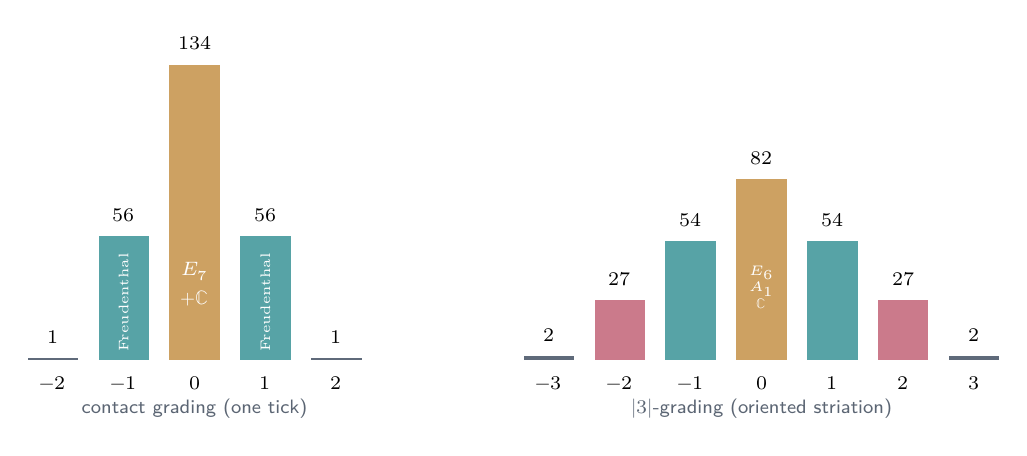
\begin{tikzpicture}[yscale=0.028,xscale=1]
  % contact grading
  \begin{scope}
    \foreach \d/\h/\c in {-2/1/ink,-1/56/teal,0/134/gold,1/56/teal,2/1/ink}{
      \fill[\c!70] (\d*0.9-0.32,0) rectangle (\d*0.9+0.32,\h);
      \node[font=\scriptsize,anchor=south] at (\d*0.9,\h+2) {$\h$};
      \node[font=\scriptsize,anchor=north] at (\d*0.9,-3) {$\d$};}
    \node[font=\sffamily\scriptsize,text=slate] at (0,-22) {contact grading (one tick)};
    \node[font=\scriptsize,text=white] at (0,40) {$E_7$};
    \node[font=\scriptsize,text=white] at (0,28) {$+\C$};
    \node[font=\tiny,text=white,rotate=90] at (-0.9,26) {Freudenthal};
    \node[font=\tiny,text=white,rotate=90] at (0.9,26) {Freudenthal};
  \end{scope}
  % |3| grading
  \begin{scope}[xshift=7.2cm]
    \foreach \d/\h/\c in {-3/2/ink,-2/27/rose,-1/54/teal,0/82/gold,1/54/teal,2/27/rose,3/2/ink}{
      \fill[\c!70] (\d*0.9-0.32,0) rectangle (\d*0.9+0.32,\h);
      \node[font=\scriptsize,anchor=south] at (\d*0.9,\h+2) {$\h$};
      \node[font=\scriptsize,anchor=north] at (\d*0.9,-3) {$\d$};}
    \node[font=\sffamily\scriptsize,text=slate] at (0,-22) {$|3|$-grading (oriented striation)};
    \node[font=\tiny,text=white,align=center] at (0,33) {$E_6$\\$A_1$\\$\C$};
  \end{scope}
\end{tikzpicture}
\caption{Two ways a clock slices $E_8$. Heights are dimensions. On the left, the
Freudenthal ``$56$'' of Section~6 appears at degree $\pm1$; on the right, the $27$ of
$E_6$ appears doubled at degree $\pm1$ and single at degree $\pm2$.}
\label{fig:gradings}
\end{figure}

This parabolic spectrum was found independently by Kraft, Regeta and Zimmermann in a
study of small varieties with group actions \cite{KRZ2020}. What is repository-specific is
the identification with the Hesse clocks and the committed structure constants.

\subsection{The cubic ladder: three steps to the top}

In the $|3|$-grading, positive degrees form a nilpotent algebra
$\g_+=\g_1\oplus\g_2\oplus\g_3$ of dimension $54+27+2=83$. It is generated by $\g_1$, and
the way it fills up is governed by the $E_6$ cubic.

\begin{result}{Theorem 5.5 (the bracket ladder) \hfill \tierC}
On the committed Chevalley bracket:
\begin{enumerate}[label=(\roman*),leftmargin=1.5em]
\item $[\g_1,\g_1]=\g_2$: $270$ nonzero pairs hit all $27$ grade-two roots, each ten times;
\item $[\g_1,\g_2]=\g_3$: $54$ nonzero pairs hit both top roots, each $27$ times;
\item the nonzero nested triple brackets exhibit exactly the $45$ triads of the cubic,
      each $12$ times, and for every signed triad $d_{ijk}$,
      $[[e_{(i,0)},e_{(j,1)}],e_{(k,a)}]=-d_{ijk}\,T_a$ for $a\in\{0,1\}$.
\end{enumerate}
So the positive part grows $54\to81\to83$, and the committed cubic is exactly the rule by
which three first-order moves reach the two-dimensional top.
\cert{w33\_20260925\_cubic\_clock\_bracket\_ladder.py}
\end{result}

\begin{figure}[htbp]
\centering
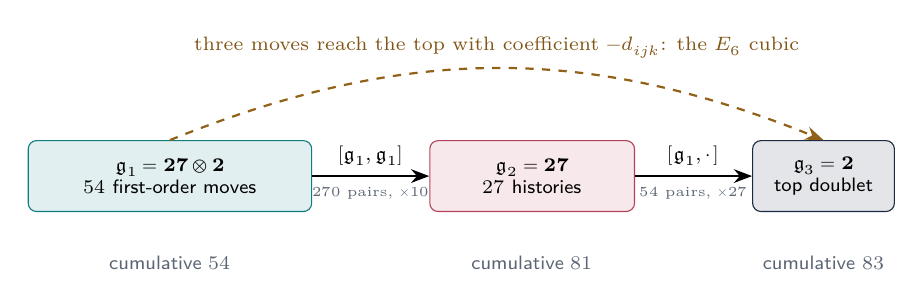
\begin{tikzpicture}[>={Stealth[length=2.3mm]},
   blk/.style={draw=#1,fill=#1!12,rounded corners=3pt,align=center,font=\sffamily\scriptsize,minimum height=9mm}]
  \node[blk=teal,minimum width=36mm] (g1) at (0,0) {$\g_1=\mathbf{27}\otimes\mathbf2$\\$54$ first-order moves};
  \node[blk=rose,minimum width=26mm] (g2) at (4.6,0) {$\g_2=\mathbf{27}$\\$27$ histories};
  \node[blk=ink,minimum width=18mm] (g3) at (8.3,0) {$\g_3=\mathbf2$\\top doublet};
  \draw[->,line width=1pt] (g1) -- node[above,font=\scriptsize]{$[\g_1,\g_1]$} node[below,font=\tiny,text=slate]{$270$ pairs, $\times10$} (g2);
  \draw[->,line width=1pt] (g2) -- node[above,font=\scriptsize]{$[\g_1,\cdot\,]$} node[below,font=\tiny,text=slate]{$54$ pairs, $\times27$} (g3);
  \node[font=\sffamily\scriptsize,text=slate] at (0,-1.1) {cumulative $54$};
  \node[font=\sffamily\scriptsize,text=slate] at (4.6,-1.1) {cumulative $81$};
  \node[font=\sffamily\scriptsize,text=slate] at (8.3,-1.1) {cumulative $83$};
  \draw[->,gold!80!black,dashed,line width=0.8pt] (g1.north) to[bend left=22] node[above,font=\scriptsize,text=gold!70!black]{three moves reach the top with coefficient $-d_{ijk}$: the $E_6$ cubic} (g3.north);
\end{tikzpicture}
\caption{The cubic ladder. First-order moves combine in pairs to histories, and histories
combine with one more move to reach the two-dimensional top. The only way three moves
reach the top is through a triad of the cubic.}
\label{fig:ladder}
\end{figure}

\begin{physical}[What it means physically: cubic time]
Read degree as ``order in time''. A first-order move is a state update; two moves compose
into a second-order \emph{history}; and three reach the top doublet, whose coefficient is
the cubic volume $N$ spanned by the three moves. In this reading the $E_6$ cubic --- in
GUT language the Yukawa coupling --- is the rule by which three independent updates
produce a net displacement of the clock. The algebra is exact; the reading is a bridge,
and it lacks what would make it physics: a Hamiltonian, a state and an energy scale.
\tierB
\end{physical}

\begin{keyidea}
One qutrit's nine histories build $E_8$ as $80+84+84$. The four Hesse clocks are four
orthogonal $A_2$'s whose glue is the tetracode; a clock tick grades $E_8$ as
$1+56+134+56+1$, an oriented clock as $2+27+54+82+54+27+2$; and $E_8$'s roots fibre
six-to-one over the forty points.
\end{keyidea}

\section{The Freudenthal 56 and a 57-dimensional light cone}
\label{sec:fts}

The contact grading of Theorem~5.4 has a $56$-dimensional layer $\g_{-1}$. In the 1950s
Hans Freudenthal showed \cite{Freudenthal} that the $56$-dimensional representation of $E_7$ carries a
remarkable structure --- a symplectic form and a quartic form --- now called a
\emph{Freudenthal triple system}. It has since turned up in the physics of black holes in
supergravity and in the entanglement of qubits. This section computes it directly from the
Hesse clock, on the committed $E_8$ basis, and finds a light cone one dimension larger.

\begin{plainwords}
Think of the $56$ as the space of ``charges'' of a black hole in a theory with many
electric and magnetic fields: $28$ electric and $28$ magnetic. The symplectic form pairs
each electric charge with its magnetic partner. The quartic form is a single number built
from all $56$ charges; in string theory its square root gives the black hole's entropy.
What we show is that the forty-point geometry, through its clock, produces exactly this
structure --- including the right signs, with nothing adjusted by hand.
\end{plainwords}

\subsection{Two clocks in one table}

Let $\theta$ be the highest root of $E_8$ and $\alpha_8$ the simple root with
$\theta=\omega_8$. The tick line's contact grading is the $\alpha_8$-coefficient $a_8$ of
a root; the striation's $|3|$-grading is its $\alpha_7$-coefficient $a_7$. Counting
roots by both at once gives Figure~\ref{fig:bigrade}.

\begin{figure}[htbp]
\centering
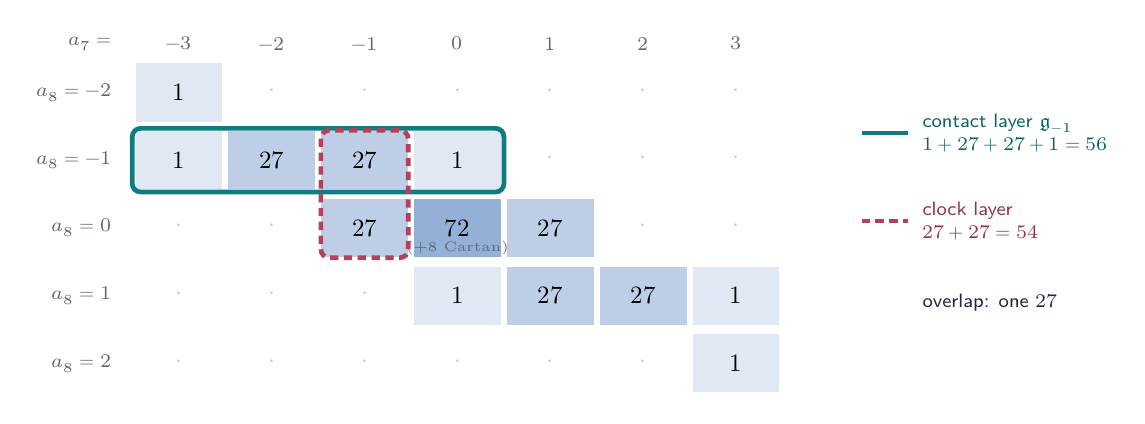
\begin{tikzpicture}[x=1.18cm,y=0.86cm,
   cell/.style={minimum width=11.4mm,minimum height=7.8mm,draw=white,line width=1.2pt,font=\small,inner sep=0pt}]
  % bigrading of the 240 roots: rows a8 = -2..2, columns a7 = -3..3
  \foreach \row/\vals [count=\r from 0] in {-2/{1,0,0,0,0,0,0},-1/{1,27,27,1,0,0,0},0/{0,0,27,72,27,0,0},1/{0,0,0,1,27,27,1},2/{0,0,0,0,0,0,1}}{
     \node[font=\scriptsize,text=slate,anchor=east] at (-0.62,-\r) {$a_8=\row$};
     \foreach \v [count=\c from 0] in \vals {
        \pgfmathsetmacro{\shade}{\v==0 ? 0 : (\v==1 ? 16 : (\v==27 ? 34 : 55))}
        \node[cell,fill=sky!\shade] at (\c,-\r) {\ifnum\v=0 \textcolor{slate!35}{$\cdot$}\else $\v$\fi};
     }}
  \foreach \a [count=\c from 0] in {-3,...,3}{\node[font=\scriptsize,text=slate] at (\c,0.72) {$\a$};}
  \node[font=\scriptsize,text=slate,anchor=east] at (-0.62,0.72) {$a_7=$};
  \node[font=\tiny,text=ink!70] at (3,-2.3) {(+8 Cartan)};
  % contact layer (row a8 = -1)
  \draw[teal,line width=1.7pt,rounded corners=3pt] (-0.5,-0.53) rectangle (3.5,-1.47);
  % clock layer (column a7 = -1)
  \draw[rose,line width=1.7pt,rounded corners=3pt,dash pattern=on 3pt off 2pt] (1.53,-0.56) rectangle (2.47,-2.44);
  % legend
  \draw[teal,line width=1.7pt] (7.35,-0.6) -- (7.85,-0.6);
  \node[anchor=west,font=\sffamily\scriptsize,text=teal!80!black,align=left] at (7.9,-0.6) {contact layer $\g_{-1}$\\$1+27+27+1=56$};
  \draw[rose,line width=1.7pt,dash pattern=on 3pt off 2pt] (7.35,-1.9) -- (7.85,-1.9);
  \node[anchor=west,font=\sffamily\scriptsize,text=rose!80!black,align=left] at (7.9,-1.9) {clock layer\\$27+27=54$};
  \node[anchor=west,font=\sffamily\scriptsize,text=ink,align=left] at (7.9,-3.1) {overlap: one $27$};
\end{tikzpicture}
\caption{The $240$ roots of $E_8$ counted by contact degree $a_8$ (rows) and clock degree
$a_7$ (columns). The Freudenthal $56$ (solid outline) and the clock's first-order $54$
(dashed outline) share exactly one $27$.}
\label{fig:bigrade}
\end{figure}

\begin{result}{Theorem 6.1 (the $56$ does not extend the $54$) \hfill \tierC}
The contact layer $a_8=-1$ sits at clock degrees $0,-1,-2,-3$ with sizes $1,27,27,1$;
the clock layer $a_7=-1$ sits at contact degrees $0,-1$ with $27$ each. The two share
exactly one $27$. The second $27$ of the Freudenthal system is the clock's
\emph{second-order} layer, and its two scalar ``poles'' are
$\alpha=e_{-\alpha_8}$ (clock degree $0$) and $\beta=e_{-(\theta-\alpha_8)}$ (clock degree
$-3$, a member of the clock's top doublet).
\cert{w33\_pass10949\_freudenthal\_quasiconformal\_clock\_cone.py}
\end{result}

\begin{boundary}[A count that misled]
A proposal circulating in the programme read the $56$ as ``the clock's $54$ plus the $2$
top directions''. The dimensions agree ($54+2=56$), but the objects do not: the $56$
contains only half of the $54$. \tierX\ (as an identification)
\end{boundary}

\subsection{The symplectic form and the Heisenberg algebra}

Brackets of two elements of the $56$ land in the one-dimensional $\g_{-2}=\C e_{-\theta}$:
$[x_i,x_j]=\Omega_{ij}\,e_{-\theta}$. On the root basis, $\Omega$ is a signed perfect
matching: $\alpha\leftrightarrow\beta$, and $X_k\leftrightarrow Y_k$ where $X_k$ and
$Y_k$ carry the \emph{same} $27$-label. Its determinant is $\pm1$, so it is unimodular
over $\Z$. Since $e_{-\theta}$ is central in $\g_{-1}\oplus\g_{-2}$, the two together form
a $57$-dimensional \emph{Heisenberg algebra} --- the same algebra that, in quantum
mechanics, is generated by positions, momenta and $i\hbar$. \tierC

\subsection{The quartic, in Freudenthal's normal form}

Define $Q(x)=\tfrac16\,\text{coefficient of }e_{-\theta}\text{ in }\ad_x^4\,e_\theta$ for
$x\in\g_{-1}$.

\begin{result}{Theorem 6.2 (the tick line is a Freudenthal triple system) \hfill \tierC}
$Q$ is an integral polynomial with $1036$ monomials (primitive coefficients
$\{1\!:\!28,\;\pm2\!:\!378,\;\pm4\!:\!630\}$), exactly invariant under all $126$ root
generators of the Levi $E_7$. Writing $x=(\alpha,X,Y,\beta)$ with $X,Y$ in the two $27$'s,
\[
\boxed{\;Q=(\alpha\beta+T(X,Y))^2-4\beta\,N(X)-4\alpha\,N(Y)+4\,T(X^\#,Y^\#)\;}
\]
where $N$ is the repository's committed $45$-triad $E_6$ cubic, $X^\#_k=\partial N/\partial
X_k$, and $T(X,Y)=\sum_k t_kX_kY_k$ with $t_k=\Omega(X_k,Y_k)\,\Omega(\alpha,\beta)$. No sign
has been adjusted by hand. Moreover $(X^\#)^\#=N(X)\,X$ and $X\cdot X^\#=3N(X)$, so $N$ is
the norm of a cubic Jordan algebra (a split Albert algebra) over $\Q$ \cite{Krutelevich}.
\cert{w33\_pass10949\_freudenthal\_quasiconformal\_clock\_cone.py}
\end{result}

The theorem makes one structural point vivid: the cubic ``history volume'' $N(X)$ of
Section~5 enters the quartic \emph{only} multiplied by a clock pole $\beta$.

\begin{physical}[Black holes and qubits]
In $\mathcal N=8$ supergravity the $56$ electric and magnetic charges of a black hole
transform under $E_{7(7)}$, and the Bekenstein--Hawking entropy is
$S=\pi\sqrt{|Q|}$ with $Q$ Cartan's quartic invariant \cite{KalloshKol}; in the
``magic'' $\mathcal N=2$ supergravity built on the octonionic Albert algebra the same
formula holds with $E_{7(-25)}$. Duff and Ferrara showed that the same quartic measures
the tripartite entanglement of seven qubits \cite{DuffFerrara}, and Borsten, Duff and
collaborators built a dictionary between black holes and qubit entanglement on it
\cite{BDDER}. Theorem~6.2 places that quartic, with its signs, inside the forty-point
geometry's clock. The two real forms named here --- $E_{7(7)}$ and $E_{7(-25)}$ --- are
exactly the two that appear, for two different reasons, in Section~7. \tierB
\end{physical}

\subsection{Jordan frames are the forty-five triads}

A \emph{frame} of a cubic Jordan algebra is a decomposition of the identity into three
orthogonal idempotents. On the committed basis, in each of four $27$-layers, the $45$ triads
of the cubic are exactly the $45$ strongly orthogonal triples of roots: the coordinate
frames. (This corrects an older reading of ``$27$ minimal idempotents'': $27$ counts the
coordinate rank-one directions; the frames are the $45$ triads.) For every coordinate
idempotent, the Peirce decomposition is $27=1+16+10$. \tierC

\subsection{The 57-dimensional light cone}

Now use the $57$-dimensional Heisenberg algebra as a space of points $p=(X,\tau)$, with
$X\in\g_{-1}$ and $\tau$ the central coordinate, and move the top vector $e_\theta$ around:
$v_p=\exp\bigl(\ad(X+\tau e_{-\theta})\bigr)\,e_\theta$.

\begin{result}{Theorem 6.3 (quasiconformal light cone) \hfill \tierC}
On the committed basis, symbolically:
\begin{enumerate}[label=(\roman*),leftmargin=1.5em]
\item the $e_{-\theta}$-component of $v_p$ is $\mathcal N(X,\tau)=\tfrac14Q(X)-\tau^2$;
\item the points compose by the Heisenberg law
      $(X_1,\tau_1)(X_2,\tau_2)=(X_1+X_2,\;\tau_1+\tau_2+\tfrac12\Omega(X_1,X_2))$;
\item the \emph{separation} $D(p,p')=\mathcal N\bigl(X-X',\;\tau-\tau'-\tfrac12\Omega(X',X)\bigr)$
      equals $B(v_p,v_{p'})/B(e_{-\theta},e_\theta)$ for the Killing form $B$;
\item the Weyl reflection $w$ exchanging $e_\theta$ and $-e_{-\theta}$ acts as an
      \emph{inversion} $\iota$, and
      \[
      D(\iota p,\iota p')=\frac{D(p,p')}{\mathcal N(p)\,\mathcal N(p')} .
      \]
\end{enumerate}
This is the G\"unaydin--Koepsell--Nicolai quasiconformal realisation of $E_8$
\cite{GKN}, now computed objectwise on the repository's basis.
\cert{w33\_pass10949\_freudenthal\_quasiconformal\_clock\_cone.py}
\end{result}

\begin{figure}[htbp]
\centering
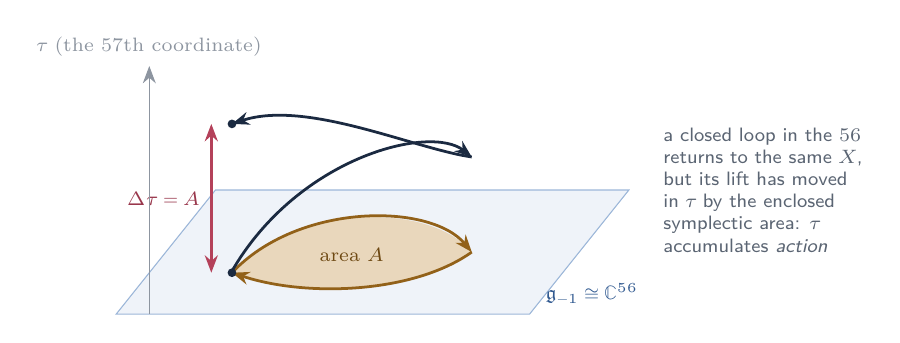
\begin{tikzpicture}[scale=1.05,>={Stealth[length=2.2mm]}]
  % Heisenberg picture: plane = 56, vertical = tau
  \fill[sky!8] (-0.4,0) -- (4.6,0) -- (5.8,1.5) -- (0.8,1.5) -- cycle;
  \draw[sky!50] (-0.4,0) -- (4.6,0) -- (5.8,1.5) -- (0.8,1.5) -- cycle;
  \node[font=\sffamily\scriptsize,text=sky!80!black] at (5.35,0.25) {$\g_{-1}\cong\C^{56}$};
  % loop in the plane
  \fill[gold!30] (1.0,0.5) .. controls (1.8,1.35) and (3.4,1.35) .. (3.9,0.75) .. controls (3.2,0.25) and (1.9,0.2) .. (1.0,0.5);
  \draw[gold!80!black,line width=1pt,->] (1.0,0.5) .. controls (1.8,1.35) and (3.4,1.35) .. (3.9,0.75);
  \draw[gold!80!black,line width=1pt,->] (3.9,0.75) .. controls (3.2,0.25) and (1.9,0.2) .. (1.0,0.5);
  \node[font=\scriptsize,text=gold!60!black] at (2.45,0.72) {area $A$};
  % lifted path
  \draw[ink,line width=1pt,->] (1.0,0.5) -- ++(0,0.02) .. controls (1.8,1.9) and (3.4,2.3) .. (3.9,1.9);
  \draw[ink,line width=1pt,->] (3.9,1.9) .. controls (3.2,2.0) and (1.9,2.6) .. (1.0,2.3);
  \draw[rose,line width=1.2pt,<->] (0.75,0.5) -- node[left,font=\scriptsize,text=rose!85!black]{$\Delta\tau=A$} (0.75,2.3);
  \fill[ink] (1.0,0.5) circle (1.5pt); \fill[ink] (1.0,2.3) circle (1.5pt);
  \draw[->,ink!50] (0,0) -- (0,3.0) node[above,font=\scriptsize]{$\tau$ (the $57$th coordinate)};
  \node[font=\sffamily\scriptsize,text=slate,align=left,anchor=west] at (6.1,1.5)
    {a closed loop in the $56$\\returns to the same $X$,\\but its lift has moved\\in $\tau$ by the enclosed\\symplectic area: $\tau$\\accumulates \emph{action}};
\end{tikzpicture}
\caption{Why the $57$th coordinate matters. In a Heisenberg group the central coordinate
of a lifted path grows by the symplectic area its projection encloses. The quasiconformal
separation $D$ depends on $\tau-\tau'$ only through this corrected difference
$\tau-\tau'-\tfrac12\Omega(X',X)$.}
\label{fig:heisenberg}
\end{figure}

\begin{physical}[What it means physically: a light cone, and its inversions]
Ordinary Minkowski space has a \emph{conformal} symmetry group, $SO(4,2)$, larger than the
Lorentz group; its most striking element is the inversion $x\mapsto x/x^2$, under which
the interval between two events transforms as
\[
(x'-y')^2=\frac{(x-y)^2}{x^2\,y^2}.
\]
Theorem~6.3(iv) is exactly this law, with the Minkowski interval replaced by the quartic
separation $D$ on a $57$-dimensional space. So $E_8$ acts on the forty-point clock's
Heisenberg algebra as a group of ``conformal'' symmetries of a quartic light cone.
The central coordinate $\tau$ plays the role of accumulated action: the same pattern met
in Section~4, where the finite present forgot a common mode that the lifted history
remembered. \tierB\ (the reading) \ \tierC\ (the formulas)
\end{physical}

\begin{keyidea}
A single tick of a Hesse clock turns $E_8$ into $1+56+134+56+1$. The $56$ is Freudenthal's
triple system, whose quartic --- computed from the committed brackets with no sign
adjusted --- is the black-hole and seven-qubit invariant; and with one more coordinate it
becomes a $57$-dimensional light cone on which $E_8$ acts by conformal-type inversions.
\end{keyidea}

\begin{boundary}
The formulas are exact, but they are the formulas of the \emph{complexified} (or split)
structure. Whether the light cone is Lorentzian --- one time direction, the rest space ---
depends on a choice of real form, which the finite field cannot see. That is the subject
of Section~7. Nothing here supplies a black hole, a charge lattice of a physical theory, or
dynamics. \tierO
\end{boundary}

\section{Real forms: where time's signature comes from}
\label{sec:real}

Every computation so far could have been done over the complex numbers --- or over
$\F_3$. But physics needs more: it needs to know which directions are \emph{time-like}
and which \emph{space-like}. Mathematically, that is the choice of a \emph{real form}.

\begin{plainwords}
A complex Lie algebra is like a map drawn without saying which way is north. A real form
chooses, for every direction, whether it behaves like a rotation (you come back to where
you started --- ``compact'', like space) or like a boost (you never come back ---
``non-compact'', like the relation between observers moving at different speeds). The
same complex $E_8$ has three real forms, and they differ precisely in how many directions
are rotation-like.
\end{plainwords}

\subsection{Three real forms of \texorpdfstring{$E_8$}{E8}}

A real form is fixed by a \emph{Cartan involution}, which splits the algebra into a
compact part $\mathfrak k$ (rotations) and a non-compact part $\mathfrak p$ (boosts). The
difference $\dim\mathfrak p-\dim\mathfrak k$ is the \emph{signature}.

\begin{figure}[htbp]
\centering
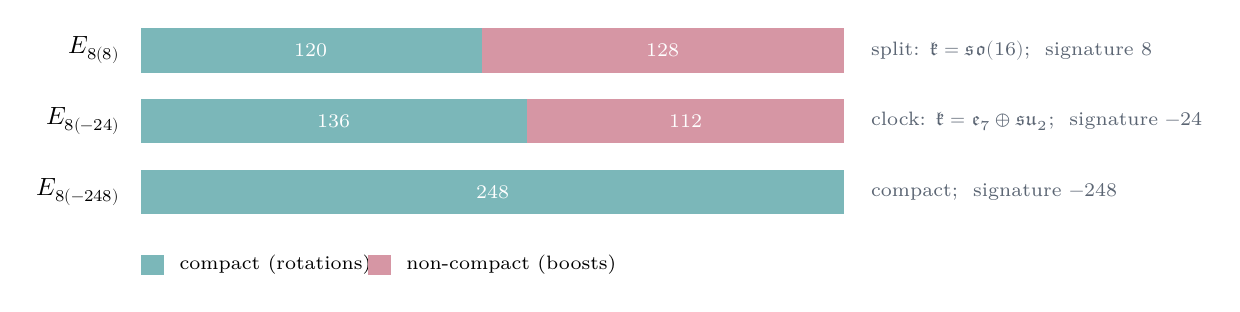
\begin{tikzpicture}[x=0.036cm,y=1cm]
  \foreach \nm/\k/\p/\sig/\lab [count=\i from 0] in
     {{$E_{8(8)}$}/120/128/8/{split: $\mathfrak k=\so(16)$},
      {$E_{8(-24)}$}/136/112/-24/{clock: $\mathfrak k=\e_7\oplus\mathfrak{su}_2$},
      {$E_{8(-248)}$}/248/0/-248/{compact}}{
    \node[anchor=east,font=\small] at (-4,-\i*0.9) {\nm};
    \fill[teal!55] (0,-\i*0.9-0.28) rectangle (\k,-\i*0.9+0.28);
    \ifnum\p>0 \fill[rose!55] (\k,-\i*0.9-0.28) rectangle (\k+\p,-\i*0.9+0.28);\fi
    \node[font=\scriptsize,text=white] at (\k/2,-\i*0.9) {$\k$};
    \ifnum\p>0 \node[font=\scriptsize,text=white] at (\k+\p/2,-\i*0.9) {$\p$};\fi
    \node[anchor=west,font=\scriptsize,text=slate] at (254,-\i*0.9) {\lab; \ signature $\sig$};
  }
  \fill[teal!55] (0,-2.85) rectangle (8,-2.6); \node[anchor=west,font=\scriptsize] at (10,-2.72) {compact (rotations)};
  \fill[rose!55] (80,-2.85) rectangle (88,-2.6); \node[anchor=west,font=\scriptsize] at (90,-2.72) {non-compact (boosts)};
\end{tikzpicture}
\caption{The three real forms of $E_8$, drawn as the split $248=\dim\mathfrak k+\dim\mathfrak p$.
The committed ``split'' form of the repository is $E_{8(8)}$; the Hesse clocks select
$E_{8(-24)}$.}
\label{fig:realforms}
\end{figure}

\subsection{A sign law, and the height twist}

On the committed Chevalley basis the Killing form obeys an exact law,
\[
K(e_\alpha,e_{-\alpha})=-60\,(-1)^{\hgt\alpha},
\]
where $\hgt\alpha$ is the height of the root (the sum of its simple-root coefficients). From
it one reads off the \emph{compact} conjugation $\sigma_c(e_\alpha)=(-1)^{\hgt\alpha}\,
\overline{e_{-\alpha}}$, verified to be an automorphism on all $30\,628$ basis pairs. The
repository's certified \emph{split} involution $\Theta$ turns out to be $\sigma_c$
composed with the \emph{height parity} $(-1)^{\hgt}=\exp(i\pi\rho^\vee)$, where $\rho^\vee$
is the Weyl co-vector. \tierC\ (\cert{w33\_pass10949\_freudenthal\_quasiconformal\_clock\_cone.py};
prior certificate \cert{w33\_e8\_split\_real\_form\_involution.py})

\subsection{The three tick lines are a Klein four-group}

The three roots $\theta$, $-(\theta-\alpha_8)$ and $-\alpha_8$ that define the tick line
and its companions sum to zero, have pairwise products $-1$, and are orthogonal to $E_6$:
they form the \emph{external} $A_2$ of $E_6\times A_2$. Each defines a parity: $(-1)^{a_8}$,
$(-1)^{a_7}$, $(-1)^{a_7+a_8}$.

\begin{result}{Theorem 7.1 (tick lines give $E_{8(-24)}$) \hfill \tierC}
Composed with $\sigma_c$, each of the three tick-line parities defines the real form
$E_{8(-24)}$. The three commute and form a Klein four-group whose simultaneous eigenspaces
decompose
\[
E_8\;=\;\underbrace{80}_{\e_6\oplus\mathfrak t_2}\;+\;56\;+\;56\;+\;56,
\]
one Freudenthal $56$ per tick line.
\cert{w33\_pass10949\_freudenthal\_quasiconformal\_clock\_cone.py}
\end{result}

\begin{figure}[htbp]
\centering
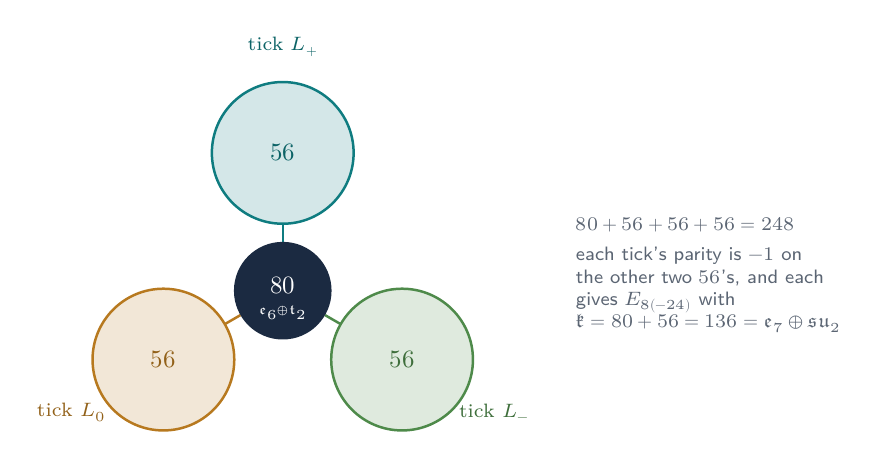
\begin{tikzpicture}[scale=1]
  \foreach \a/\c/\n in {90/teal/{L_+},210/gold/{L_0},330/sage/{L_-}}{
    \fill[\c!18,draw=\c,line width=0.9pt] (\a:1.75) circle (0.9);
    \node[font=\small\bfseries,text=\c!80!black] at (\a:1.75) {$56$};
    \node[font=\scriptsize,text=\c!80!black] at (\a:3.1) {tick $\n$};
    \draw[\c,line width=0.9pt] (\a:0.62) -- (\a:0.85);}
  \fill[ink] (0,0) circle (0.62);
  \node[text=white,font=\small\bfseries,align=center] at (0,0.07) {$80$};
  \node[text=white,font=\tiny] at (0,-0.28) {$\e_6{\oplus}\mathfrak t_2$};
  \node[font=\sffamily\scriptsize,text=slate,align=left,anchor=west] at (3.6,0.2)
    {$80+56+56+56=248$\\[3pt] each tick's parity is $-1$ on\\the other two $56$'s, and each\\gives $E_{8(-24)}$ with\\$\mathfrak k=80+56=136=\e_7\oplus\mathfrak{su}_2$};
\end{tikzpicture}
\caption{The three tick lines of a Hesse clock, and the decomposition of $E_8$ under the
Klein four-group of their parities.}
\label{fig:klein}
\end{figure}

\subsection{What each twist does to \texorpdfstring{$E_7$}{E7} and \texorpdfstring{$E_6$}{E6}}

\begin{center}
\small
\renewcommand{\arraystretch}{1.25}
\begin{tabular}{@{}llll@{}}
\toprule
\textbf{twist of $\sigma_c$} & \textbf{$E_8$} & \textbf{contact Levi $E_7$} & \textbf{$E_6$}\\
\midrule
tick $L_+$: $(-1)^{a_8}$ & $E_{8(-24)}$ & compact & compact\\
tick $L_0$: $(-1)^{a_7}$ & $E_{8(-24)}$ & $\mathbf{E_{7(-25)}}$ & compact\\
tick $L_-$: $(-1)^{a_7+a_8}$ & $E_{8(-24)}$ & $E_{7(-25)}$ & compact\\
height $(-1)^{\hgt}$ (committed split) & $E_{8(8)}$ & $\mathbf{E_{7(7)}}$ & $E_{6(2)}$\\
height $\cdot L_+$ / height $\cdot L_0$ & $E_{8(8)}$ & $E_{7(7)}$ / $E_{7(-5)}$ & $E_{6(2)}$\\
height $\cdot L_-$ & $E_{8(-24)}$ & $E_{7(-5)}$ & $E_{6(2)}$\\
\bottomrule
\end{tabular}
\end{center}

\begin{physical}[Two supergravities in one table]
$E_{7(7)}$ is the hidden symmetry (``U-duality'') of maximal $\mathcal N=8$ supergravity in
four dimensions, and $E_{8(8)}$ that of maximal supergravity in three. $E_{7(-25)}$ is the
duality group of the ``magic'' $\mathcal N=2$ supergravity built on the octonions. The
committed split form of the repository lands on the first; the Hesse clock lands on the
second. The black-hole quartic of Section~6 is the entropy formula in both. \tierB
\end{physical}

\subsection{The Lorentzian slice lives only in the clock real form}

The contact Levi $E_{7(-25)}$ has a Hermitian symmetric structure: on the $27$-dimensional
space $\mathfrak p^+=\{a_8=0,\;a_7=+1\}$ the triple product
\[
\{x,y,z\}=-[[x,\sigma_c\,y],z]
\]
makes $\mathfrak p^+$ a Hermitian Jordan triple system. A \emph{tripotent} is an element
with $\{e,e,e\}=2e$ (the normalisation used here).

\begin{result}{Theorem 7.2 (signature is a real-form datum) \hfill \tierC}
\begin{enumerate}[label=(\roman*),leftmargin=1.5em]
\item Under the clock conjugation all $27$ root vectors of $\mathfrak p^+$ are tripotents;
      under the committed split conjugation only $12$ of $27$ are.
\item For the tripotent $e$ of a triad frame, $A=\{x:\{e,x,e\}=2x\}$ with
      $x\circ y=\tfrac12\{x,e,y\}$ is a $27$-dimensional commutative Jordan algebra with
      \emph{positive-definite} trace form, inertia $(27,0,0)$: a Euclidean Jordan algebra
      of rank three --- the Albert algebra $H_3(\mathbb O)$ \cite{FarautKoranyi}.
\item For a primitive idempotent of the frame, the Peirce spaces have dimensions
      $1+16+10$, and the rank-two determinant on the $10$-dimensional Peirce-$0$ space has
      inertia $\mathbf{(1,9)}$ --- Lorentzian.
\item In the committed split form the same construction gives inertia $(5,5)$. Over $\F_3$
      the two quadrics are both of type $O^+(10,3)$ and cannot be told apart.
\end{enumerate}
\cert{w33\_pass10949\_freudenthal\_quasiconformal\_clock\_cone.py}
\end{result}

\begin{figure}[htbp]
\centering
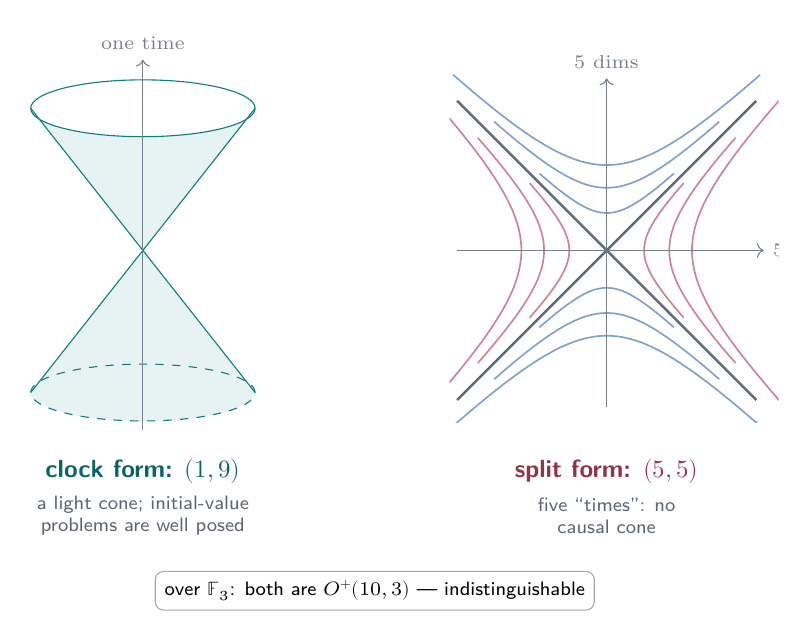
\begin{tikzpicture}[scale=0.95]
  % Lorentzian cone
  \begin{scope}
    \fill[teal!10] (0,0) -- (-1.5,1.9) arc[start angle=180,end angle=360,x radius=1.5,y radius=0.38] -- cycle;
    \fill[teal!10] (0,0) -- (-1.5,-1.9) arc[start angle=180,end angle=360,x radius=1.5,y radius=0.38] -- cycle;
    \draw[teal] (-1.5,1.9) -- (1.5,-1.9); \draw[teal] (1.5,1.9) -- (-1.5,-1.9);
    \draw[teal] (0,1.9) ellipse[x radius=1.5,y radius=0.38];
    \draw[teal,dashed] (0,-1.9) ellipse[x radius=1.5,y radius=0.38];
    \draw[->,ink!60] (0,-2.4) -- (0,2.55) node[above,font=\scriptsize]{one time};
    \node[font=\sffamily\small\bfseries,text=teal!80!black] at (0,-2.95) {clock form: $(1,9)$};
    \node[font=\sffamily\scriptsize,text=slate,align=center] at (0,-3.55) {a light cone; initial-value\\problems are well posed};
  \end{scope}
  % ultrahyperbolic (5,5): a (1,1) slice of the level sets
  \begin{scope}[xshift=6.2cm]
    \clip (-2.1,-2.3) rectangle (2.3,2.6);
    \foreach \c in {0.25,0.7,1.3}{
      \draw[rose!65,line width=0.6pt] plot[domain=-1.35:1.35,samples=40] ({sqrt(\c)*cosh(\x)},{sqrt(\c)*sinh(\x)});
      \draw[rose!65,line width=0.6pt] plot[domain=-1.35:1.35,samples=40] ({-sqrt(\c)*cosh(\x)},{sqrt(\c)*sinh(\x)});
      \draw[sky!65,line width=0.6pt] plot[domain=-1.35:1.35,samples=40] ({sqrt(\c)*sinh(\x)},{sqrt(\c)*cosh(\x)});
      \draw[sky!65,line width=0.6pt] plot[domain=-1.35:1.35,samples=40] ({sqrt(\c)*sinh(\x)},{-sqrt(\c)*cosh(\x)});}
    \draw[ink!70,line width=0.9pt] (-2,-2) -- (2,2); \draw[ink!70,line width=0.9pt] (-2,2) -- (2,-2);
    \draw[->,ink!60] (-2,0) -- (2.1,0) node[right,font=\scriptsize]{$5$ dims};
    \draw[->,ink!60] (0,-2.1) -- (0,2.3) node[above,font=\scriptsize]{$5$ dims};
  \end{scope}
  \begin{scope}[xshift=6.2cm]
    \node[font=\sffamily\small\bfseries,text=rose!80!black] at (0,-2.95) {split form: $(5,5)$};
    \node[font=\sffamily\scriptsize,text=slate,align=center] at (0,-3.55) {five ``times'': no\\causal cone};
  \end{scope}
  \node[draw=ink!40,rounded corners=3pt,fill=white,font=\sffamily\scriptsize,align=center] at (3.1,-4.55)
    {over $\F_3$: both are $O^+(10,3)$ --- indistinguishable};
\end{tikzpicture}
\caption{The same Peirce-$0$ quadric in two real forms of $E_8$. Only the real form
selected by the Hesse clock is Lorentzian.}
\label{fig:signatures}
\end{figure}

\begin{physical}[What it means physically: one time, not five]
Tegmark observed that only space-times with exactly one time direction support
predictable physics: with several, the equations of motion are ultrahyperbolic and
initial data do not determine the future \cite{Tegmark1997}. Theorem~7.2 says the finite
geometry does not decide between one time and five --- over $\F_3$ they are the same ---
but that the real form picked out by its own clock is the one-time, Lorentzian choice. The
committed split form, chosen earlier for computational convenience, is the other one.
\tierB
\end{physical}

\begin{keyidea}
Signature is not visible over a finite field. It is a choice of real form, and the Hesse
clock's tick lines make that choice: they select $E_{8(-24)}\supset E_{7(-25)}$, and with it
a Euclidean Albert algebra whose Peirce slice is a $1+9$ light cone.
\end{keyidea}

\section{The Albert algebra: ten dimensions, a spinor, and matter parity}
\label{sec:lorentz}

Section~7 produced, from the clock, a $27$-dimensional Euclidean Jordan algebra. By the
Jordan--von Neumann--Wigner classification there is exactly one such algebra that is
``exceptional'': the \emph{Albert algebra} $H_3(\mathbb O)$ of $3\times3$ Hermitian matrices
over the octonions. Since the 1930s it has been suspected of having something to do with
quantum mechanics and particle physics; this section computes its symmetries on the
committed basis and finds the Lorentz group of ten-dimensional space-time, a chiral spinor,
and the repository's own matter parity.

\begin{plainwords}
The \emph{octonions} are the largest of the four number systems in which you can divide:
the real numbers, the complex numbers, the quaternions, and the octonions, of dimensions
$1,2,4,8$. Octonions do not even obey $(ab)c=a(bc)$, yet $3\times3$ ``Hermitian'' matrices of
them --- real numbers on the diagonal, octonions above it, their conjugates below --- form a
consistent algebra of dimension $3+3\times8=27$. Its symmetries are the exceptional groups
$F_4$ and $E_6$ \cite{Baez2002}. Manogue, Dray and Wilson have recently described the
Standard Model through octonionic $E_8$ structures of this kind \cite{MDW2022}.
\end{plainwords}

\subsection{Anatomy of a \texorpdfstring{$3\times3$}{3x3} octonionic matrix}

Choose the idempotent $c=E_{11}$ (a $1$ in the top-left corner). Every element of the
algebra splits by how it behaves under multiplication by $c$ --- its \emph{Peirce
decomposition}, with eigenvalues $1$, $\tfrac12$, $0$:

\begin{figure}[htbp]
\centering
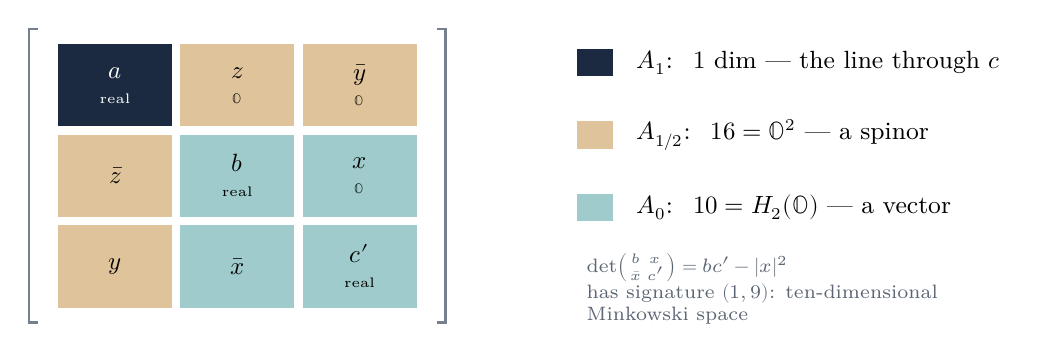
\begin{tikzpicture}[scale=1.15,
   cellbox/.style={minimum width=15mm,minimum height=11mm,draw=white,line width=1.5pt,font=\small,align=center}]
  \node[cellbox,fill=ink,text=white] at (0,0) {$a$\\[-2pt]\tiny real};
  \node[cellbox,fill=gold!45] at (1.35,0) {$z$\\[-2pt]\tiny $\mathbb O$};
  \node[cellbox,fill=gold!45] at (2.7,0) {$\bar y$\\[-2pt]\tiny $\mathbb O$};
  \node[cellbox,fill=gold!45] at (0,-1.0) {$\bar z$};
  \node[cellbox,fill=teal!40] at (1.35,-1.0) {$b$\\[-2pt]\tiny real};
  \node[cellbox,fill=teal!40] at (2.7,-1.0) {$x$\\[-2pt]\tiny $\mathbb O$};
  \node[cellbox,fill=gold!45] at (0,-2.0) {$y$};
  \node[cellbox,fill=teal!40] at (1.35,-2.0) {$\bar x$};
  \node[cellbox,fill=teal!40] at (2.7,-2.0) {$c'$\\[-2pt]\tiny real};
  \draw[ink!60,line width=1pt] (-0.85,0.62) -- (-0.95,0.62) -- (-0.95,-2.62) -- (-0.85,-2.62);
  \draw[ink!60,line width=1pt] (3.55,0.62) -- (3.65,0.62) -- (3.65,-2.62) -- (3.55,-2.62);
  % legend
  \begin{scope}[xshift=5.1cm,yshift=0.1cm]
    \fill[ink] (0,0) rectangle (0.4,0.3); \node[anchor=west,font=\small] at (0.55,0.15) {$A_1$: \ $1$ dim --- the line through $c$};
    \fill[gold!45] (0,-0.8) rectangle (0.4,-0.5); \node[anchor=west,font=\small] at (0.55,-0.65) {$A_{1/2}$: \ $16=\mathbb O^2$ --- a spinor};
    \fill[teal!40] (0,-1.6) rectangle (0.4,-1.3); \node[anchor=west,font=\small] at (0.55,-1.45) {$A_0$: \ $10=H_2(\mathbb O)$ --- a vector};
    \node[anchor=west,font=\scriptsize,text=slate,align=left] at (0,-2.35)
      {$\det\begin{psmallmatrix} b & x\\ \bar x & c'\end{psmallmatrix}=bc'-|x|^2$\\
       has signature $(1,9)$: ten-dimensional\\Minkowski space};
  \end{scope}
\end{tikzpicture}
\caption{The Peirce decomposition $27=1+16+10$ of the Albert algebra with respect to a
primitive idempotent. The lower-right $2\times2$ block is a copy of ten-dimensional
Minkowski space; the two octonions in the first row and column form a sixteen-component
spinor.}
\label{fig:peirce}
\end{figure}

That the $2\times2$ Hermitian octonionic matrices form ten-dimensional Minkowski space, with
the determinant as the Minkowski interval, is a classical observation (Sudbery; Kugo and
Townsend; Baez and Huerta), and it is the algebraic reason the superstring lives in ten
dimensions \cite{BaezHuerta,KugoTownsend}. The new content is that the forty-point clock
reaches it, on the committed basis.

\subsection{The symmetries, computed}

\begin{result}{Theorem 8.1 (the clock Albert algebra) \hfill \tierC}
For the $27$-dimensional clock algebra $A$ of Theorem~7.2:
\begin{enumerate}[label=(\roman*),leftmargin=1.5em]
\item the derivations $\mathrm{Der}(A)=\mathrm{span}\,[L_x,L_y]$ form a $52$-dimensional
      Lie algebra with negative-definite trace form $(0,52)$: the compact $F_{4(-52)}$;
\item the reduced structure algebra $\mathrm{str}_0(A)=\mathrm{Der}(A)\oplus L(A_{\mathrm{tr}=0})$
      is $78$-dimensional, obeys $[D,L_x]=L_{Dx}$ for all $52\times27$ pairs, and has
      inertia $(26,52)$: $E_{6(-26)}$;
\item the derivations fixing $c$ form a compact $36$-dimensional $\mathfrak{spin}(9)$;
      adding the nine ``boosts'' $L_y$ ($y\in A_0$, orthogonal to $e-c$) gives a
      $45$-dimensional algebra that preserves $A_0$ and its determinant of inertia $(1,9)$,
      and acts faithfully: it is $\so(1,9)$;
\item on $A_{1/2}$ the commutant of $\so(1,9)$ is one-dimensional: the $16$ is absolutely
      irreducible --- the Majorana--Weyl spinor of $\so(1,9)$.
\end{enumerate}
\cert{w33\_pass10950\_clock\_albert\_lorentz\_spinor.py}
\end{result}

\begin{center}
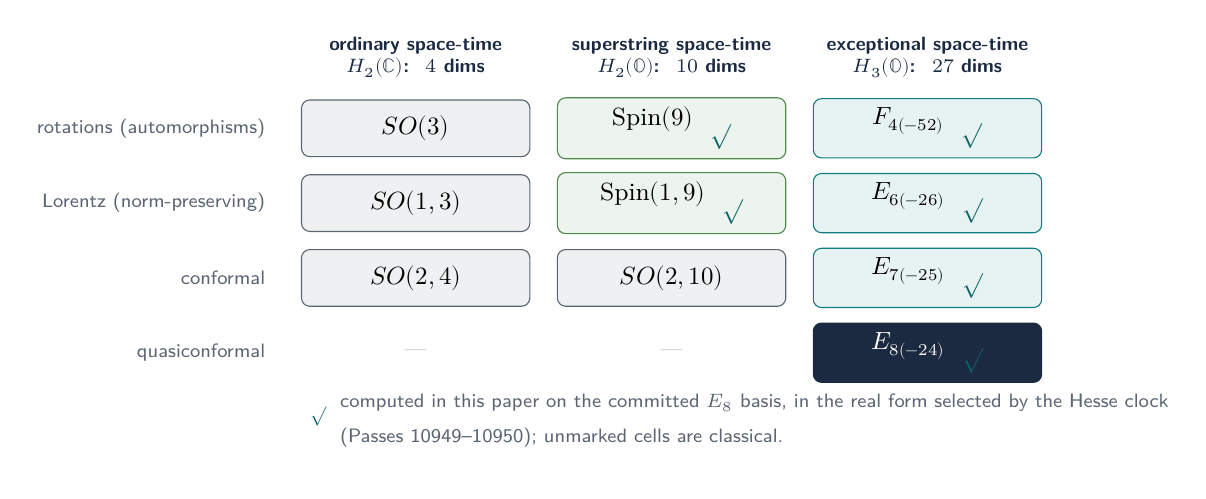
\begin{tikzpicture}[x=3.25cm,y=0.95cm,
   hd/.style={font=\sffamily\scriptsize\bfseries,align=center,text=ink},
   rw/.style={font=\sffamily\scriptsize,align=right,anchor=east,text=slate},
   cl/.style={draw=#1,fill=#1!10,rounded corners=3pt,minimum width=29mm,minimum height=7.2mm,font=\small,align=center},
   ok/.style={font=\scriptsize\bfseries,text=teal!80!black}]
  \node[hd] at (1,0.95) {ordinary space-time\\$H_2(\C)$: \ $4$ dims};
  \node[hd] at (2,0.95) {superstring space-time\\$H_2(\mathbb O)$: \ $10$ dims};
  \node[hd] at (3,0.95) {exceptional space-time\\$H_3(\mathbb O)$: \ $27$ dims};
  \foreach \lab/\y in {{rotations (automorphisms)}/0,{Lorentz (norm-preserving)}/-1,{conformal}/-2,{quasiconformal}/-3}{
     \node[rw] at (0.45,\y) {\lab};}
  % column 1
  \node[cl=slate] at (1,0) {$SO(3)$};
  \node[cl=slate] at (1,-1) {$SO(1,3)$};
  \node[cl=slate] at (1,-2) {$SO(2,4)$};
  \node[font=\scriptsize,text=slate!60] at (1,-3) {---};
  % column 2
  \node[cl=sage] at (2,0) {$\mathrm{Spin}(9)$ \ \computed};
  \node[cl=sage] at (2,-1) {$\mathrm{Spin}(1,9)$ \ \computed};
  \node[cl=slate] at (2,-2) {$SO(2,10)$};
  \node[font=\scriptsize,text=slate!60] at (2,-3) {---};
  % column 3
  \node[cl=teal] at (3,0) {$F_{4(-52)}$ \ \computed};
  \node[cl=teal] at (3,-1) {$E_{6(-26)}$ \ \computed};
  \node[cl=teal] at (3,-2) {$E_{7(-25)}$ \ \computed};
  \node[cl=ink,text=white,fill=ink] at (3,-3) {$E_{8(-24)}$ \ \computed};
  \node[font=\sffamily\scriptsize,text=slate,align=left,anchor=west] at (0.55,-4.0)
    {\computed\ \ computed in this paper on the committed $E_8$ basis, in the real form selected by the Hesse clock\\
     \phantom{\computed}\ \ (Passes 10949--10950); unmarked cells are classical.};
\end{tikzpicture}
\captionof{figure}{The ladder of space-times. A Jordan algebra of Hermitian matrices is a
space-time; its determinant is the interval. For $2\times2$ complex matrices it is
ordinary Minkowski space, for $2\times2$ octonionic matrices the ten-dimensional space of the
superstring, and for $3\times3$ octonionic matrices the $27$-dimensional ``exceptional
space-time'' of G\"unaydin \cite{Gunaydin1993}. Each has rotations, a Lorentz group, a conformal
group and (for the last) a quasiconformal group. The Hesse clock's real form of $E_8$ produces
the whole right-hand column, and the middle column inside it.}
\label{fig:spacetimes}
\end{center}

\begin{physical}[What it means physically: the clock picks the division algebra]
The last row of Freudenthal's ``magic square'' of Lie algebras can be built from the octonions
in two ways: from the division algebra $\mathbb O$, giving the chain
$F_{4(-52)}\subset E_{6(-26)}\subset E_{7(-25)}\subset E_{8(-24)}$ of automorphism, Lorentz,
conformal and quasiconformal groups of $H_3(\mathbb O)$, or from the split octonions, giving
the split forms. The Hesse clock selects the first: the \emph{division-algebra} octonions, the
ones with a positive norm, the ones that make $H_2(\mathbb O)$ a genuine Minkowski space. The
repository's earlier ``split'' choice lands on the other side. \tierC\ (the four real forms)
\ \tierB\ (the reading)
\end{physical}

\subsection{Down to four dimensions}

Choose a further splitting of the $10$ into $4+6$: time $u=e-c$, one frame direction, and
a complex line inside the octonions supplied by the complex structure of $\mathfrak p^+$
itself. The subalgebra of $\so(1,9)$ preserving the $4$ and the $6$ is $21$-dimensional,
$\so(1,3)\oplus\so(6)\cong\mathfrak{sl}(2,\C)\oplus\mathfrak{su}(4)$, and its commutant on
the $16$ is two-dimensional and contains a complex structure. Hence
\[
\mathbf{16}\;=\;(\mathbf2,\mathbf4)\;\oplus\;\overline{(\mathbf2,\mathbf4)} .
\]
\tierC\ (\cert{w33\_pass10950\_clock\_albert\_lorentz\_spinor.py})

\begin{physical}[Two readings of the same branching]
A ten-dimensional chiral spinor, seen by a four-dimensional observer, becomes four
left-handed Weyl spinors transforming as the $\mathbf4$ of $SU(4)$. If $SU(4)$ is read as
the rotation group of six hidden dimensions, this is the fermion content of maximally
supersymmetric Yang--Mills theory. If it is read as Pati--Salam colour, with lepton number
as the fourth colour, it is one generation of quarks and leptons. The branching is exact;
which reading nature uses is not decided by it. \tierB
\end{physical}

\subsection{Matter parity is a rotation by \texorpdfstring{$2\pi$}{2 pi}}

The repository carries an independent certificate for a ``matter charge'' $Q_\psi$ on the
$27$: it splits $27=16_1+10_{-2}+1_4$, and on the $45$ triads the charges fall into the
pattern $40\times(-2,1,1)+5\times(-2,-2,4)$. Matter parity is $(-1)^{Q_\psi}$: odd on the
$16$, even on the $10$ and $1$. In the Minimal Supersymmetric Standard Model a parity of
exactly this kind is what forbids the proton from decaying through dimension-four
operators.

\begin{result}{Theorem 8.2 (matter parity is the Peirce symmetry) \hfill \tierC}
For every one of the $27$ coordinate idempotents $c$, the Peirce charge
\[
Q=6L_c-2\qquad(\text{eigenvalue }4\text{ on }A_1,\;1\text{ on }A_{1/2},\;-2\text{ on }A_0)
\]
reproduces the certified spectrum of $Q_\psi$, is conserved on all $45$ triads, and
gives exactly the pattern $40\times(-2,1,1)+5\times(-2,-2,4)$. Its parity $(-1)^Q$ is the
Peirce symmetry $U_{2c-e}$, an automorphism of $A$ that is $+1$ on $A_1\oplus A_0$ and $-1$
on the spinor $A_{1/2}$. For a single-plane rotation generator $D\in\mathfrak{spin}(9)$,
$\exp(2\pi D)=U_{2c-e}$ (numerical agreement $2.7\times10^{-15}$).
\cert{w33\_pass10950\_clock\_albert\_lorentz\_spinor.py}
\end{result}

\begin{figure}[htbp]
\centering
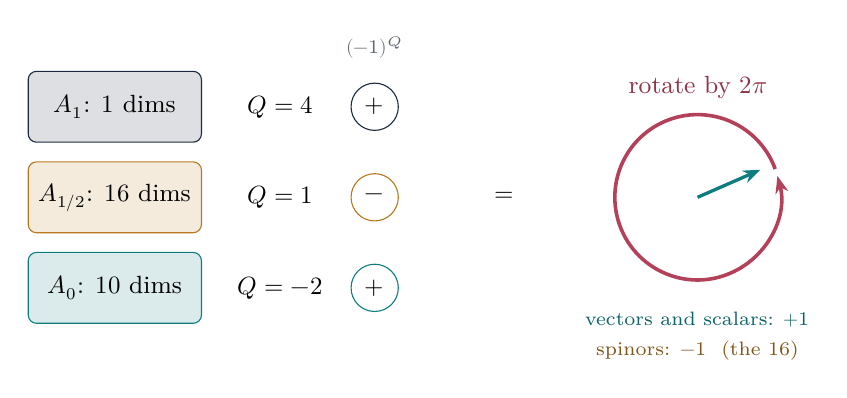
\begin{tikzpicture}[>={Stealth[length=2.2mm]}]
  % charges
  \begin{scope}
    \foreach \lab/\q/\n/\c/\s [count=\i from 0] in {{$A_1$}/4/1/ink/{+},{$A_{1/2}$}/1/16/gold/{-},{$A_0$}/-2/10/teal/{+}}{
      \node[draw=\c,fill=\c!15,rounded corners=3pt,minimum width=22mm,minimum height=9mm,font=\small,align=center] at (0,-\i*1.15) {\lab: $\n$ dims};
      \node[font=\small] at (2.1,-\i*1.15) {$Q=\q$};
      \node[circle,draw=\c,fill=white,font=\small\bfseries,minimum size=6mm,inner sep=0pt] at (3.3,-\i*1.15) {$\s$};}
    \node[font=\sffamily\scriptsize,text=slate] at (3.3,0.75) {$(-1)^Q$};
  \end{scope}
  % 2pi rotation
  \begin{scope}[xshift=7.4cm,yshift=-1.15cm]
    \draw[->,rose,line width=1.3pt] (20:1.05) arc[start angle=20,end angle=375,radius=1.05];
    \node[font=\small,text=rose!80!black] at (0,1.4) {rotate by $2\pi$};
    \draw[->,teal,line width=1.2pt] (0,0) -- (0.8,0.35);
    \node[font=\scriptsize,text=teal!80!black,align=center] at (0,-1.55) {vectors and scalars: $+1$};
    \node[font=\scriptsize,text=gold!70!black,align=center] at (0,-1.95) {spinors: $-1$ \ (the $16$)};
  \end{scope}
  \node[font=\sffamily\small] at (4.95,-1.15) {$=$};
\end{tikzpicture}
\caption{Matter parity in the clock Albert algebra: the sign that a full turn gives a spinor.}
\label{fig:parity}
\end{figure}

\begin{physical}[What it means physically]
A rotation by $2\pi$ returns every vector to itself, but multiplies every spinor by $-1$:
the mathematical root of the difference between fermions and bosons. In $SO(10)$ grand
unification it is known that matter parity can be realised by exactly such a central
element of $\mathrm{Spin}(10)$, acting as $-1$ on the matter $\mathbf{16}$ and $+1$ on the
Higgs $\mathbf{10}$ (cf.\ \cite{Martin1992}). Theorem~8.2 is the objectwise version of that fact
inside the forty-point clock: the repository's matter parity \emph{is} the $2\pi$ rotation
of the $\mathrm{Spin}(9)$ fixing a primitive idempotent. The same $27=1+10+16$ that a
GUT reads as singlet, Higgs and matter is, in the clock real form, scalar, Lorentz vector
and Weyl spinor. \tierB\ (reading) \ \tierC\ (identity)
\end{physical}

\subsection{The clock's fourth tick is the same sign}

Section~4 met a clock whose fourth tick is a sign flip. The other research track has since
shown that this is not an analogy but one spin structure, seen at both ends of the ladder.
We cite their results (certificates named) rather than re-derive them.

\begin{result}{Theorem 8.3 (clock, spin and matter parity; Passes 10951--10959) \hfill \tierC}
\begin{enumerate}[label=(\roman*),leftmargin=1.5em]
\item The negacyclic clock tick lifts uniquely to $g=\begin{psmallmatrix}0&1\\1&1\end{psmallmatrix}\in GL(2,3)$
      of order eight, with $g^4=-I$; under an explicit isomorphism $SL(2,3)\cong 2T\subset
      \mathrm{Spin}(3)$ the element $-I$ is the quaternion $-1$, the central $2\pi$ spin sign.
      \cert{w33\_pass10951\_clock\_pin\_spin\_central\_sign\_bridge.py}
\item As a signed permutation of the four clock coordinates, determinant-odd ticks exchange
      the two $D_4$ half-spin sheets and determinant-even ticks preserve them.
      \cert{w33\_pass10955\_d4\_halfspin\_clock\_bridge.py}
\item On the Albert Peirce $16$, the $\mathrm{Spin}(8)$ fixing a spatial axis splits it as
      $8_s+8_c$; an exact rational $\mathrm{Spin}(9)$ half-turn $U$ exchanges them, with
      $U^2=-I_{16}$ --- the matter-parity sign of Theorem~8.2 --- and $U^4=I_{16}$.
      \cert{w33\_pass10956\_albert\_spin8\_halfspin\_normalizer.py},
      \cert{w33\_pass10958\_exact\_albert\_mu4\_missing\_mode\_intertwiner.py}
\item One Albert $16$ cannot carry the whole order-eight clock as a $GL(2,3)$ representation;
      the minimal carrier is $16\oplus16$.
      \cert{w33\_pass10959\_albert\_clock\_extension\_obstruction.py}
\end{enumerate}
\end{result}

\begin{center}
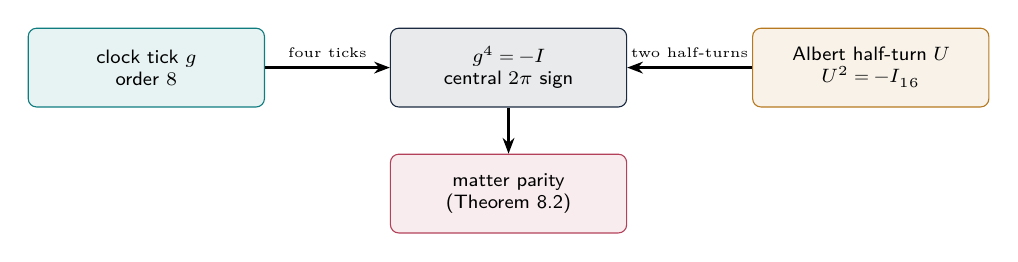
\begin{tikzpicture}[>={Stealth[length=2mm]},
   bx/.style={draw=#1,fill=#1!10,rounded corners=3pt,align=center,font=\sffamily\scriptsize,minimum height=10mm,minimum width=30mm}]
  \node[bx=teal] (g) at (0,0) {clock tick $g$\\order $8$};
  \node[bx=ink] (m) at (4.6,0) {$g^4=-I$\\central $2\pi$ sign};
  \node[bx=gold] (u) at (9.2,0) {Albert half-turn $U$\\$U^2=-I_{16}$};
  \node[bx=rose] (p) at (4.6,-1.6) {matter parity\\(Theorem 8.2)};
  \draw[->,thick] (g) -- node[above,font=\tiny]{four ticks} (m);
  \draw[->,thick] (u) -- node[above,font=\tiny]{two half-turns} (m);
  \draw[->,thick] (m) -- (p);
\end{tikzpicture}
\end{center}

\begin{boundary}
The $\so(1,9)$ here is the stabiliser of an idempotent inside $E_{6(-26)}$, an
\emph{internal} symmetry of the algebra; it is not derived to be the Lorentz group of
physical space-time, and the $2\pi$ rotation is a rotation in that internal $\mathrm{Spin}(9)$.
The identification of $Q_\psi$ with $6L_c-2$ holds up to the $W(E_6)$-transitive choice of
coordinate idempotent. Neither chirality selection, masses nor gauge dynamics follow.
\end{boundary}

\begin{keyidea}
The exceptional ladder closes: from one qutrit, through $W(3,3)$, $E_8$, a Hesse clock and
its real form, to the Albert algebra $H_3(\mathbb O)$ --- whose automorphisms are $F_4$,
whose structure group is $E_{6(-26)}$, and inside which sit ten-dimensional Minkowski space,
its Lorentz algebra $\so(1,9)$, a Majorana--Weyl spinor, and, as a rotation by $2\pi$, the
matter parity that protects the proton.
\end{keyidea}

\section{The Standard Model on forty points}
\label{sec:physics}

Sections 2--8 established exact structure. This section asks the question the programme
exists to answer: how much of the actual physics of our universe does that structure
carry? We give the answer at three levels --- what the finite geometry itself contains,
what a string compactification built on it produces, and what is still missing --- and we
end with a scorecard.

\begin{figure}[htbp]
\centering
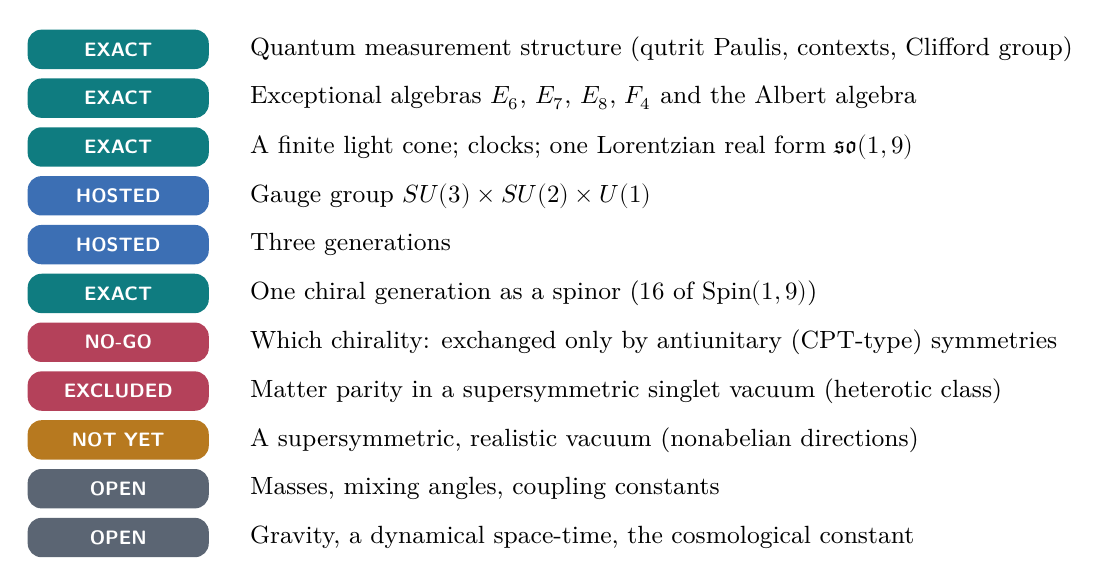
\begin{tikzpicture}[
   pill/.style={rounded corners=5pt,font=\sffamily\scriptsize\bfseries,text=white,minimum width=23mm,minimum height=5mm,inner sep=2pt},
   row/.style={anchor=west,font=\small}]
  \def\entry#1#2#3#4{%
    \node[pill,fill=#3] at (1.2,-#1*0.62) {#4};
    \node[row] at (2.75,-#1*0.62) {#2};}
  \entry{0}{Quantum measurement structure (qutrit Paulis, contexts, Clifford group)}{teal}{EXACT}
  \entry{1}{Exceptional algebras $E_6$, $E_7$, $E_8$, $F_4$ and the Albert algebra}{teal}{EXACT}
  \entry{2}{A finite light cone; clocks; one Lorentzian real form $\so(1,9)$}{teal}{EXACT}
  \entry{3}{Gauge group $SU(3)\times SU(2)\times U(1)$}{sky}{HOSTED}
  \entry{4}{Three generations}{sky}{HOSTED}
  \entry{5}{One chiral generation as a spinor ($16$ of $\mathrm{Spin}(1,9)$)}{teal}{EXACT}
  \entry{6}{Which chirality: exchanged only by antiunitary (CPT-type) symmetries}{rose}{NO-GO}
  \entry{7}{Matter parity in a supersymmetric singlet vacuum (heterotic class)}{rose}{EXCLUDED}
  \entry{8}{A supersymmetric, realistic vacuum (nonabelian directions)}{gold}{NOT YET}
  \entry{9}{Masses, mixing angles, coupling constants}{slate}{OPEN}
  \entry{10}{Gravity, a dynamical space-time, the cosmological constant}{slate}{OPEN}
\end{tikzpicture}
\caption{Scorecard. \textsf{EXACT}: a theorem or exact computation in this paper.
\textsf{HOSTED}: realised in an explicit construction built on the geometry, not forced by
it. \textsf{EXCLUDED}: exhaustively ruled out in a stated scope (Section~\ref{sec:sneutrino}).
\textsf{NO-GO}: proved impossible from inside. \textsf{OPEN}: not addressed by any exact result.}
\label{fig:scorecard}
\end{figure}

\subsection{What the finite geometry itself contains}

\paragraph{The anatomy of one symmetry.}
Pick a point $p_0$ of $\W$ and the \emph{transvection} $R$ centred on it: the symplectic
map $x\mapsto x+\langle x,v\rangle v$, of order three. It fixes the $13$ points of the plane
$p_0^\perp$ --- $p_0$ and its $12$ neighbours --- and permutes the other $27$ points in nine
orbits of three.

\begin{figure}[htbp]
\centering
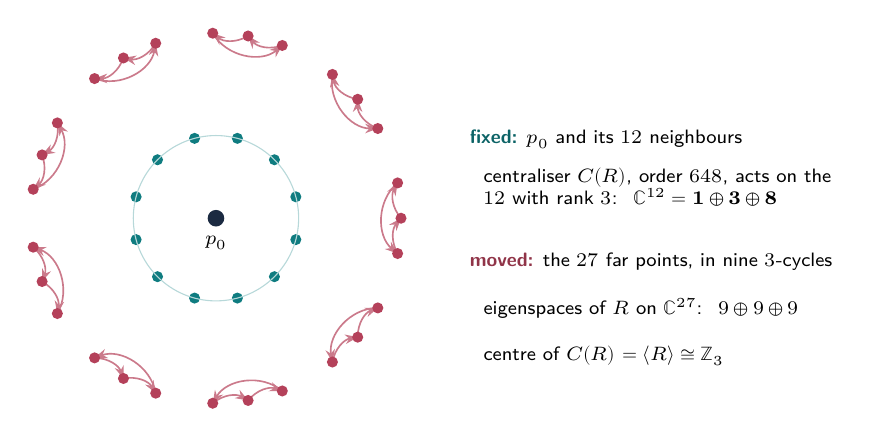
\begin{tikzpicture}[scale=1,>={Stealth[length=1.6mm]}]
  \fill[ink] (0,0) circle (3pt); \node[font=\scriptsize,anchor=north] at (0,-0.1) {$p_0$};
  \foreach \k in {0,...,11}{\fill[teal] ({30*\k+15}:1.05) circle (2pt);}
  \draw[teal!30] (0,0) circle (1.05);
  \foreach \t in {0,...,8}{
     \pgfmathsetmacro{\a}{40*\t}
     \foreach \j in {0,1,2}{
        \coordinate (q\t\j) at ({\a+(\j-1)*11}:2.35);}
     \draw[->,rose!70,line width=0.6pt] (q\t0) to[bend left=35] (q\t1);
     \draw[->,rose!70,line width=0.6pt] (q\t1) to[bend left=35] (q\t2);
     \draw[->,rose!70,line width=0.6pt] (q\t2) to[bend right=50] (q\t0);
     \foreach \j in {0,1,2}{\fill[rose] (q\t\j) circle (2pt);}}
  \node[font=\sffamily\scriptsize,align=left,anchor=west] at (3.1,1.0)
   {\textcolor{teal!80!black}{\textbf{fixed:}} $p_0$ and its $12$ neighbours};
  \node[font=\sffamily\scriptsize,align=left,anchor=west] at (3.1,0.4)
   {\ \ centraliser $C(R)$, order $648$, acts on the\\\ \ $12$ with rank $3$: \ $\C^{12}=\mathbf1\oplus\mathbf3\oplus\mathbf8$};
  \node[font=\sffamily\scriptsize,align=left,anchor=west] at (3.1,-0.55)
   {\textcolor{rose!80!black}{\textbf{moved:}} the $27$ far points, in nine $3$-cycles};
  \node[font=\sffamily\scriptsize,align=left,anchor=west] at (3.1,-1.15)
   {\ \ eigenspaces of $R$ on $\C^{27}$: \ $9\oplus9\oplus9$};
  \node[font=\sffamily\scriptsize,align=left,anchor=west] at (3.1,-1.75)
   {\ \ centre of $C(R)$ $=\langle R\rangle\cong\Z_3$};
\end{tikzpicture}
\caption{One transvection of $\W$. Its centraliser acts on the twelve fixed neighbours
with the dimensions of the Standard Model's gauge algebra, $1+3+8$, and it splits the
twenty-seven moved points into three equal eigenspaces.}
\label{fig:transvection}
\end{figure}

\begin{result}{Proposition 9.1 (the transvection spine) \hfill \tierC}
The centraliser $C(R)$ of a transvection has order $648$ (it is the point stabiliser
$3^{1+2}{:}2A_4$) and centre $\langle R\rangle\cong\Z_3$. Its permutation module on the $12$
neighbours of $p_0$ decomposes as $\mathbf1\oplus\mathbf3\oplus\mathbf8$. On the $27$ far
points, $R$ has eigenspaces $9\oplus9\oplus9$.
\cert{bt886\_standard\_model\_spine.py}
\end{result}

\begin{boundary}[How far this goes]
The dimensions $1,3,8$ are those of the Lie algebras $\mathfrak u(1)$, $\mathfrak{su}(2)$,
$\mathfrak{su}(3)$, and the corpus has sometimes read Proposition~9.1 as ``the Standard
Model gauge group follows with zero free parameters''. That is an over-read. The
$\mathbf1\oplus\mathbf3\oplus\mathbf8$ here are representations of a \emph{finite} group of
order $648$; they are not Lie algebras, they do not come with gauge fields, and nothing
fixes their couplings. The honest statement is that the local symmetry of one point of the
geometry has the \emph{shape} of the Standard Model's gauge algebra. \tierB
\end{boundary}

\paragraph{Three from the Steinberg module.}
The first homology of $\W$ (its $40$ points, $240$ edges and $160$ triangles in lines) is
$81$-dimensional and irreducible under $\PSp(4,3)$: it is the \emph{Steinberg module}, the
most rigid representation a group of Lie type has, and the logical space of the
repository's $[[240,81,3]]_3$ quantum code. \tierC\ (\cert{bt861\_code\_register\_is\_steinberg.py})

\begin{result}{Theorem 9.2 (every order-three symmetry splits matter $27+27+27$) \hfill \tierT}
Let $g\in\PSp(4,3)$ have order three. Then $g$ acts on the $81$-dimensional Steinberg
module with eigenvalues $1,\omega,\omega^2$, each with multiplicity exactly $27$.
\end{result}

\begin{proof}
The Steinberg character vanishes on every element whose order is divisible by the
defining characteristic $p=3$ (a theorem of Steinberg; see \cite{Humphreys}). So $\chi(g)=\chi(g^2)=0$, and the
multiplicity of each eigenvalue $\omega^j$ is
$\tfrac13\bigl(\chi(1)+\omega^{-j}\chi(g)+\omega^{-2j}\chi(g^2)\bigr)=81/3=27$.
\end{proof}

\begin{boundary}[Three is forced, but not selected]
Theorem~9.2 holds for \emph{every} element of order three, so it produces a threefold
splitting without choosing one. And the string-theory track (below) found that in the
explicit compactifications the number of families is the number of complex planes of the
internal torus, not a property of $\W$. We therefore record the Steinberg splitting as a
structural host for three generations, not a derivation of them. \tierB
\end{boundary}

\paragraph{The qutrit register is $SU(9)$, not $E_6$.}
One might hope that the $E_6$ of grand unification acts directly on qutrit registers.

\begin{result}{Theorem 9.3 (no Pauli $E_6$) \hfill \tierT\ \tierC}
Conjugation by the three-qutrit Pauli group splits $\mathfrak{gl}(27)$ into $729$ distinct
one-dimensional character spaces, so every conjugation-stable subalgebra is spanned by
Pauli operators. A simple Pauli-spanned Lie algebra has dimension $3^a-3^b$, i.e.\ one of
$8,24,72,80,216,240,648,720,728$. Since $\dim\e_6=78$ is not among them, $E_6$ cannot act
on a qutrit register through Pauli-stable generators.
\cert{Holotrade 1cde1f1}
\end{result}

The natural gauge algebra of the qutrit register is instead $\sll_9$ --- the $80$ of
Section~5 --- which is exactly what appears in the string construction.

\subsection{The string that carries the geometry}
\label{sec:strings}

The most developed attempt to turn this structure into physics uses the
$E_8\times E_8$ heterotic string compactified on an orbifold \cite{DHVW}: six extra dimensions curled
up as three two-dimensional tori, divided by a finite rotation group. Its advantage is
that everything is computable exactly, with a public tool, the \textsc{orbifolder}
\cite{Orbifolder}.

\begin{result}{Theorem 9.4 ($\W$ lives in the twisted sector of $E_8$) \hfill \tierC}
For the $\Z_3$ twist of the $E_8$ lattice vertex algebra, the commutator form of the
twisted-sector Pauli group equals twice the lattice form on every rung, and the resulting
commutation geometry is $\W$. The twist is anomalous on a single $E_8$ (ground-state energy
$\rho=4/9$), consistent exactly when $3\mid k$ on $E_8^{\,k}$; the $E_8^3$ orbifold is the
Niemeier lattice vertex algebra $V_{A_8^3}$ with algebra $\sll_9^{\,3}$.
\cert{Holotrade 68df33f}
\end{result}

\begin{figure}[htbp]
\centering
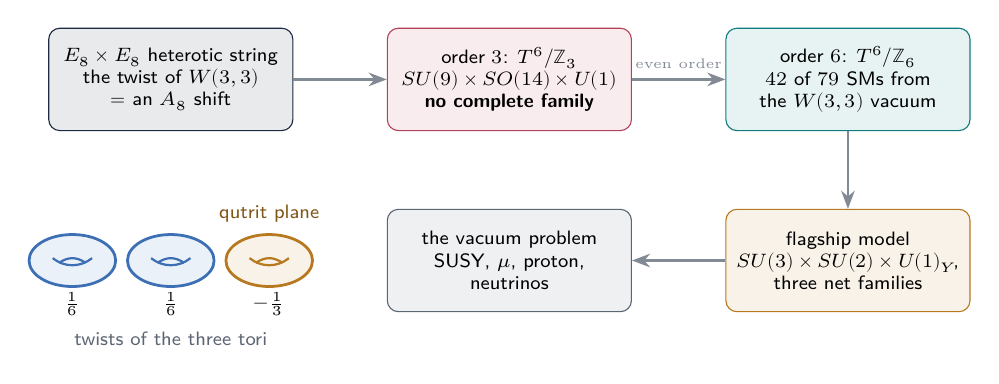
\begin{tikzpicture}[>={Stealth[length=2.3mm]},
   st/.style={draw=#1,fill=#1!10,rounded corners=4pt,align=center,font=\sffamily\scriptsize,minimum width=31mm,minimum height=13mm},
   ar/.style={->,thick,ink!55}]
  \node[st=ink] (a) at (0,0) {$E_8\times E_8$ heterotic string\\\scriptsize the twist of $\W$\\\scriptsize $=$ an $A_8$ shift};
  \node[st=rose] (b) at (4.3,0) {order $3$: $T^6/\Z_3$\\\scriptsize $SU(9)\times SO(14)\times U(1)$\\\scriptsize \textbf{no complete family}};
  \node[st=teal] (c) at (8.6,0) {order $6$: $T^6/\Z_6$\\\scriptsize $42$ of $79$ SMs from\\\scriptsize the $\W$ vacuum};
  \node[st=gold] (d) at (8.6,-2.3) {flagship model\\\scriptsize $SU(3)\times SU(2)\times U(1)_Y$,\\\scriptsize three net families};
  \node[st=slate] (e) at (4.3,-2.3) {the vacuum problem\\\scriptsize SUSY, $\mu$, proton,\\\scriptsize neutrinos};
  \draw[ar] (a) -- (b); \draw[ar] (b) -- node[above,font=\tiny]{even order} (c);
  \draw[ar] (c) -- (d); \draw[ar] (d) -- (e);
  % three tori
  \begin{scope}[xshift=0cm,yshift=-2.3cm]
    \foreach \i/\t/\c in {0/{\tfrac16}/sky,1/{\tfrac16}/sky,2/{-\tfrac13}/gold}{
       \begin{scope}[xshift=\i*1.25cm-1.25cm]
       \draw[\c,line width=1pt,fill=\c!10] (0,0) ellipse (0.55 and 0.33);
       \draw[\c,line width=0.8pt] (-0.25,0.03) .. controls (-0.1,-0.09) and (0.1,-0.09) .. (0.25,0.03);
       \draw[\c,line width=0.8pt] (-0.17,-0.03) .. controls (-0.05,0.05) and (0.05,0.05) .. (0.17,-0.03);
       \node[font=\scriptsize] at (0,-0.55) {$\t$};
       \end{scope}}
    \node[font=\sffamily\scriptsize,text=gold!70!black,align=center] at (1.25,0.6) {qutrit plane};
    \node[font=\sffamily\scriptsize,text=slate] at (0,-1.0) {twists of the three tori};
  \end{scope}
\end{tikzpicture}
\caption{The heterotic route. At order three no Wilson-line breaking completes a
Standard-Model family (a theorem); at even order the $\W$ vacuum is the most productive
source of Standard Models; the open problem is a realistic vacuum. The third torus, the
unique order-three plane, is where the Higgs lives.}
\label{fig:heterotic}
\end{figure}

\paragraph{Order three fails, for a reason.}
In the $T^6/\Z_3$ orbifold built on this twist, Wilson lines produce three-family $SU(5)$
and $SO(10)$ models; but an order-three Wilson line keeps at most one of $Q,u^c,e^c$ in each
$\mathbf{10}$, so no breaking completes a Standard-Model family. The general law: for a
$\Z_N$ orbifold, $u^c$ and $e^c$ survive together only when $N$ is even. This explains, from
first principles, why heterotic model builders moved to even-order orbifolds. An exhaustive
census of $127\,980$ classes confirms it. \tierT\ \tierC\ (Holotrade \cert{ed1eaca},
\cert{a6e1c69}, \cert{a779053})

\paragraph{Order six succeeds.}
Among the $58$ $\Z_6$-I and $61$ $\Z_6$-II shifts, the $\W$ vacuum
$SU(9)\times SO(14)\times U(1)$ is the most productive class: of $79$ inequivalent Standard
Models found in it, $42$ come from the $\Z_6$-I $\W$ vacuum. The flagship has gauge group
$SU(3)_C\times SU(2)_L\times U(1)_Y$ with three net families and no anomalies, and at one
fixed point the local gauge group is $SU(9)$ with all four simple roots of the
Standard Model's $SU(5)$ inside it: the Standard Model's unification group descends from the
twist's own $\sll_9$. \tierC\ (Holotrade \cert{5b3f3ad})

\begin{result}{Measured regularities of the $\W$ Standard Models \hfill \tierC}
\begin{itemize}[leftmargin=1.2em]
\item \textbf{The breaking is an entangling gate.} The order-three Wilson line's $\sll_9$
      holonomy is of two-qutrit controlled-$Z$ type $(5,2,2)$ in $45$ of $45$ $\Z_6$-I models,
      against a $33\%$ background (chance $\approx2.6\times10^{-22}$).
      (\cert{d772153})
\item \textbf{Two commuting holonomies cut out $SU(3)\times SU(2)$}: in all $25$ models with
      parity-type $\theta^3$, against a $30\%$ background ($\approx8.6\times10^{-14}$).
      (\cert{94df376})
\item \textbf{A heavy top is allowed}: $57$ of $60$ models admit a renormalisable top Yukawa
      coupling. (\cert{93b34e1})
\item \textbf{The Higgs sits alone in the qutrit plane}: in all $87$ $\Z_6$-I models the weak
      doublets come only from the third torus (the unique order-three plane) and colour
      triplets only from the other two; this one fact gives both the top coupling and
      \textbf{doublet--triplet splitting}, solved in $55$ of $87$ models by a
      missing-partner mechanism. (\cert{3caf15e}, \cert{a6f1cae})
\end{itemize}
\end{result}

\begin{physical}[What it means physically]
The Standard Model's most puzzling structural feature --- that the Higgs doublet is light
while its would-be colour-triplet partner, which would make protons decay, is absent --- is
here a consequence of geometry: the Higgs lives on the one internal plane whose twist has
order three, the ``qutrit plane'', and that plane carries no colour triplet. And the
symmetry breaking that produces the Standard Model is, in qutrit language, an entangling
gate. These are measured regularities of an explicit string construction, with controls;
they are not theorems about all constructions.
\end{physical}

\subsection{Where the string route stands}

A model is not a universe until it has a stable vacuum with the right low-energy
properties. Here the honest record is mixed, and it has been corrected more than once.

\begin{center}
\small
\renewcommand{\arraystretch}{1.3}
\begin{tabularx}{\textwidth}{@{}>{\raggedright\arraybackslash}p{3.0cm}X>{\raggedright\arraybackslash}p{2.4cm}@{}}
\toprule
\textbf{Requirement} & \textbf{Current exact status} & \textbf{Badge}\\
\midrule
Supersymmetric vacuum & In the doublet--triplet-solving vacuum, $F$- and $D$-flatness conflict:
one $U(1)$ direction gives every mass singlet a positive charge. Gordan's alternative
(``$D$-flat or empty superpotential, never both'') verified on all $215$ models. & \tierX\ (that vacuum)\\
$D$-flat directions & Exist in $23$ of $87$ ($\Z_6$-I) and $105$ of $128$ ($\Z_6$-II); $83$ of
the $211$ anomalous models have none. & \tierC\\
Proton stability & No supersymmetric singlet vacuum preserves a matter parity built from the
gauge torus and the space group: $0$ of $215$ (Section~\ref{sec:sneutrino}). Baryon triality is
impossible in all $215$. Heavy superpartners would need $m_t\le171$\,GeV. & \tierC\ (excluded)\\
Parity from rotations & Opens in one model ($\Z_6$II$_{23}$): unbroken, the exotics stay massless;
broken, they are heavy but no Higgs pair stays light. & \tierC\ / \tierO\\
The $\mu$ term & Arises at order $3$ or $4$ in every model; none is $\mu$-free through order
five. Must come from a vacuum symmetry. & \tierO\\
Neutrino masses & In the splitting-solving models, one to two orders of magnitude too light. & \tierO\\
\bottomrule
\end{tabularx}
\end{center}

Figure~\ref{fig:gauntlet} gathers the whole search in one picture. Each band is an exact filter; the
number is how many models or vacua pass it, and the tag names the computation that decided it.

\begin{figure}[htbp]
\centering
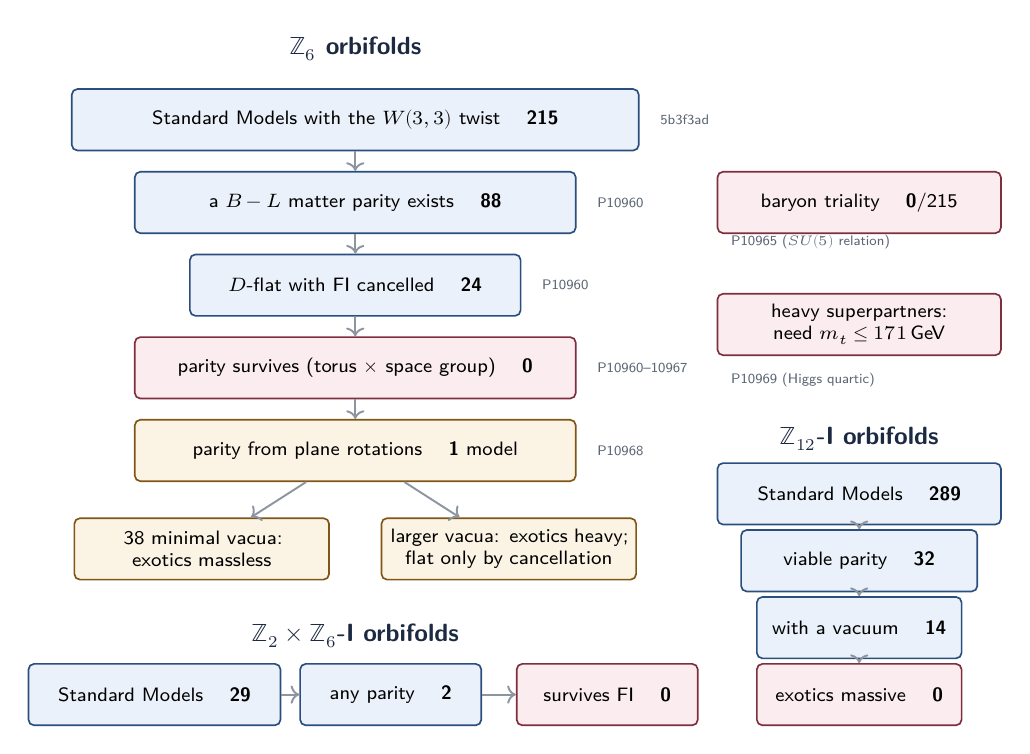
\begin{tikzpicture}[
  band/.style={draw=#1!70!black,fill=#1soft,rounded corners=2pt,minimum height=0.78cm,
               font=\sffamily\scriptsize,align=center,line width=0.6pt},
  tag/.style={font=\sffamily\tiny,text=slate,anchor=west,align=left},
  num/.style={font=\sffamily\bfseries\small,text=ink}]
  % Z6 column
  \node[font=\sffamily\bfseries\small,text=ink] at (0,0.9) {$\Z_6$ orbifolds};
  \node[band=sky,minimum width=7.2cm] (a) at (0,0) {Standard Models with the $W(3,3)$ twist \quad \textbf{215}};
  \node[band=sky,minimum width=5.6cm] (b) at (0,-1.05) {a $B-L$ matter parity exists \quad \textbf{88}};
  \node[band=sky,minimum width=4.2cm] (c) at (0,-2.1) {$D$-flat with FI cancelled \quad \textbf{24}};
  \node[band=rose,minimum width=5.6cm] (d) at (0,-3.15) {parity survives (torus $\times$ space group) \quad \textbf{0}};
  \node[band=gold,minimum width=5.6cm] (e) at (0,-4.2) {parity from plane rotations \quad \textbf{1} model};
  \node[band=gold,text width=3.0cm] (f) at (-1.95,-5.45) {38 minimal vacua:\\ exotics massless};
  \node[band=gold,text width=3.0cm] (g) at (1.95,-5.45) {larger vacua: exotics heavy;\\ flat only by cancellation};
  \foreach \u/\v in {a/b,b/c,c/d,d/e} \draw[->,ink!50,line width=0.7pt] (\u) -- (\v);
  \draw[->,ink!50,line width=0.7pt] (e) -- (f); \draw[->,ink!50,line width=0.7pt] (e) -- (g);
  \node[tag] at (3.75,0) {5b3f3ad};
  \node[tag] at (2.95,-1.05) {P10960};
  \node[tag] at (2.25,-2.1) {P10960};
  \node[tag] at (2.95,-3.15) {P10960--10967};
  \node[tag] at (2.95,-4.2) {P10968};
  % side results
  \node[band=rose,minimum width=3.6cm] (t) at (6.4,-1.05) {baryon triality \quad \textbf{0}/215};
  \node[tag] at (4.65,-1.55) {P10965 ($SU(5)$ relation)};
  \node[band=rose,minimum width=3.6cm] (h) at (6.4,-2.6) {heavy superpartners:\\ need $m_t\le171$\,GeV};
  \node[tag] at (4.65,-3.3) {P10969 (Higgs quartic)};
  % Z12 column
  \node[font=\sffamily\bfseries\small,text=ink] at (6.4,-4.05) {$\Z_{12}$-I orbifolds};
  \node[band=sky,minimum width=3.6cm] (z1) at (6.4,-4.75) {Standard Models \quad \textbf{289}};
  \node[band=sky,minimum width=3.0cm] (z2) at (6.4,-5.6) {viable parity \quad \textbf{32}};
  \node[band=sky,minimum width=2.6cm] (z3) at (6.4,-6.45) {with a vacuum \quad \textbf{14}};
  \node[band=rose,minimum width=2.6cm] (z4) at (6.4,-7.3) {exotics massive \quad \textbf{0}};
  \foreach \u/\v in {z1/z2,z2/z3,z3/z4} \draw[->,ink!50,line width=0.7pt] (\u) -- (\v);
  % Z2 x Z6 column
  \node[font=\sffamily\bfseries\small,text=ink] at (0,-6.55) {$\Z_2\times\Z_6$-I orbifolds};
  \node[band=sky,minimum width=3.2cm] (y1) at (-2.55,-7.3) {Standard Models \quad \textbf{29}};
  \node[band=sky,minimum width=2.3cm] (y2) at (0.45,-7.3) {any parity \quad \textbf{2}};
  \node[band=rose,minimum width=2.3cm] (y3) at (3.2,-7.3) {survives FI \quad \textbf{0}};
  \foreach \u/\v in {y1/y2,y2/y3} \draw[->,ink!50,line width=0.7pt] (\u) -- (\v);
\end{tikzpicture}
\caption[The vacuum gauntlet]{The vacuum gauntlet. Blue: filters passed; red: dead ends; gold: the one
door still ajar. Every count is exact (Farkas certificates, Smith normal forms, lattice tests and
integer programs), and each is regenerated by the script named in the ledger.}
\label{fig:gauntlet}
\end{figure}

\subsection{The Fayet--Iliopoulos term forces a right-handed sneutrino}
\label{sec:sneutrino}

Every model of the class has an anomalous $U(1)$, whose Fayet--Iliopoulos term must be
cancelled by giving vacuum values to some singlet fields ($D$-flatness), with $\langle
n\rangle/M_s\approx0.2$--$0.4$. Proton stability needs a \emph{matter parity} --- a $\Z_2$
under which quarks and leptons are odd and Higgs fields even --- to survive that
condensation, so the fields that condense must all be even. The earlier record found every
tested $D$-flat direction contained an odd singlet, but it had \emph{sampled} $60$ choices of
$B-L$ per model and said explicitly that this was not a proof; the raw spectra needed to
finish it were in no repository. They were recovered for this paper from the original scan
and frozen as an exact-rational ledger of all $215$ models.

\begin{result}{Theorem 9.6 (no matter parity survives the FI term) \hfill \tierC}
Over the \emph{entire} rational solution set $B-L=x_0+Nt$ of each model:
\begin{enumerate}[label=(\roman*),leftmargin=1.5em]
\item $64$ of the $88$ models with a $B-L$ direction have no $D$-flat singlet direction at all
      (an exact Farkas vector certifies that the FI term cannot be cancelled);
\item in the other $23$ $\Z_6$-I models, the singlets that are even for \emph{some} choice of
      $B-L$ are never $D$-flat (one exact Farkas vector each); the only singlets that are
      never even carry $3(B-L)=3$, i.e.\ $B-L=+1$, fixed by the Standard Model itself, and every
      $D$-flat direction uses one;
\item in the one remaining ($\Z_6$-II) model, all $304$ FI-cancelling extreme rays of the $D$-flat
      cone ($3334$ rays, computed exactly) are obstructed by an integer (Smith normal form)
      parity certificate; its never-even singlets carry $B-L=\pm1$.
\end{enumerate}
Independently, all $1024$ $\Z_2$ characters of the charge lattice that are odd on every
$q,u^c,d^c,e^c$ give no even $D$-flat direction. Controls: the same exact machinery finds
the $23+105=128$ $D$-flat models and the $88$ $B-L$ models of the earlier record.
\cert{w33\_pass10960\_matter\_even\_dflat\_closure.py}
\end{result}

\begin{figure}[htbp]
\centering
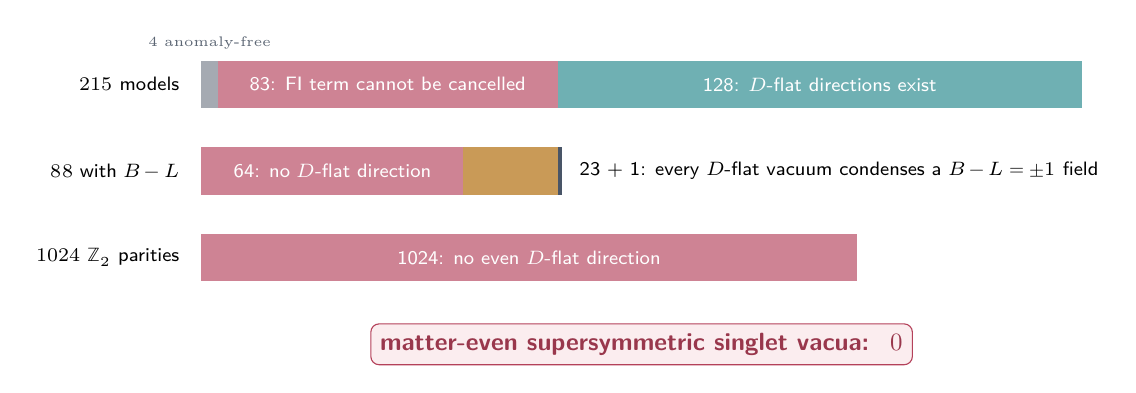
\begin{tikzpicture}[x=0.052cm,y=1cm,
   seg/.style={draw=white,line width=0.8pt},
   lab/.style={font=\sffamily\scriptsize,text=white}]
  % row 1: 215 models
  \node[anchor=east,font=\sffamily\scriptsize] at (-3,0) {$215$ models};
  \fill[slate!55] (0,-0.3) rectangle (4,0.3);
  \fill[rose!65] (4,-0.3) rectangle (87,0.3);
  \fill[teal!60] (87,-0.3) rectangle (215,0.3);
  \node[lab] at (45.5,0) {83: FI term cannot be cancelled};
  \node[lab] at (151,0) {128: $D$-flat directions exist};
  \node[font=\tiny,text=slate,anchor=south] at (2,0.32) {4 anomaly-free};
  % row 2: 88 with B-L
  \node[anchor=east,font=\sffamily\scriptsize] at (-3,-1.1) {$88$ with $B-L$};
  \fill[rose!65] (0,-1.4) rectangle (64,-0.8);
  \fill[gold!75] (64,-1.4) rectangle (87,-0.8);
  \fill[ink!80] (87,-1.4) rectangle (88,-0.8);
  \node[lab] at (32,-1.1) {64: no $D$-flat direction};
  \node[font=\sffamily\scriptsize,anchor=west] at (90,-1.1) {23 + 1: every $D$-flat vacuum condenses a $B-L=\pm1$ field};
  % row 3: Z2 characters
  \node[anchor=east,font=\sffamily\scriptsize] at (-3,-2.2) {$1024$ $\Z_2$ parities};
  \fill[rose!65] (0,-2.5) rectangle (160,-1.9);
  \node[lab] at (80,-2.2) {1024: no even $D$-flat direction};
  % verdict
  \node[draw=rose,fill=rosesoft,rounded corners=3pt,font=\sffamily\small\bfseries,text=rose!85!black]
       at (107.5,-3.3) {matter-even supersymmetric singlet vacua: \ $0$};
\end{tikzpicture}
\caption{The exhaustive closure of Theorem~9.6. Every one of the $215$ models is accounted for;
no branch leaves a matter-parity-preserving supersymmetric vacuum in singlet directions.}
\label{fig:closure}
\end{figure}

\begin{physical}[What it means physically: the sneutrino that breaks R-parity]
A singlet with $B-L=+1$ has the quantum numbers of a right-handed (s)neutrino. Theorem~9.6
says the anomalous $U(1)$ \emph{forces} such a field to condense. Martin's criterion
\cite{Martin1992} is exactly relevant here: matter parity survives the breaking of $B-L$ only
if the fields that break it have even $3(B-L)$ --- which is why realistic $SO(10)$ models
break $B-L$ with $\mathbf{126}$-type fields ($B-L=\pm2$) rather than $\mathbf{16}$-type ones
($B-L=\pm1$). In this class the FI term leaves no choice: $B-L$ is broken by one unit, and
the baryon- and lepton-number-violating couplings that matter parity was protecting are no
longer forbidden by any symmetry, at the scale of the singlet vacuum values.
\end{physical}

\paragraph{Why: one $E_6$-shaped charge.}
The obstruction has a single mechanism. In each of the $23$ models there is an exact
certificate $f$ --- a combination of the anomalous and ordinary $U(1)$ charges --- with a
prescribed physical shape: $f=\tfrac{24}{5}$ on every $q,u^c,e^c$ and $f=\tfrac85$ on every
$d^c,\ell$ (in units of a positive scale), and $f\ge0$ on every singlet that could be even.
On the singlets $f$ takes only the values $-8$, $0$ and $8$, and the negative ones are
exactly the forced $B-L=+1$ fields. Because $D$-flatness makes the $f$-charge-weighted sum of
condensates equal the (negative) FI contribution, one of them must condense. On the families
$f=4Q_\psi-\tfrac45Q_\chi$, the $U(1)$ combination of
$E_6\supset SO(10)\times U(1)_\psi\supset SU(5)\times U(1)_\chi\times U(1)_\psi$ with
$Q_\chi=4Y-5(B-L)$; the value $-8$ at $(B-L,Y)=(1,0)$ then identifies the forced field as the
right-handed-sneutrino direction of the matter-odd $\mathbf{16}_{-3}$ in the adjoint $\mathbf{78}$ of
$E_6$. \tierC\ (\cert{w33\_pass10964\_e6\_shaped\_fi\_mechanism.py}) \ \tierB\ (the $E_6$ reading)

\begin{figure}[htbp]
\centering
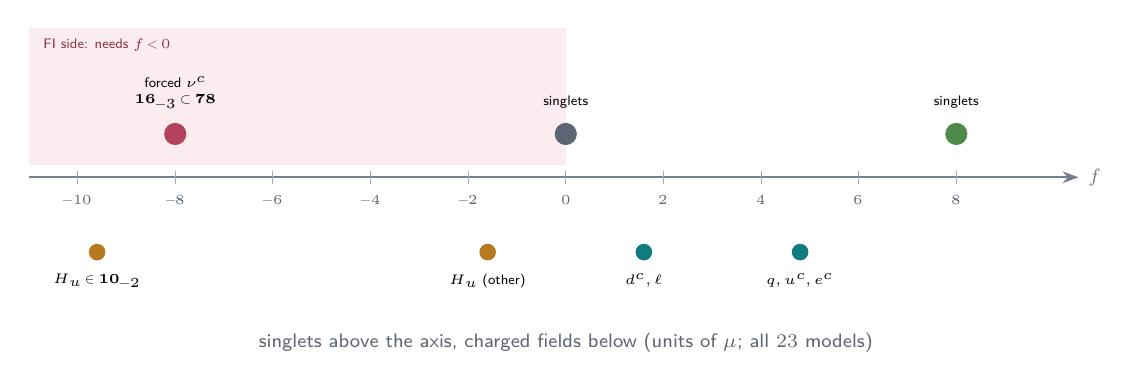
\begin{tikzpicture}[x=0.62cm,>={Stealth[length=2mm]}]
  \draw[->,ink!60,line width=0.8pt] (-11,0) -- (10.5,0) node[right,font=\scriptsize]{$f$};
  \foreach \v in {-10,-8,-6,-4,-2,0,2,4,6,8}{\draw[ink!40] (\v,-0.08) -- (\v,0.08);
     \node[font=\tiny,text=slate,anchor=north] at (\v,-0.1) {$\v$};}
  \fill[rosesoft] (-11,0.15) rectangle (0,1.9);
  \node[font=\sffamily\tiny,text=rose!80!black,anchor=north west] at (-10.9,1.88) {FI side: needs $f<0$};
  % singlets
  \foreach \v/\c/\l in {-8/rose/{forced $\nu^c$\\$\mathbf{16}_{-3}\subset\mathbf{78}$},0/slate/{singlets},8/sage/{singlets}}{
     \fill[\c] (\v,0.55) circle (4pt);
     \node[font=\sffamily\tiny,align=center,anchor=south] at (\v,0.75) {\l};}
  % families
  \fill[teal] (4.8,-0.95) circle (3pt); \node[font=\sffamily\tiny,anchor=north] at (4.8,-1.1) {$q,u^c,e^c$};
  \fill[teal] (1.6,-0.95) circle (3pt); \node[font=\sffamily\tiny,anchor=north] at (1.6,-1.1) {$d^c,\ell$};
  % higgs
  \fill[gold] (-9.6,-0.95) circle (3pt); \node[font=\sffamily\tiny,anchor=north] at (-9.6,-1.1) {$H_u\in\mathbf{10}_{-2}$};
  \fill[gold] (-1.6,-0.95) circle (3pt); \node[font=\sffamily\tiny,anchor=north] at (-1.6,-1.1) {$H_u$ (other)};
  \node[font=\sffamily\scriptsize,text=slate] at (0,-2.1) {singlets above the axis, charged fields below (units of $\mu$; all $23$ models)};
\end{tikzpicture}
\caption{The canonical certificate $f=4Q_\psi-\tfrac45Q_\chi$ on the families. Among singlets,
only the right-handed-sneutrino direction of the $E_6$ adjoint's $\mathbf{16}_{-3}$ sits on the
side that can balance the Fayet--Iliopoulos term.}
\label{fig:fline}
\end{figure}

\paragraph{The hidden sector does not rescue it.}
Theorem~9.6 covers singlets of every nonabelian group. Fields that are Standard-Model
singlets but charged under the \emph{hidden} gauge group can also condense, and their parity
can be compensated by a hidden gauge element. Pass~10962 attacks this loophole in tiers:
\begin{itemize}[leftmargin=1.2em]
\item \textbf{exact, for every hidden direction:} a parity-preserving vacuum must be $D$-flat for
      the hidden maximal torus with component-wise parity (up to a hidden torus element);
      for $32$ of the $88$ models even this relaxation has an exact Farkas certificate;
\item \textbf{exact over explicit invariant generators:} by the Luty--Taylor and Kempf--Ness
      correspondence a parity-preserving $D$-flat vacuum exists iff an FI-cancelling product of
      matter-even hidden-group invariants does; over singlets, all quadratic invariants,
      $SU(N)$ baryons and $SU(5)$ cubics, the other $55$ models close by exact Farkas vectors,
      and the last by a parity obstruction;
\item the four anomaly-free models (no FI term) admit no matter parity at all.
\end{itemize}
\tierC\ (\cert{w33\_pass10962\_hidden\_sector\_dflat\_tiers.py})

\begin{boundary}[Scope]
For the $56$ models not closed at the first tier, completeness of the invariant generators is
not proved (they contain bi-fundamental, $SU(4)$~$\mathbf6$ or $SU(5)$~$\mathbf{10}$ hidden
fields), so for them the hidden-sector statement is ``no rescue among the standard
invariants'' rather than a theorem. Whether higher-order selection rules suppress the
regenerated couplings in a particular model is not addressed. \tierO
\end{boundary}

\paragraph{The other discrete guardian is excluded too.}
Matter parity is not the only discrete symmetry that can keep the proton alive. \emph{Baryon
triality} $B_3=\exp\bigl(2\pi i(B-2Y)/3\bigr)$ (Ib\'a\~nez--Ross) forbids the baryon-number
violating couplings $u^cd^cd^c$ and $qqql$ while allowing the lepton-number violating ones.
Could the class carry it instead? As a gauge symmetry it would have to be a $\mathbb{Z}_3$
character of the $U(1)$ charge lattice, equal to $B_3$ on every quark and lepton up to a
hypercharge rotation. Pass~10965 shows that this linear system over $\mathrm{GF}(3)$ is
inconsistent in all $215$ models, and names the reason: in $214$ of them single copies obey
the exact identity
\[
  Q(u^c)+Q(e^c)=2\,Q(q)
\]
of $U(1)$ charge vectors --- the extra $U(1)$s act on the $SU(5)$ $\mathbf{10}$ through the
$\mathbf{10}$ itself. On that combination $B_3$ is $1+1-0=2$ while every hypercharge shift is
$2+0-2=0$ mod $3$, so nothing repairs it; the remaining model has an explicit integer
relation with the same property. The zero-target control is solvable in all $215$. This is
the structural reason behind Holotrade's observation that the three dimension-four operators
are locked together (b81ef8c). \tierC\ (\cert{w33\_pass10965\_baryon\_triality\_impossible.py})

\begin{plainwords}
Of the two textbook discrete symmetries that protect the proton, the first dies at the
Fayet--Iliopoulos term and the second is ruled out by the grand-unified shape of the
charges. What remains is an $R$-symmetry --- the anomaly-free $\mathbb{Z}_4^R$ of Lee, Raby,
Ratz, Ross, Schieren, Schmidt-Hoberg and Vaudrevange --- which in a string orbifold lives in the
internal rotation sector rather than in the gauge lattice. That is the one open route.
\end{plainwords}

\paragraph{The vacuum switches the forbidden couplings back on.}
Two gaps remained. First, the searches above used the $B-L$ family and $\mathbb{Z}_2$ characters
that are $\pm1$ on \emph{every} field. A matter parity only has to be $-1$ on quarks and leptons
and $+1$ on the condensate; exotic fields may carry any phase. Second, the string has discrete
symmetries of its own, the \emph{space-group selection rules}, and these are not part of the gauge
lattice. Pass~10967 closes both. It takes the most general candidate: any element of the gauge
torus times the space-group group (the point-group $\mathbb{Z}_6$, a $\mathbb{Z}_3$, and in
$\mathbb{Z}_6$-II a further $\mathbb{Z}_2\times\mathbb{Z}_2$ from fixed points). It then decides
exactly, with a Smith normal form, which singlets such an element can leave even. The answer is
unchanged: such parities exist in the same $88$ models and survive the FI term in none.

The reason is a single identity. In $290$ of the $302$ forced singlets, single copies of the fields
satisfy
\[
  Q(n)\;=\;-Q(u^cd^cd^c)\;=\;-Q(q\,\ell\,d^c)\;=\;-Q(\ell\,\ell\,e^c),
\]
which is the $SO(10)$ quartic invariant $\mathbf{16}^4$ evaluated at $\nu^c$. Each cubic is odd
under every matter parity, so $n$ is too. The string's own coupling rules then finish the argument
(Figure~\ref{fig:rpv}). In each of the $23$ $D$-flat $\mathbb{Z}_6$-I models, none of the three
$R$-parity-violating cubics is allowed at the renormalisable level. Yet all nine forced singlets
of every model appear in allowed quartics $n\,u^cd^cd^c$, $n\,q\,\ell\,d^c$ and $n\,\ell\,\ell\,e^c$.
The vacuum that supersymmetry requires turns all three back on, with strength
$\langle n\rangle/M_s\approx0.2$--$0.4$. Holotrade had noted that its class closure (b81ef8c)
held only if the vacuum breaks matter parity; this is that vacuum, named field by field.
\tierC\ (\cert{w33\_pass10967\_fi\_vacuum\_regenerates\_rpv.py})

\begin{figure}[htbp]
\centering
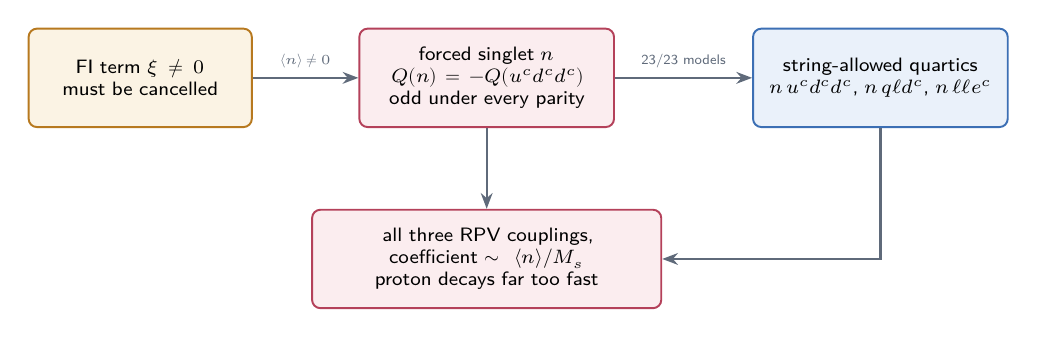
\begin{tikzpicture}[>={Stealth[length=2mm]},
  bx/.style={draw=#1,fill=#1soft,rounded corners=3pt,font=\sffamily\scriptsize,align=center,
             minimum height=1.25cm,text width=3.0cm,line width=0.7pt}]
  \node[bx=gold,text width=2.6cm] (fi) at (0,0) {FI term $\xi\neq0$\\ must be cancelled};
  \node[bx=rose] (n) at (4.4,0) {forced singlet $n$\\ $Q(n)=-Q(u^cd^cd^c)$\\ odd under every parity};
  \node[bx=sky] (q) at (9.4,0) {string-allowed quartics\\ $n\,u^cd^cd^c$, $n\,q\ell d^c$, $n\,\ell\ell e^c$};
  \node[bx=rose,text width=4.2cm] (r) at (4.4,-2.3) {all three RPV couplings, coefficient $\sim\langle n\rangle/M_s$\\ proton decays far too fast};
  \draw[->,ink!70,line width=0.8pt] (fi) -- node[above,font=\sffamily\tiny]{$\langle n\rangle\neq0$} (n);
  \draw[->,ink!70,line width=0.8pt] (n) -- node[above,font=\sffamily\tiny]{23/23 models} (q);
  \draw[->,ink!70,line width=0.8pt] (q.south) |- (r.east);
  \draw[->,ink!70,line width=0.8pt] (n.south) -- (r.north);
\end{tikzpicture}
\caption[Why supersymmetric vacua violate $R$-parity]{Why supersymmetric vacua of the class violate $R$-parity. The only fields that can cancel
the Fayet--Iliopoulos term carry exactly the conjugate charge of the three dimension-four
operators. Every string selection rule allows the resulting quartic couplings, so the vacuum turns
the cubic operators back on.}
\label{fig:rpv}
\end{figure}

\paragraph{Could heavy superpartners make it harmless?}
Another part of this programme argues that the geometry's supersymmetry is \emph{structural}, with no
light superpartners. Heavy squarks do tame $R$-parity violation, because proton decay through
$\lambda'\lambda''$ falls as $1/\tilde m^4$. With $\lambda'\sim\lambda''\sim\langle n\rangle/M_s\approx0.2$--$0.4$,
the bound $|\lambda'\lambda''|\lesssim10^{-27}(\tilde m/100\,\mathrm{GeV})^2$ needs
$\tilde m\gtrsim6\times10^{14}$--$1.2\times10^{15}$\,GeV. The Higgs sets a ceiling. Running the
Standard-Model couplings up at two loops (checked against the published three-loop value at the
Planck scale), the Higgs self-coupling turns negative at $3.2\times10^{10}$\,GeV (Figure~\ref{fig:lambda}).
Supersymmetric matching requires it to be non-negative wherever the superpartners appear. Pushing
that scale to $10^{15}$\,GeV would need a top quark of at most $171.0$\,GeV, $5.4$ standard deviations
below the measured $172.57\pm0.29$\,GeV. \tierC\ (\cert{w33\_pass10969\_rpv\_heavy\_superpartners\_vs\_higgs\_quartic.py})

\begin{figure}[htbp]
\centering
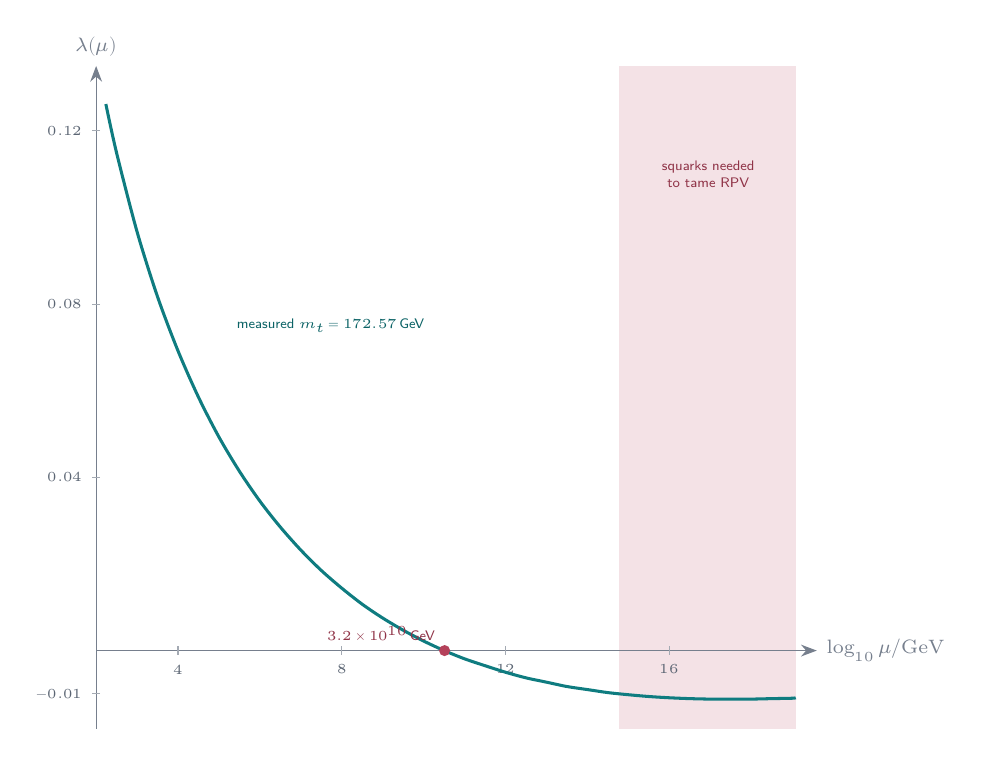
\begin{tikzpicture}[x=0.52cm,y=55cm,>={Stealth[length=2mm]}]
  \fill[rose!15] (14.78,-0.018) rectangle (19.09,0.135);
  \draw[->,ink!60] (2,0) -- (19.6,0) node[right,font=\scriptsize]{$\log_{10}\mu/\mathrm{GeV}$};
  \draw[->,ink!60] (2,-0.018) -- (2,0.135) node[above,font=\scriptsize]{$\lambda(\mu)$};
  \foreach \x in {4,8,12,16}{\draw[ink!40] (\x,0.001)--(\x,-0.001); \node[font=\tiny,anchor=north,text=slate] at (\x,-0.001) {$\x$};}
  \foreach \y in {-0.01,0.04,0.08,0.12}{\draw[ink!40] (2.1,\y)--(1.9,\y); \node[font=\tiny,anchor=east,text=slate] at (1.9,\y) {$\y$};}
  \node[font=\sffamily\tiny,text=rose!80!black,align=center] at (16.95,0.11) {squarks needed\\ to tame RPV};
  \draw[teal,line width=1.1pt] plot[smooth] coordinates {(2.237,0.1262) (2.500,0.1149) (3.000,0.0967) (3.500,0.0817) (4.000,0.0692) (4.500,0.0585) (5.000,0.0493) (5.500,0.0414) (6.000,0.0345) (6.500,0.0285) (7.000,0.0232) (7.500,0.0185) (8.000,0.0144) (8.500,0.0107) (9.000,0.0075) (9.500,0.0047) (10.000,0.0022) (10.500,0.0000) (11.000,-0.0019) (11.500,-0.0035) (12.000,-0.0050) (12.500,-0.0063) (13.000,-0.0073) (13.500,-0.0083) (14.000,-0.0090) (14.500,-0.0097) (15.000,-0.0102) (15.500,-0.0106) (16.000,-0.0109) (16.500,-0.0111) (17.000,-0.0112) (17.500,-0.0112) (18.000,-0.0112) (18.500,-0.0111) (19.000,-0.0110) (19.086,-0.0109)};
  \fill[rose] (10.51,0) circle (2pt) node[above left,font=\sffamily\tiny,text=rose!80!black]{$3.2\times10^{10}$\,GeV};
  \node[font=\sffamily\tiny,text=teal!80!black,anchor=west] at (5.2,0.075) {measured $m_t=172.57$\,GeV};
\end{tikzpicture}
\caption{The Higgs self-coupling run to high energy (two loops, NNLO matching). It turns negative
near $3\times10^{10}$\,GeV, far below the $\gtrsim6\times10^{14}$\,GeV that heavy squarks would need to
make the regenerated $R$-parity violation harmless (shaded).}
\label{fig:lambda}
\end{figure}

\paragraph{The last door: a parity made of rotations.}
The discrete groups tested so far live in the gauge lattice and the space-group rules. The orbifold
also has \emph{rotational} symmetries, turning each internal plane by its own angle, and these act on
the supersymmetry charges ($R$-symmetries). Combinations of them that leave the superpotential alone
can act as a matter parity. This reopens exactly one model, $\mathbb{Z}_6$II$_{23}$. There, $38$ minimal
supersymmetric vacua keep such a parity, with the right Higgs content; the parity is an honest symmetry
of all $1524$ couplings the string allows. But the unbroken rotation that makes these vacua flat is
the same one that forbids the exotic colour triplets from getting masses, at every order.

Larger vacua break that rotation. For the first complete parity assignment the search finds a vacuum
of $68$ directions (singlets and composites of a hidden $SU(5)$), all kept even by \emph{one} parity
element, $D$-flat with the Fayet--Iliopoulos term cancelled, in which every exotic mass matrix
reaches full rank by fifth order (exotics near $10^{15}$--$10^{16}$\,GeV), and no singlet outside the
vacuum can spoil flatness, because parity forbids it. What it cannot do is keep a Higgs pair light:
the Higgs mass matrix is full rank too. So the trade has two sides, and the class lands on one of
them in every case checked:
\begin{center}
\small
\begin{tabular}{lccc}
\toprule
vacuum & flat by symmetry & exotics & a light Higgs pair \\
\midrule
rotation unbroken ($202$ found) & yes & massless & protected \\
rotation broken, $68$ directions & no & heavy & not protected \\
rotation partly broken, $23$ directions & no & heavy & protected \\
\bottomrule
\end{tabular}
\end{center}
The last row is the \emph{approximate} rotation symmetry that the problem called for: broken at low
order for the exotics and never for one Higgs pair. It is certified exactly (a positive $D$-flat vector, one
parity element for the whole vacuum, every mass term checked against every selection rule, and every
direction outside the vacuum barred from spoiling flatness). What it lacks is flatness \emph{by
symmetry}: its superpotential is not zero, starting at sixth order with a term built from two mesons
of the hidden $SU(5)$. The branch search that makes the superpotential vanish always lands back on
the first row, with the exotic $d$-quarks massless --- $202$ times out of $202$. Whether the hidden
$SU(5)$, whose dynamics is famously able to generate a superpotential of its own, supplies the
missing cancellation is the sharpest open question the programme now has. The same analysis on a
third family of orbifolds, $\Z_2\times\Z_6$ with the $W(3,3)$ twist, finds $29$ Standard Models and
no surviving parity. \tierC\ (\cert{w33\_pass10968\_r\_symmetry\_parity\_and\_massless\_exotics.py})

\subsection{Handedness: host, not select}
\label{sec:chirality}

The weak force acts only on left-handed particles. Can $\W$ explain why?

\begin{result}{Theorem 9.5 (the chirality no-go) \hfill \tierT\ \tierC}
The two half-spin representations $S^\pm$ of the $D_5$ structure built on the
geometry are exchanged by the substrate's own outer controller $T$, which generates
$\PGSp(4,3)=\PSp(4,3){:}2=W(E_6)$ together with $\PSp(4,3)$ and has $\det T=-1$. Consequently
no invariant of the full automorphism group of $\W$ can distinguish $S^+$ from $S^-$.
\cert{w33\_pass346\_the\_chirality\_no\_go.py}
\end{result}

\begin{plainwords}
The forty-point geometry is perfectly capable of \emph{carrying} a left-handed world: the
chiral spinors are there (Section~8). What it cannot do is \emph{choose} left over right,
because one of its own symmetries swaps them. Any explanation of the handedness of the weak
force must come from outside the geometry --- from a choice of vacuum, of orientation, or of
dynamics. This is the same distinction as in Section~2: the two groups of order $51\,840$
differ precisely by whether that swapping symmetry is present.
\end{plainwords}

\begin{physical}[What it means physically: the swap is antiunitary]
Which symmetries do the swapping? For the qutrit, the determinant of a symplectic label map
decides: determinant $+1$ is a unitary Clifford operation, determinant $-1$ can only be
implemented antiunitarily (Pass~5730,
\cert{w33\_pass5727\_5730\_torsion\_family\_heisenberg.py}). The decisive statement was
proved on the $32$ orientations of a complete two-qutrit factorisation frame (Holotrade
\cert{e92a047}, \cert{frame\_chirality\_is\_reversed\_only\_by\_antiunitaries.py}): they split
$16+16$ exactly as the two half-spin weight sets of $D_5$, unitary Cliffords preserve each
half, and antiunitary ones --- and nothing else --- exchange them. The other track has since
found the same law on the clock: determinant-odd ticks exchange the two $D_4$ half-spin
sheets (Pass~10955) and are not completely positive (Pass~10952). So the geometry's
chirality is invariant under every \emph{unitary} symmetry and exchanged only by
\emph{antiunitary} ones. That is the structure of a chiral quantum theory obeying CPT:
the mirror of a chiral world is related to it by an antiunitary map, and which of the two is
called ``left'' is a convention that no internal measurement can fix. The no-go is the
finite form of this, not a defect peculiar to $\W$. \tierB\
(\cert{w33\_pass10952\_clock\_complete\_positivity\_firewall.py},
\cert{w33\_pass10955\_d4\_halfspin\_clock\_bridge.py})
\end{physical}

\begin{result}{Corollary 9.7 (one coset reverses time, acts antiunitarily, and swaps chirality) \hfill \tierT}
Fix a ``now'' (the Bell line $B$). Its stabiliser in $\PGSp(4,3)$ has order $1296$, and
its elements outside $\PSp(4,3)$ form a single coset of size $648$. That coset is exactly
\begin{enumerate}[label=(\roman*),leftmargin=1.5em]
\item the set of symmetries that \emph{reverse} the unique global orientation of the
      history graph (Theorem~4.4);
\item the set that can only be implemented \emph{antiunitarily} on qutrits (Pass~5730);
\item the set that \emph{exchange} the two chiral half-spin modules (Theorem~9.5;
      Holotrade \cert{e92a047}).
\end{enumerate}
\end{result}

\begin{proof}
Each item identifies its set with the complement of $\PSp(4,3)$ in the relevant group:
(i) is the statement of Theorem~4.4(ii) (the $648$ elements of the Bell stabiliser in
$\PSp(4,3)$ fix the orientation cycle, the other $648$ negate it); (ii) symplectic similitudes of
multiplier $+1$ lift to unitary Clifford operations and those of multiplier $-1$ only to
antiunitary ones; (iii) $\PSp(4,3)$ preserves $S^+$ and $S^-$ (they are inequivalent) while the
outer element $T$ exchanges them. Intersecting with the stabiliser of $B$ gives the same coset
in all three cases.
\end{proof}

\begin{physical}[What it means physically: a finite CPT theorem]
In quantum field theory, the CPT theorem says that the only way to relate a chiral world to
its mirror image by a symmetry is antiunitary, and that the same operation reverses the
direction of time. Corollary~9.7 is that structure, exactly, in the forty-point geometry: the
operations that reverse time's orientation are the antiunitary ones, and they are precisely
the ones that exchange left and right. Choosing an orientation of time does not choose a
chirality --- but it makes chirality a conserved label, and the world of opposite chirality
is the time-reversed one. This answers, in the finite model, the question of whether the
datum that fixes the arrow and the datum that fixes handedness are related: they live in the
same coset. \tierB
\end{physical}

\subsection{What we do not count as evidence}

The older manuscripts contain many numerical coincidences: $1/\alpha\approx137$ written as a
combination of cyclotomic values of $q=3$, spectral indices of the cosmic microwave
background, spanning-tree counts read as gravitational entropies. Some are striking. None
is derived from a dynamical principle with its uncertainties, and a finite geometry with
many natural integers can match many targets. We therefore do not use any of them as
evidence in this paper. (The value $\sin^2\theta_W=3/8$ at unification, often quoted
alongside them, is the standard prediction of any $SU(5)$ or $SO(10)$ grand unification and
is not specific to $\W$.) \tierB\ at most.

\begin{keyidea}
The geometry carries the Standard Model's shapes --- its gauge algebra's dimensions, three
equal matter sectors, a chiral spinor, a matter parity --- and a string compactification
built on its twist produces genuine three-family Standard Models whose Higgs sits in the
``qutrit plane''. It cannot choose the handedness of the weak force --- only an antiunitary,
CPT-type symmetry exchanges the two --- and, exhaustively, none of its supersymmetric singlet
vacua preserves a matter parity: the anomalous $U(1)$ forces a $B-L=\pm1$ condensate.
\end{keyidea}

\section{The machine: a computer read off the geometry}
\label{sec:machine}

The same forty points that carry $E_8$ and a light cone also describe, with no design
choices, a quantum computer: an instruction set, a memory, a network and a supply of the
non-classical resource that makes quantum computation powerful. The Holonet papers develop
this at length; here we give the parts that are exact, and mark carefully what has and has
not been built.

\begin{figure}[htbp]
\centering
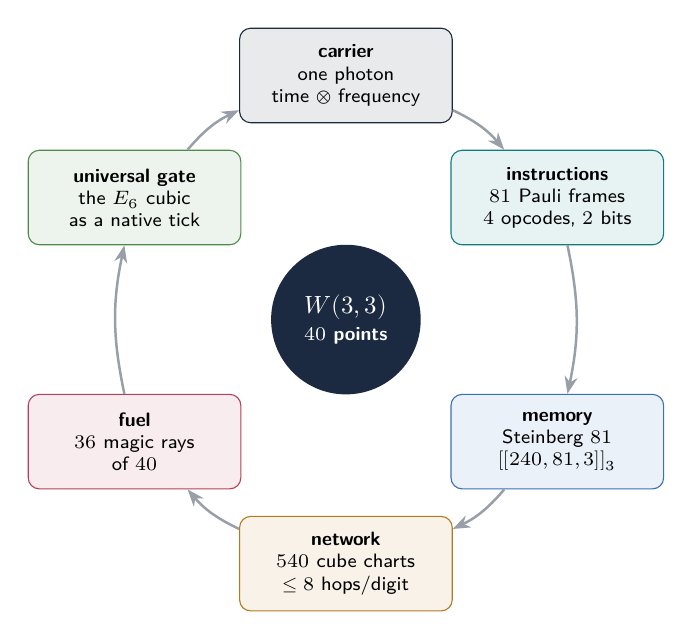
\begin{tikzpicture}[>={Stealth[length=2.2mm]},
   lay/.style={draw=#1,fill=#1!10,rounded corners=4pt,align=center,font=\sffamily\scriptsize,minimum width=27mm,minimum height=12mm}]
  \def\R{3.1}
  \foreach \nm/\c/\txt [count=\i from 0] in
     {car/ink/{\textbf{carrier}\\one photon\\time $\otimes$ frequency},
      isa/teal/{\textbf{instructions}\\$81$ Pauli frames\\$4$ opcodes, $2$ bits},
      mem/sky/{\textbf{memory}\\Steinberg $81$\\$[[240,81,3]]_3$},
      net/gold/{\textbf{network}\\$540$ cube charts\\$\le 8$ hops/digit},
      fuel/rose/{\textbf{fuel}\\$36$ magic rays\\of $40$},
      cub/sage/{\textbf{universal gate}\\the $E_6$ cubic\\as a native tick}}{
     \pgfmathsetmacro{\a}{90-60*\i}
     \node[lay=\c] (\nm) at (\a:\R) {\txt};}
  \foreach \x/\y in {car/isa,isa/mem,mem/net,net/fuel,fuel/cub,cub/car}{
     \draw[->,ink!45,line width=0.9pt] (\x) to[bend left=12] (\y);}
  \node[circle,fill=ink,text=white,font=\sffamily\small\bfseries,minimum size=19mm,align=center] at (0,0) {$\W$\\[-1pt]\scriptsize $40$ points};
\end{tikzpicture}
\caption{The Holonet stack. Every layer is a structure of $\W$ read as engineering: the
Pauli frames are the $81$ points of $\F_3^4$, the memory is the Steinberg module, the
network is the geometry's atlas of cube charts, the fuel is its set of magic states, and
the universal gate is the $E_6$ cubic of Section~5.}
\label{fig:stack}
\end{figure}

\subsection{The carrier: two qutrits in one photon}

A single photon has several independent degrees of freedom. Two of them --- which of three
\emph{time bins} it arrives in, and which of three \emph{frequency bins} it occupies ---
give two qutrits, and together the $\C^9$ on which the two-qutrit Paulis of Section~2 act.
Its path and polarisation give a second register, $\C^4$, whose $40$ Witting rays realise
$\W$ as \emph{states} (Theorem~5.3 and the box after it).

\begin{figure}[htbp]
\centering
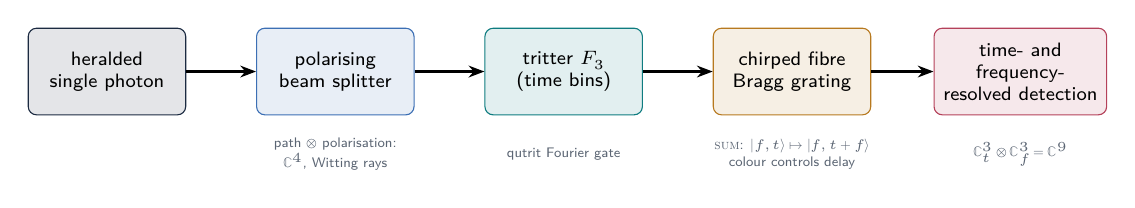
\begin{tikzpicture}[>={Stealth[length=2mm]},
   el/.style={draw=#1,fill=#1!12,rounded corners=3pt,align=center,font=\sffamily\scriptsize,minimum height=11mm,minimum width=20mm}]
  \node[el=ink] (src) at (0,0) {heralded\\single photon};
  \node[el=sky] (pbs) at (2.9,0) {polarising\\beam splitter};
  \node[el=teal] (tri) at (5.8,0) {tritter $F_3$\\(time bins)};
  \node[el=gold] (cfbg) at (8.7,0) {chirped fibre\\Bragg grating};
  \node[el=rose] (det) at (11.6,0) {time- and\\frequency-\\resolved detection};
  \draw[->,thick] (src) -- (pbs); \draw[->,thick] (pbs) -- (tri);
  \draw[->,thick] (tri) -- (cfbg); \draw[->,thick] (cfbg) -- (det);
  \node[font=\sffamily\tiny,text=slate,align=center] at (2.9,-1.05) {path $\otimes$ polarisation:\\$\C^4$, Witting rays};
  \node[font=\sffamily\tiny,text=slate,align=center] at (5.8,-1.05) {qutrit Fourier gate};
  \node[font=\sffamily\tiny,text=slate,align=center] at (8.7,-1.05) {\textsc{sum}: $\ket{f,t}\mapsto\ket{f,t+f}$\\colour controls delay};
  \node[font=\sffamily\tiny,text=slate,align=center] at (11.6,-1.05) {$\C^3_{t}\otimes\C^3_{f}=\C^9$};
\end{tikzpicture}
\caption{One photon, two qutrits. The controlled-add (\textsc{sum}) gate between the
frequency and time qutrits has been demonstrated with a single passive element, a
chirped fibre Bragg grating, at basis fidelity $0.92\pm0.01$ \cite{Imany2019}.}
\label{fig:carrier}
\end{figure}

\subsection{The instruction set}

The machine's classical control state is a \emph{Pauli frame}: a label $x\in\F_3^4$ saying
which Pauli correction is pending. There are $81$ frames. Instructions are symmetries of
the geometry: the two Fourier gates, the two phase gates, the two controlled-add gates, and
the Pauli translations.

\begin{result}{Theorem 10.1 (the complete instruction group) \hfill \tierC}
The six Clifford opcodes generate exactly $\Sp(4,3)$ (order $51\,840$); adjoining one
translation generates the affine group
\[
\mathrm{ASp}(4,3)=\F_3^4\rtimes\Sp(4,3),\qquad |\mathrm{ASp}(4,3)|=81\times51\,840=4\,199\,040 .
\]
No one or two linear opcodes suffice; exactly six triples do, so \emph{four} instructions
(three Clifford, one translation) in a \emph{two-bit} opcode field generate everything, with
worst-case program length $19$ for the best triple. The minimal arithmetic core synthesises
to $43$ logic cells at $208.86$\,MHz on an iCE40 HX8K FPGA.
\cert{holonet\_machine\_blueprint\_body.tex}, Passes 2778, 2789, 2882
\end{result}

\begin{plainwords}
Four instructions are enough to perform every one of more than four million possible
frame transformations, and no program needs more than nineteen steps. The instruction set
was not designed: it is the list of symmetries of the forty-point shape, and the
theorem says which symmetries you can leave out.
\end{plainwords}

\subsection{The fuel: matter is magic}

Clifford operations alone can be simulated efficiently on an ordinary computer; quantum
advantage needs a non-Clifford resource, usually supplied as \emph{magic states}; contextuality is what
supplies them \cite{Howard2014}.

\begin{result}{Theorem 10.2 (magic is everything except one line) \hfill \tierC}
Of the $40$ Witting rays, exactly the $4$ computational-basis rays are stabiliser states;
the other $36$ are magic. The $36$ split by stabiliser fidelity into grades $8+24+4$. A
classical $\{0,1\}$ assignment can satisfy the ``exactly one'' rule on at most $36$ of the
$40$ contexts, so the contextual fraction is exactly $1/10$; the independence number of the
collinearity graph is $7$, attained by heptads of seven rays with all pairwise overlaps $1/3$.
\cert{bt822\_magic\_census\_matter\_is\_magic.py}, \cert{bt818\_ovoid\_nogo\_theta\_gap.py}
\end{result}

\begin{figure}[htbp]
\centering
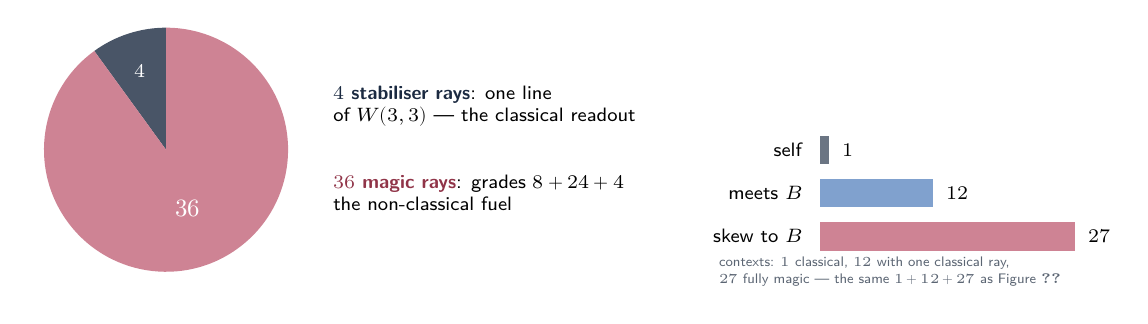
\begin{tikzpicture}
  \def\r{1.55}
  \fill[ink!80] (0,0) -- (90:\r) arc[start angle=90,end angle=126,radius=\r] -- cycle;
  \fill[rose!65] (0,0) -- (126:\r) arc[start angle=126,end angle=450,radius=\r] -- cycle;
  \node[text=white,font=\scriptsize\bfseries] at (108:1.05) {$4$};
  \node[text=white,font=\small\bfseries] at (290:0.8) {$36$};
  \node[font=\sffamily\scriptsize,anchor=west,align=left] at (2.0,0.55) {\textcolor{ink}{\textbf{$4$ stabiliser rays}}: one line\\of $\W$ --- the classical readout};
  \node[font=\sffamily\scriptsize,anchor=west,align=left] at (2.0,-0.55) {\textcolor{rose!80!black}{\textbf{$36$ magic rays}}: grades $8+24+4$\\the non-classical fuel};
  \begin{scope}[xshift=8.2cm]
    \foreach \lab/\n/\c [count=\i from 0] in {{self}/1/ink,{meets $B$}/12/sky,{skew to $B$}/27/rose}{
      \node[font=\sffamily\scriptsize,anchor=east] at (0,-\i*0.55) {\lab};
      \fill[\c!65] (0.1,-\i*0.55-0.18) rectangle (0.1+\n*0.12,-\i*0.55+0.18);
      \node[font=\scriptsize,anchor=west] at (0.15+\n*0.12,-\i*0.55) {$\n$};}
    \node[font=\sffamily\tiny,text=slate,align=left,anchor=west] at (-1.3,-1.55) {contexts: $1$ classical, $12$ with one classical ray,\\$27$ fully magic --- the same $1+12+27$ as Figure~\ref{fig:bellview}};
  \end{scope}
\end{tikzpicture}
\caption{The machine's quantum resource is the geometry itself: remove one line and every
remaining point is a magic state.}
\label{fig:magic}
\end{figure}

\paragraph{The cubic gate.}
Clifford gates are ``degree two'': they act on frame labels by linear symplectic maps and
on phases by quadratic forms. The classical continuous-variable theorem of Lloyd and
Braunstein \cite{LloydBraunstein} says that quadratic operations plus a single cubic one are universal. In
Section~5 the cubic appeared as the $E_6$ form $N$, the rule by which three first-order moves
reach the top of the ladder. Pass~10947 compiles that signed cubic into a native gate on a
seven-qutrit virtual machine: ten operations in seven parallel layers, both ancillas returned
to zero. \tierC\ (\cert{w33\_pass10947\_five\_front\_execution.py}) The same object is,
in the language of Section~5, the Yukawa coupling of $E_6$ unification, and in the language of
this section, the machine's universal non-Clifford gate. \tierB

\subsection{Memory and error correction}

\begin{result}{Theorem 10.3 (the memory is the Steinberg module) \hfill \tierC}
The CSS code $[[240,81,3]]_3$ on the edges of $\W$, with distances $(d_X,d_Z)=(3,4)$,
stores its $81$ logical qutrits in $H_1(\W)$, which is the irreducible Steinberg module of
$\PSp(4,3)$. By Schur's lemma any symmetry-covariant logical error acts as a scalar.
Separately, a ternary Golay $[[11,1,5]]_3$ lane with two verified syndrome rounds has $552$
fault locations in a declared model, $2\,576\,205$ malignant fault triples, and a conservative
threshold crossing at $p\approx5.32\times10^{-4}$.
\cert{bt861\_code\_register\_is\_steinberg.py}, \cert{w33\_pass10947\_five\_front\_execution.py}
\end{result}

\subsection{The network}

\begin{figure}[htbp]
\centering
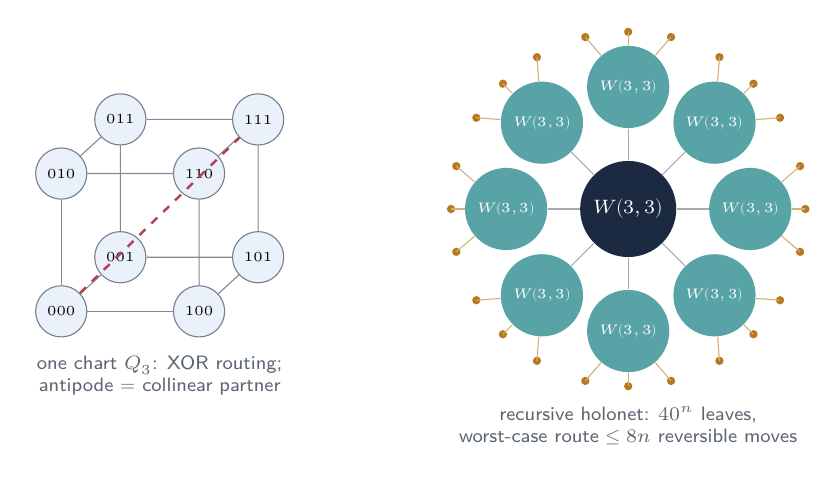
\begin{tikzpicture}[>={Stealth[length=1.8mm]},
   v/.style={circle,draw=ink!60,fill=skysoft,inner sep=0pt,minimum size=6.5mm,font=\tiny}]
  % cube chart
  \begin{scope}[scale=1.25]
    \node[v] (000) at (0,0) {000}; \node[v] (100) at (1.4,0) {100};
    \node[v] (010) at (0,1.4) {010}; \node[v] (110) at (1.4,1.4) {110};
    \node[v] (001) at (0.6,0.55) {001}; \node[v] (101) at (2.0,0.55) {101};
    \node[v] (011) at (0.6,1.95) {011}; \node[v] (111) at (2.0,1.95) {111};
    \foreach \a/\b in {000/100,000/010,100/110,010/110,001/101,001/011,101/111,011/111,000/001,100/101,010/011,110/111}{\draw[ink!55] (\a) -- (\b);}
    \draw[rose,dashed,line width=0.9pt] (000) -- (111);
    \node[font=\sffamily\scriptsize,text=slate,align=center] at (1.0,-0.65) {one chart $Q_3$: XOR routing;\\antipode $=$ collinear partner};
  \end{scope}
  % fractal
  \begin{scope}[xshift=7.2cm,yshift=1.3cm]
    \node[circle,fill=ink,text=white,minimum size=11mm,font=\scriptsize] (c) at (0,0) {$\W$};
    \foreach \k in {0,...,7}{
      \pgfmathsetmacro{\a}{\k*45}
      \node[circle,fill=teal!70,text=white,minimum size=6.5mm,font=\tiny] (s\k) at (\a:1.55) {$\W$};
      \draw[ink!40] (c) -- (s\k);
      \foreach \j in {-1,0,1}{\fill[gold] (\a+\j*14:2.25) circle (1.5pt); \draw[gold!60] (s\k) -- (\a+\j*14:2.25);}}
    \node[font=\sffamily\scriptsize,text=slate,align=center] at (0,-2.75) {recursive holonet: $40^n$ leaves,\\worst-case route $\le 8n$ reversible moves};
  \end{scope}
\end{tikzpicture}
\caption{Left: a local routing chart. Each of the $540$ pairs of disjoint lines of $\W$
carries a cube of eight points with XOR addressing. Right: substituting a copy of $\W$ at
every point gives a network with $40^n$ leaves and logarithmic routing.}
\label{fig:network}
\end{figure}

$\W$ contains exactly $540$ pairs of disjoint lines; each pair's eight points carry the
cube graph $Q_3$, in which the antipode of a vertex is its unique collinear partner. The
charts are glued along the $1620$ apartments of the Tits building of $\Sp(4,3)$. A route
needs at most $3$ in-chart moves plus $5$ chart hops, so each digit of a recursive address
costs at most $8$ reversible moves. \tierC\ (\cert{bt773\_involution\_cube\_theorem.py}, \cert{bt777\_hypercube\_chart\_web.py},
\cert{bt827\_holonet\_fractal\_architecture.py})

\begin{boundary}[What is measured, what is proved, what is not built]
\textbf{Measured in a laboratory (prior art):} the single-photon time--frequency \textsc{sum}
gate, fidelity $0.92\pm0.01$ \cite{Imany2019}. \textbf{Proved exactly:} the group theory, the
instruction semantics, reachability, code parameters, routing bounds, and FPGA synthesis
figures. \textbf{Not built:} an integrated device; a magic-state injection circuit with a
threshold; a physical demonstration of the network. The machine is a specification whose
every number can be checked, not a device.
\end{boundary}

\begin{keyidea}
The forty points are also a computer: $81$ frames, four instructions generating
$4\,199\,040$ operations, a memory that is the Steinberg module, a network of $540$ cube
charts, and a quantum fuel that is every point off one line. The $E_6$ cubic that is the
Yukawa coupling in physics is the universal gate in the machine.
\end{keyidea}

\section{Epilogue: what a theory of everything still needs}
\label{sec:epilogue}

We began with a qutrit acting on itself and followed one chain of exact identifications:
forty points; a finite present with a light cone; four clocks; $E_8$ from nine histories;
the Freudenthal quartic and a $57$-dimensional light cone; a real form in which time has one
dimension; the Albert algebra, the Lorentz algebra $\so(1,9)$, a chiral spinor, and matter
parity as a $2\pi$ rotation. On top of that chain a heterotic string construction produces
three-family Standard Models, and the same geometry specifies a quantum computer.

\begin{figure}[htbp]
\centering
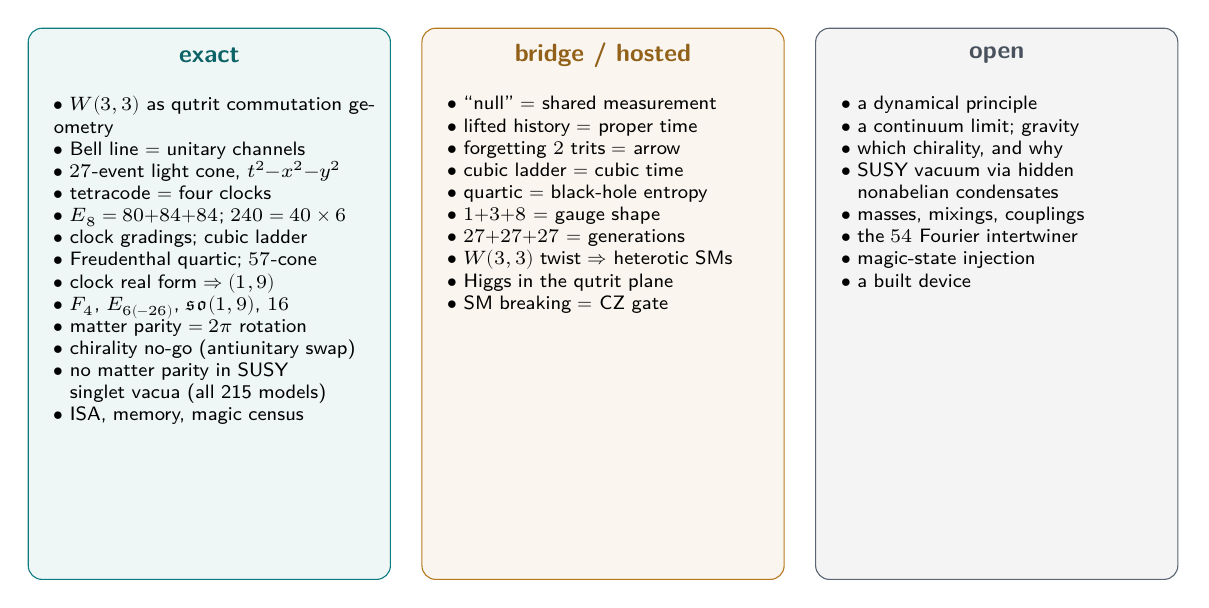
\begin{tikzpicture}[
   col/.style={rounded corners=5pt,draw=#1,fill=#1!7,minimum width=46mm,minimum height=70mm,anchor=north},
   hd/.style={font=\sffamily\small\bfseries,text=#1!80!black},
   it/.style={font=\sffamily\scriptsize,align=left,text width=42mm,anchor=north west}]
  \node[col=teal] at (0,0) {}; \node[hd=teal] at (0,-0.35) {exact};
  \node[it] at (-2.1,-0.75) {$\bullet$ $\W$ as qutrit commutation geometry\\
     $\bullet$ Bell line $=$ unitary channels\\
     $\bullet$ $27$-event light cone, $t^2{-}x^2{-}y^2$\\
     $\bullet$ tetracode $=$ four clocks\\
     $\bullet$ $E_8=80{+}84{+}84$; $240=40\times6$\\
     $\bullet$ clock gradings; cubic ladder\\
     $\bullet$ Freudenthal quartic; $57$-cone\\
     $\bullet$ clock real form $\Rightarrow(1,9)$\\
     $\bullet$ $F_4$, $E_{6(-26)}$, $\so(1,9)$, $16$\\
     $\bullet$ matter parity $=2\pi$ rotation\\
     $\bullet$ chirality no-go (antiunitary swap)\\
     $\bullet$ no matter parity in SUSY\\ \phantom{$\bullet$} singlet vacua (all 215 models)\\
     $\bullet$ ISA, memory, magic census};
  \node[col=gold] at (5.0,0) {}; \node[hd=gold] at (5.0,-0.35) {bridge / hosted};
  \node[it] at (2.9,-0.75) {$\bullet$ ``null'' $=$ shared measurement\\
     $\bullet$ lifted history $=$ proper time\\
     $\bullet$ forgetting $2$ trits $=$ arrow\\
     $\bullet$ cubic ladder $=$ cubic time\\
     $\bullet$ quartic $=$ black-hole entropy\\
     $\bullet$ $1{+}3{+}8$ $=$ gauge shape\\
     $\bullet$ $27{+}27{+}27$ $=$ generations\\
     $\bullet$ $\W$ twist $\Rightarrow$ heterotic SMs\\
     $\bullet$ Higgs in the qutrit plane\\
     $\bullet$ SM breaking $=$ CZ gate};
  \node[col=slate] at (10.0,0) {}; \node[hd=slate] at (10.0,-0.35) {open};
  \node[it] at (7.9,-0.75) {$\bullet$ a dynamical principle\\
     $\bullet$ a continuum limit; gravity\\
     $\bullet$ which chirality, and why\\
     $\bullet$ SUSY vacuum via hidden\\ \phantom{$\bullet$} nonabelian condensates\\
     $\bullet$ masses, mixings, couplings\\
     $\bullet$ the $54$ Fourier intertwiner\\
     $\bullet$ magic-state injection\\
     $\bullet$ a built device};
\end{tikzpicture}
\caption{The state of the programme, in three columns.}
\label{fig:state}
\end{figure}

\subsection{Seven open problems, stated sharply}

\begin{enumerate}[label=\textbf{\arabic*.},leftmargin=1.6em,itemsep=5pt]
\item \textbf{A realistic vacuum.} In singlet directions this is now settled negatively
      (Theorem~9.6): the FI term forces a $B-L=\pm1$ condensate in every model. What remains is
      the hidden nonabelian sector: is there a $D$-flat direction built from hidden $SO(10)$ or
      $SU(2)$ condensates whose parity is compensated by a hidden centre element --- or must the
      programme move to other orbifold groups ($\Z_{12}$, $\Z_2\times\Z_4$, \dots) of the same
      twist? Both are finite computations on the frozen ledger.
\item \textbf{A dynamical principle.} Every result in this paper is kinematics. What
      action, Hamiltonian or spectral principle on $\W$ has the structures found here as its
      symmetries, and what does it predict? In particular: does such a principle select the
      clock real form $E_{8(-24)}$ over the split form --- does the geometry
      \emph{choose} one time?
\item \textbf{A continuum limit.} The finite light cones (in $2+1$, $3+1$, $1+9$ and the
      quartic $57$) are exact algebraic objects. Is there a limit, a tower over $W(3,q)$ or a
      lattice construction, in which one of them becomes a smooth Lorentzian manifold with
      dynamical curvature?
\item \textbf{Chirality from outside.} Corollary~9.7 shows that reversing time's orientation,
      acting antiunitarily and exchanging chirality are one coset, so fixing an arrow makes
      chirality conserved but does not choose it. What physical datum correlates the two ---
      which chirality goes with which direction of time --- and can it come from a vacuum?
\item \textbf{The $54$ intertwiner.} The diagonal clock/phase weld projects onto $54$
      Fourier directions, while the clock grading supplies a canonical $\mathbf{27}\otimes
      \mathbf2$ at degree one. Is there an explicit equivariant isomorphism?
\item \textbf{Numbers.} The up-type Yukawa couplings of the $\Z_6$-I class have a $2+1$
      block structure qualitatively like the observed quark mixing. Can any mass ratio or
      mixing angle be computed, with an error, from a vacuum of the class?
\item \textbf{The machine.} Specify a magic-state injection circuit for the $36$ Witting
      rays with a decoder and a threshold, and build the two-qutrit photonic core.
\end{enumerate}

\subsection{Corrections we kept on the page}

A research record is trustworthy only if it keeps its errors. These were believed,
written down, and then shown false; each correction made the structure \emph{more}
natural, not less.

\begin{center}
\small
\renewcommand{\arraystretch}{1.22}
\begin{tabularx}{\textwidth}{@{}Xp{6.2cm}@{}}
\toprule
\textbf{Was believed} & \textbf{Is true} \\
\midrule
there is a natural bijection $240$ edges $\leftrightarrow$ $240$ roots & no equivariant bijection; a $6{:}1$ fibration of roots over \emph{points} (\S5.4)\\
the Freudenthal $56$ is the clock's $54$ plus $2$ & the $56$ contains only one $27$ of the $54$ (\S6.1)\\
the Albert algebra has ``$27$ minimal idempotents'' as frames & the frames are the $45$ triads (\S6.4)\\
three time bins hold a past and a future qutrit & $\C^3$ cannot hold two qutrits; use time $\otimes$ frequency (\S3.4)\\
the $9$ fixed modes of the spectral clock are the qutrit's $9$ histories & same count, different module (\S4.4)\\
the independence number of $\W$ is $10$ (an ovoid) & it is $7$; $\W$ has no ovoid (\S10.3)\\
at most $34$ of $40$ contexts are classically satisfiable & exactly $36$ (\S10.3)\\
the $\Z_6$-I class is excluded unconditionally & excluded only if matter parity is broken (\S9.3)\\
every $D$-flat support contains a matter-odd singlet (from $60$ samples) & exhaustively true, and the odd singlet always has $B-L=\pm1$ (\S9.4)\\
the three families come from $\W$ & in the orbifolds they come from the three tori (\S9.1)\\
\bottomrule
\end{tabularx}
\end{center}

\begin{keyidea}
The forty points do not yet give a theory of everything. They give something rarer: a
single finite object in which quantum measurement, a light cone, clocks, $E_8$, the
octonionic Albert algebra, ten-dimensional Lorentz symmetry, a chiral spinor, matter parity
and a quantum computer are exact aspects of one structure --- with every claim checkable,
and the remaining distance to physics mapped rather than hidden.
\end{keyidea}

\appendix
\section{The ledger: every claim, its status, its witness}
\label{app:ledger}

Every script named below lives in \texttt{analysis/} of the repository
\texttt{wilcompute/W33-Theory} and writes its certificate to \texttt{data/}; most have a
regression test in \texttt{tests/}. Commit hashes marked ``Holotrade'' refer to the second
research track and are recorded row by row in the ledger of the $\W$ paper.

{\small
\renewcommand{\arraystretch}{1.2}
\begin{longtable}{@{}>{\raggedright\arraybackslash}p{5.9cm}l>{\raggedright\arraybackslash}p{4.9cm}@{}}
\toprule
\textbf{Claim} & \textbf{Badge} & \textbf{Witness}\\
\midrule
\endfirsthead
\toprule
\textbf{Claim} & \textbf{Badge} & \textbf{Witness}\\
\midrule
\endhead
\bottomrule
\endfoot
\multicolumn{3}{@{}l}{\textit{The object and one qutrit (\S\S2--3)}}\\
$\W$: $40$ points, $40$ lines, $\SRG(40,12,2,4)$, spectrum $12,2^{24},(-4)^{15}$ & \tierT & Props.\ 2.1--2.2 (proofs in text)\\
two-sided Weyl maps span $\sll_9$; commutation geometry is $\W$ & \tierT\,\tierC & \cert{w33\_20260924\_temporal\_su9\_e8\_compiler.py}\\
Bell line $=$ unitary-channel diagonal; swap is anti-symplectic & \tierT\,\tierC & \cert{w33\_20260924\_liouville\_swap\_cp\_outer\_bridge.py}\\
transpose induces the outer class (up to labelling gauge) & \tierC & \cert{w33\_20260924\_intrinsic\_transpose\_outer.py}\\
memory witness: Bell fidelity $1-8p/9$, threshold $p=3/4$ & \tierC & \cert{w33\_20260924\_temporal\_quantum\_memory\_witness.py}\\
modular flow of a qutrit state has $A_2$ frequency pattern & \tierC & \cert{w33\_20260924\_modular\_a2\_event\_clock.py}\\
point/line firewall ($27/108/36$ coincidences, non-isomorphic) & \tierC & \cert{w33\_20260924\_history\_pointline\_cospectral\_firewall.py}\\
\multicolumn{3}{@{}l}{\textit{Time (\S4)}}\\
$40=1+12+27$; big cell of $Q(4,3)$ & \tierC & \cert{w33\_20260924\_history\_bigcell\_q43\_compactification.py}\\
finite light cone $t^2-x^2-y^2$; $1+8+6+12$ & \tierT\,\tierC & same\\
$\mathrm{Sym}_2(\F_3)=\F_3^4/\langle1111\rangle$; $D_0+D_\infty+D_++D_-=3I$ & \tierT\,\tierC & \cert{w33\_20260924\_positive\_null\_counter\_cover.py}\\
null graph spectra; $U^3=I$ at $t^\star=2\pi/9$ & \tierC & \cert{w33\_20260924\_null\_history\_spectral\_clock.py}\\
fixed $9$ is not the qutrit module & \tierX & \cert{w33\_20260924\_spectral\_clock\_fixed9\_group\_probe.py}\\
$36$ triangles; unique orientation cycle; $82=1+81$, $81=35+46$ & \tierC & \cert{w33\_20260924\_history\_invariant\_cycle\_orientation.py}\\
filled temporal $H_1$ injects into $H_1(\W)$ & \tierC & \cert{w33\_20260924\_history\_to\_global\_h1\_intertwiner.py}\\
universal cover: $8$-regular tree, $\pi_1=F_{82}$ & \tierT\,\tierC & \cert{w33\_20260924\_temporal\_universal\_cover.py}\\
Weil phase census $1^{13}i^4(-1)^6(-i)^4$; $(FG)^3=iF^2$ & \tierC & \cert{w33\_20260924\_temporal\_maslov\_mu12.py}\\
common $S_4$ of null directions, Hesse clocks, $A_2$ factors & \tierC & \cert{w33\_20260924\_null\_hesse\_4a2\_s4\_intertwiner.py}\\
tetracode $=$ clock evaluation code & \tierC & \cert{w33\_pass10946\_clock\_code\_cone\_objectwise.py}\\
negacyclic hyperbolic pair, $N^4=-I$ (other track) & \tierC & \cert{w33\_pass10948\_clock\_tetracode\_negacyclic\_hyperbolic\_bridge.py}\\
Page--Wootters diagonal weld; $24$ vs $248$ & \tierC & \cert{w33\_20260924\_page\_wootters\_diagonal\_weld.py}\\
Hermitian $3+1$: $21+30+30$; null directions $=$ spread & \tierC & \cert{w33\_20260924\_hermitian\_3p1\_spread\_bridge.py}\\
no compatible complex structure $J$ & \tierX & same\\
forgetting two trits gives the depolarising channel & \tierT & Thm.\ 4.7 (proof in text); \cert{bt823\_the\_closure.py}\\
\multicolumn{3}{@{}l}{\textit{$E_8$ (\S5)}}\\
$E_8=\sll_9+\Lambda^3+\Lambda^6$ as packet operations & \tierC & \cert{w33\_20260924\_temporal\_a8\_e8\_process\_bracket.py}\\
Hesse $4A_2$; $240=72+24+144$ & \tierT\,\tierC & \cert{w33\_20260924\_temporal\_hesse\_4a2\_a8\_bridge.py}\\
no equivariant edge--root bijection & \tierC & \cert{w33\_pass1020\_e8\_transitive\_51840.g}\\
$240=40\times6$ fibration onto points & \tierC & \cert{w33\_pass1021\_e8\_fibration\_over\_forty.g}\\
Hesse clock gradings $1{+}56{+}134{+}56{+}1$ and $|3|$ & \tierC & \cert{w33\_20260925\_hesse\_clock\_e8\_gradings.py}\\
$\Z_3$ grading is the mod-$3$ shadow & \tierC & \cert{w33\_20260925\_e8\_parabolic\_cubic\_clock\_lift.py}\\
cubic ladder $54\to81\to83$; $45$ triads $\times12$ & \tierC & \cert{w33\_20260925\_cubic\_clock\_bracket\_ladder.py}\\
\multicolumn{3}{@{}l}{\textit{Freudenthal, real forms, Albert (\S\S6--8)}}\\
$56$ shares one $27$ with the $54$; $54+2=56$ refuted & \tierC\,\tierX & \cert{w33\_pass10949\_freudenthal\_quasiconformal\_clock\_cone.py}\\
Freudenthal normal form of the quartic, no sign repair & \tierC & same\\
$57$-cone, Heisenberg law, GKN inversion & \tierC & same\\
$K(e_\alpha,e_{-\alpha})=-60(-1)^{\hgt\alpha}$; split $=$ height twist & \tierC & same\\
tick lines: $E_{8(-24)}$, Klein four-group, $80+3\times56$ & \tierC & same\\
Euclidean Albert algebra, Peirce $1+16+10$, $(1,9)$ vs $(5,5)$ & \tierC & same\\
$\mathrm{Der}=F_{4(-52)}$, $\mathrm{str}_0=E_{6(-26)}$ & \tierC & \cert{w33\_pass10950\_clock\_albert\_lorentz\_spinor.py}\\
$\so(1,9)$, Majorana--Weyl $16$; $16=(2,4)+\overline{(2,4)}$ & \tierC & same\\
$Q_\psi=6L_c-2$; matter parity $=\exp(2\pi D)$ & \tierC & same\\
clock $g^4=-I$ is the central $2\pi$ spin sign (other track) & \tierC & \cert{w33\_pass10951\_clock\_pin\_spin\_central\_sign\_bridge.py}\\
Albert $16=8_s+8_c$; half-turn $U^2=-I_{16}$; minimal full-clock carrier $16\oplus16$ (other track) & \tierC & \cert{w33\_pass10956\_albert\_spin8\_halfspin\_normalizer.py}, \cert{w33\_pass10959\_albert\_clock\_extension\_obstruction.py}\\
\multicolumn{3}{@{}l}{\textit{Physics (\S9)}}\\
transvection spine: $648$, $1\oplus3\oplus8$, $9\oplus9\oplus9$ & \tierC\,\tierB & \cert{bt886\_standard\_model\_spine.py}\\
Steinberg: every order-$3$ element splits $27+27+27$ & \tierT & Thm.\ 9.2 (proof in text)\\
no Pauli-spanned $E_6$ on qutrit registers & \tierT\,\tierC & Holotrade \cert{1cde1f1}\\
$\W$ $=$ Pauli geometry of $\Z_3$-twisted $V_{E_8}$ & \tierC & Holotrade \cert{68df33f}\\
order-$3$ orbifold completes no SM family & \tierT\,\tierC & Holotrade \cert{ed1eaca}, \cert{a6e1c69}, \cert{a779053}\\
$\Z_6$: $42$ of $79$ SMs from the $\W$ vacuum & \tierC & Holotrade \cert{5b3f3ad}\\
CZ-type breaking $45/45$; $SU(3)\times SU(2)$ cut $25/25$ & \tierC & Holotrade \cert{d772153}, \cert{94df376}\\
Higgs alone in the qutrit plane; DTS $55/87$ & \tierC & Holotrade \cert{3caf15e}, \cert{a6f1cae}\\
$F$/$D$ conflict; Gordan alternative $215/215$ & \tierC & Holotrade \cert{babfd48}\\
matter parity in all $87$; class closure conditional & \tierC & ledger commit \cert{78ec0a0fc}\\
every sampled $D$-flat support has a matter-odd singlet & \tierC\,\tierO & ledger commit \cert{a3dbdf2d7}\\
chirality no-go & \tierT\,\tierC & \cert{w33\_pass346\_the\_chirality\_no\_go.py}\\
chirality swap is exactly the antiunitary (determinant-odd) coset & \tierC\,\tierB & Holotrade \cert{e92a047}; \cert{w33\_pass10952\_clock\_complete\_positivity\_firewall.py}, \cert{w33\_pass10955\_d4\_halfspin\_clock\_bridge.py}\\
no matter-even SUSY singlet vacuum: $0/88$ over full $B-L$, $0/1024$ $\Z_2$ parities; forced $B-L=\pm1$ condensate & \tierC & \cert{w33\_pass10960\_matter\_even\_dflat\_closure.py}\\
hidden sector: $32$ exact (all directions), $55$ over invariant generators, $1$ by $62{,}309$ rays; anomaly-free models have no parity & \tierC & \cert{w33\_pass10962\_hidden\_sector\_dflat\_tiers.py}, \cert{w33\_pass10962\_tierc\_rays.py}\\
time reversal $=$ antiunitary $=$ chirality swap (one coset) & \tierT & Corollary~9.7 (proof in text)\\
FI acts through $f=4Q_\psi-\tfrac45Q_\chi$; singlet values $\{-8,0,8\}$; forced field $=\nu^c$ of $\mathbf{16}_{-3}\subset\mathbf{78}$ & \tierC\,\tierB & \cert{w33\_pass10964\_e6\_shaped\_fi\_mechanism.py}\\
Baryon triality impossible in $215/215$: $Q(u^c)+Q(e^c)=2Q(q)$ ($SU(5)$) & \tierC & \cert{w33\_pass10965\_baryon\_triality\_impossible.py}\\
Most general matter parity (torus $\times$ space group) survives FI in $0/215$; forced $Q(n)=-Q(u^cd^cd^c)$ in $290/302$; quartic RPV regenerated $23/23$ & \tierC & \cert{w33\_pass10967\_fi\_vacuum\_regenerates\_rpv.py}\\
(Withdrawn by P10974) Plane-rotation $R$-parity under the old per-plane rule: $3/128$; $\Z_6$II$_{23}$ $38$ vacua, exotics massless & \tierC & \cert{w33\_pass10968\_r\_symmetry\_parity\_and\_massless\_exotics.py}\\
$68$-direction vacuum: one parity element, exotics full rank by order $5$, Higgs rank $6$ & \tierC & \cert{w33\_pass10968\_leaf1\_vacuum\_certificate.json}\\
$23$-direction vacuum: exotics full rank, Higgs rank $5/6$ at all orders, $W|_S\neq0$ & \tierC\,\tierO & \cert{w33\_pass10968\_approxR\_vacuum\_certificate.json}\\
$\Z_{12}$-I: $289$ SMs, $14$ parity vacua, exotics massive in none; $\Z_2\times\Z_6$-I: $29$ SMs, $0$ survive & \tierC & \cert{w33\_pass10968\_z12\_left\_chiral\_ledger.json.gz}\\
Harmless RPV needs $\tilde m\gtrsim6\times10^{14}$\,GeV; $\lambda<0$ above $3.2\times10^{10}$\,GeV, so $m_t\le171.0$\,GeV ($5.4\sigma$ low) & \tierC & \cert{w33\_pass10969\_rpv\_heavy\_superpartners\_vs\_higgs\_quartic.py}\\
Established $R$-rules (prime planes $+$ $\gamma$-corrected G2 plane): $\Z_6$II$_{23}$ closes, $\Z_6$-II $0/128$; $\Z_3\times\Z_6$ $0/5$ & \tierC & \cert{w33\_pass10974\_valid\_r\_rules\_close\_the\_rotation\_door.py}\\
\multicolumn{3}{@{}l}{\textit{Machine (\S10)}}\\
$\mathrm{ASp}(4,3)$, $4\,199\,040$; four opcodes; length $19$ & \tierC & blueprint, Passes 2778/2789/2882\\
$4$ stabiliser $+$ $36$ magic rays; KS budget $36/40$; $\alpha=7$ & \tierC & \cert{bt822\_magic\_census\_matter\_is\_magic.py}, \cert{bt818\_ovoid\_nogo\_theta\_gap.py}\\
Steinberg memory $[[240,81,3]]_3$ & \tierC & \cert{bt861\_code\_register\_is\_steinberg.py}\\
Golay lane: $552$ locations, threshold $5.32\times10^{-4}$ & \tierC & \cert{w33\_pass10947\_five\_front\_execution.py}\\
cube-chart atlas; $\le8$ moves per digit & \tierC & \cert{bt777\_hypercube\_chart\_web.py}, \cert{bt827\_holonet\_fractal\_architecture.py}\\
single-photon \textsc{sum} gate, $0.92\pm0.01$ & measured & \cite{Imany2019}\\
\end{longtable}
}

\section{Glossary}
\label{app:glossary}

\newcommand{\gl}[2]{\item[\textsf{\textbf{#1}}] #2}
\begin{description}[leftmargin=0pt,labelsep=0.6em,itemsep=3pt,font=\normalfont]
\gl{$A_2$}{The root system of $SU(3)$: six vectors forming a regular hexagon.}
\gl{Albert algebra}{The $27$-dimensional algebra $H_3(\mathbb O)$ of $3\times3$ Hermitian
  octonionic matrices; the only exceptional Euclidean Jordan algebra.}
\gl{Bell line}{The line of $\W$ formed by the unitary channels $A\mapsto P_uAP_u^\dagger$;
  the ``now'' of Section~4.}
\gl{Bridge}{A true mathematical statement together with a proposed physical reading.}
\gl{Cartan involution}{An involution of a real Lie algebra splitting it into rotations
  ($\mathfrak k$) and boosts ($\mathfrak p$); it fixes the real form.}
\gl{Clifford group}{Quantum operations mapping Pauli operators to Pauli operators; for two
  qutrits it acts on labels as $\Sp(4,3)$.}
\gl{Context}{A maximal set of simultaneously measurable Pauli operators; a line of $\W$.}
\gl{Contextuality}{The impossibility of assigning pre-existing outcomes to all measurements
  consistently across contexts; a resource for quantum computation.}
\gl{CSS code}{A quantum error-correcting code built from two classical codes; $[[n,k,d]]_q$
  means $n$ physical qudits, $k$ logical, distance $d$.}
\gl{$E_8$}{The largest exceptional simple Lie algebra: dimension $248$, $240$ roots.}
\gl{$\F_3$}{The field $\{0,1,2\}$ with arithmetic modulo $3$.}
\gl{Freudenthal triple system}{A $56$-dimensional space with a symplectic form and an
  $E_7$-invariant quartic; the charge space of certain supergravity black holes.}
\gl{Generalized quadrangle}{A point--line geometry with no triangles in which a point off a
  line is collinear with exactly one of its points.}
\gl{Grading}{A splitting of an algebra into pieces labelled by integers (or integers mod
  $n$) that add under the bracket.}
\gl{Hesse clock}{One of the four parallel classes of lines of $AG(2,3)$, read as three ticks.}
\gl{Heisenberg algebra}{The algebra of positions, momenta and a central element; here
  $56+1=57$ dimensions.}
\gl{Heterotic string}{A closed string theory with gauge group $E_8\times E_8$ (or
  $SO(32)$); on orbifolds it yields Standard-Model-like theories.}
\gl{Lagrangian}{A maximal subspace on which the symplectic form vanishes; a line of $\W$.}
\gl{Magic state}{A state that is not a stabiliser state; injecting it makes Clifford
  circuits universal.}
\gl{Majorana--Weyl spinor}{A real, chiral spinor; in ten dimensions it has $16$ components.}
\gl{Matter parity}{A $\Z_2$ symmetry, $-1$ on matter fermions and $+1$ on Higgs fields,
  that forbids fast proton decay in supersymmetric theories.}
\gl{Octonions $\mathbb O$}{The eight-dimensional, non-associative normed division algebra.}
\gl{Orbifold}{A space divided by a finite group; used to curl up extra dimensions.}
\gl{Pauli operator}{For a qutrit, $X^aZ^b$; for two qutrits, a tensor product of two.}
\gl{Peirce decomposition}{The splitting of a Jordan algebra by the eigenvalues $1,\tfrac12,0$
  of multiplication by an idempotent.}
\gl{Qutrit}{A quantum system with three perfectly distinguishable states.}
\gl{Real form}{A real Lie algebra whose complexification is a given complex one; $E_8$ has
  three.}
\gl{Root}{An eigen-direction of the maximal commuting part of a Lie algebra.}
\gl{Signature}{For a quadratic form, the numbers of positive and negative directions; for a
  real Lie algebra, $\dim\mathfrak p-\dim\mathfrak k$.}
\gl{Spread}{A set of pairwise disjoint lines covering every point; $\W$ has $36$.}
\gl{Steinberg module}{A distinguished irreducible representation of a finite group of Lie
  type; for $\PSp(4,3)$ it is $81$-dimensional and is $H_1(\W)$.}
\gl{Stabiliser state}{A joint eigenstate of a maximal commuting set of Paulis.}
\gl{Strongly regular graph}{A regular graph in which adjacent pairs have $\lambda$, and
  non-adjacent pairs $\mu$, common neighbours.}
\gl{Symplectic form}{An alternating, nondegenerate bilinear form; here the commutation
  phase of Pauli operators.}
\gl{Tetracode}{The ternary $[4,2,3]$ code; here the evaluation code of the four clocks.}
\gl{Transvection}{The symplectic map $x\mapsto x+\langle x,v\rangle v$.}
\gl{Tripotent}{An element $e$ of a Jordan triple system with $\{e,e,e\}=2e$ (normalisation
  of this paper).}
\gl{Witting polytope}{A regular complex polytope in $\C^4$ with $240$ vertices, the $E_8$
  roots, and $40$ diameters.}
\end{description}

\begin{thebibliography}{99}
\addcontentsline{toc}{section}{References}
\small

\bibitem{Adams1996} J.~F. Adams, \emph{Lectures on Exceptional Lie Groups}, University of
Chicago Press, 1996.

\bibitem{Baez2002} J.~C. Baez, The octonions, \emph{Bull.\ Amer.\ Math.\ Soc.} \textbf{39}
(2002) 145--205.

\bibitem{BaezHuerta} J.~C. Baez and J.~Huerta, Division algebras and supersymmetry I, in
\emph{Superstrings, Geometry, Topology, and $C^*$-algebras}, Proc.\ Symp.\ Pure Math.\
\textbf{81} (2010) 65--80, arXiv:0909.0551.

\bibitem{BDDER} L.~Borsten, D.~Dahanayake, M.~J. Duff, H.~Ebrahim and W.~Rubens, Black
holes, qubits and octonions, \emph{Phys.\ Rep.} \textbf{471} (2009) 113--219,
arXiv:0809.4685.

\bibitem{BvM} A.~E. Brouwer and H.~Van Maldeghem, \emph{Strongly Regular Graphs},
Cambridge University Press, 2022.

\bibitem{ConnesRovelli} A.~Connes and C.~Rovelli, Von Neumann algebra automorphisms and
time--thermodynamics relation in generally covariant quantum theories, \emph{Class.\
Quantum Grav.} \textbf{11} (1994) 2899--2918.

\bibitem{ConwaySloane} J.~H. Conway and N.~J.~A. Sloane, \emph{Sphere Packings, Lattices and
Groups}, 3rd ed., Springer, 1999.

\bibitem{DHVW} L.~Dixon, J.~A. Harvey, C.~Vafa and E.~Witten, Strings on orbifolds,
\emph{Nucl.\ Phys.} \textbf{B261} (1985) 678--686.

\bibitem{DuffFerrara} M.~J. Duff and S.~Ferrara, $E_7$ and the tripartite entanglement of
seven qubits, \emph{Phys.\ Rev.\ D} \textbf{76} (2007) 025018, arXiv:quant-ph/0609227.

\bibitem{FarautKoranyi} J.~Faraut and A.~Kor\'anyi, \emph{Analysis on Symmetric Cones},
Oxford University Press, 1994.

\bibitem{Freudenthal} H.~Freudenthal, Beziehungen der $E_7$ und $E_8$ zur Oktavenebene I,
\emph{Indag.\ Math.} \textbf{16} (1954) 218--230.

\bibitem{Garibaldi} S.~Garibaldi, $E_8$, the most exceptional group, \emph{Bull.\ Amer.\
Math.\ Soc.} \textbf{53} (2016) 643--671.

\bibitem{GHW} K.~S. Gibbons, M.~J. Hoffman and W.~K. Wootters, Discrete phase space based on
finite fields, \emph{Phys.\ Rev.\ A} \textbf{70} (2004) 062101.

\bibitem{GKN} M.~G\"unaydin, K.~Koepsell and H.~Nicolai, Conformal and quasiconformal
realizations of exceptional Lie groups, \emph{Commun.\ Math.\ Phys.} \textbf{221} (2001)
57--76, arXiv:hep-th/0008063.

\bibitem{GST1983} M.~G\"unaydin, G.~Sierra and P.~K. Townsend, Exceptional supergravity
theories and the magic square, \emph{Phys.\ Lett.} \textbf{B133} (1983) 72--76.

\bibitem{Gunaydin1993} M.~G\"unaydin, Generalized conformal and superconformal group actions
and Jordan algebras, \emph{Mod.\ Phys.\ Lett.\ A} \textbf{8} (1993) 1407--1416,
arXiv:hep-th/9301050.

\bibitem{Howard2014} M.~Howard, J.~Wallman, V.~Veitch and J.~Emerson, Contextuality supplies
the `magic' for quantum computation, \emph{Nature} \textbf{510} (2014) 351--355.

\bibitem{Humphreys} J.~E. Humphreys, The Steinberg representation, \emph{Bull.\ Amer.\
Math.\ Soc.} \textbf{16} (1987) 247--263.

\bibitem{Imany2019} P.~Imany, J.~A. Jaramillo-Villegas, M.~S. Alshaykh, J.~M. Lukens,
O.~D. Odele, A.~J. Moore, D.~E. Leaird, M.~Qi and A.~M. Weiner, High-dimensional optical
quantum logic in large operational spaces, \emph{npj Quantum Inf.} \textbf{5} (2019) 59.

\bibitem{KalloshKol} R.~Kallosh and B.~Kol, $E_7$ symmetric area of the black hole horizon,
\emph{Phys.\ Rev.\ D} \textbf{53} (1996) R5344, arXiv:hep-th/9602014.

\bibitem{KRZ2020} H.~Kraft, A.~Regeta and S.~Zimmermann, Small $G$-varieties,
arXiv:2009.05559.

\bibitem{Krutelevich} S.~Krutelevich, Jordan algebras, exceptional groups and Bhargava
composition, \emph{J.\ Algebra} \textbf{314} (2007) 924--977.

\bibitem{KugoTownsend} T.~Kugo and P.~Townsend, Supersymmetry and the division algebras,
\emph{Nucl.\ Phys.} \textbf{B221} (1983) 357--380.

\bibitem{Landauer} R.~Landauer, Irreversibility and heat generation in the computing
process, \emph{IBM J.\ Res.\ Dev.} \textbf{5} (1961) 183--191.

\bibitem{Lebedev2008} O.~Lebedev, H.~P. Nilles, S.~Raby, S.~Ramos-S\'anchez, M.~Ratz,
P.~K.~S. Vaudrevange and A.~Wingerter, The heterotic road to the MSSM with R parity,
\emph{Phys.\ Rev.\ D} \textbf{77} (2008) 046013, arXiv:0708.2691.

\bibitem{LloydBraunstein} S.~Lloyd and S.~L. Braunstein, Quantum computation over
continuous variables, \emph{Phys.\ Rev.\ Lett.} \textbf{82} (1999) 1784--1787.

\bibitem{MDW2022} C.~A. Manogue, T.~Dray and R.~A. Wilson, Octions: an $E_8$ description of
the Standard Model, \emph{J.\ Math.\ Phys.} \textbf{63} (2022) 081703, arXiv:2204.05310.

\bibitem{Martin1992} S.~P. Martin, Some simple criteria for gauged R-parity, \emph{Phys.\
Rev.\ D} \textbf{46} (1992) R2769, arXiv:hep-ph/9207218.

\bibitem{Orbifolder} H.~P. Nilles, S.~Ramos-S\'anchez, P.~K.~S. Vaudrevange and
A.~Wingerter, The Orbifolder: a tool to study the low-energy effective theory of heterotic
orbifolds, \emph{Comput.\ Phys.\ Commun.} \textbf{183} (2012) 1363--1380, arXiv:1110.5229.

\bibitem{PageWootters} D.~N. Page and W.~K. Wootters, Evolution without evolution: dynamics
described by stationary observables, \emph{Phys.\ Rev.\ D} \textbf{27} (1983) 2885--2892.

\bibitem{PayneThas} S.~E. Payne and J.~A. Thas, \emph{Finite Generalized Quadrangles}, 2nd
ed., European Mathematical Society, 2009.

\bibitem{Springer} T.~A. Springer, Regular elements of finite reflection groups,
\emph{Invent.\ Math.} \textbf{25} (1974) 159--198.

\bibitem{Tegmark1997} M.~Tegmark, On the dimensionality of spacetime, \emph{Class.\ Quantum
Grav.} \textbf{14} (1997) L69--L75, arXiv:gr-qc/9702052.

\bibitem{WBCV2018} Watanabe, Belfiore, de Carvalho and Vieira Filho, a cyclotomic
construction of $E_8$ from the negacyclic tetracode, \emph{Int.\ J.\ Appl.\ Math.}
\textbf{31}(1) (2018), doi:10.12732/ijam.v31i1.6 (as cited in Pass~10948).

\end{thebibliography}


\end{document}
